\documentclass[DM,lsstdraft,toc]{lsstdoc}

% lsstdoc documentation: https://lsst-texmf.lsst.io/lsstdoc.html


% Package imports go here.


% Local commands go here.

% To add a short-form title:
% \title[Short title]{Title}
\title{Data Management Database Design}

% Optional subtitle
% \setDocSubtitle{A subtitle}

\author{%
	Jacek Becla,
	Daniel Wang,
	Serge Monkewitz,
	K-T Lim,
	John Gates,
	Andy Salnikov,
	Andrew Hanushevsky,
	Douglas Smith,
	Bill Chickering,
	Michael Kelsey,
	and
	Fritz Mueller
}

\setDocRef{LDM-135}

\date{\today}

% Optional: name of the document's curator
% \setDocCurator{The Curator of this Document}

\setDocAbstract{%
This document discusses the LSST database system architecture.
}


% Change history defined here.
% Order: oldest first.
% Fields: VERSION, DATE, DESCRIPTION, OWNER NAME.
% See LPM-51 for version number policy.
\setDocChangeRecord{%
  \addtohist{1.0}{2009-06-15}{Initial version.}{Jacek Becla}
  \addtohist{2.0}{2011-07-12}{Most sections rewritten, added scalability test section}{Jacek Becla}
  \addtohist{2.1}{2011-08-12}{Refreshed future-plans and schedule of testing sections, added section about fault tolerance.}{Jacek Becla, Daniel Wang}
  \addtohist{3.0}{2013-08-02}{Synchronized with latest changes to the requirements (LSE-163). Rewrote most of the “Implementation” chapter. Documented new tests, refreshed all other chapters.}{Jacek Becla, Daniel Wang, Serge Monkewitz, Kian-Tat Lim, Douglas Smith, Bill Chickering}
  \addtohist{3.1}{2013-10-10}{Refreshed numbers based on latest LDM-141. Updated shared scans (implementation) and 300-node test sections, added section about shared scans demonstration}{Jacek Becla, Daniel Wang}
  \addtohist{3.2}{2013-10-10}{TCT approved}{R Allsman}
  \addtohist{draft}{2016-07-18}{Update with async query, shared scan, secondary index, xrootd, metadata service information.}{John Gates, Andy Salnikov, Andrew Hanushevsky, Michael Kelsey, Fritz Mueller}
}

\begin{document}
\makeatletter
\renewcommand{\l@section}{\@dottedtocline{1}{1.5em}{2.6em}}
\renewcommand{\l@subsection}{\@dottedtocline{2}{4.0em}{3.6em}}
\renewcommand{\l@subsubsection}{\@dottedtocline{3}{7.4em}{4.5em}}
\makeatother

% Create the title page.
% Table of contents is added automatically with the "toc" class option.
\maketitle

\section{Executive Summary}\label{executive-summary}

The LSST baseline database architecture for its massive user query
access system is an MPP (massively parallel processing) relational
database composed of a single-node non-parallel DBMS, a distributed
communications layer, and a master controller, all running on a
shared-nothing cluster of commodity servers with locally attached
spinning disk drives, capable of incremental scaling and recovering from
hardware failures without disrupting running queries. All large catalogs
are spatially partitioned horizontally into materialized \emph{chunks},
and the remaining catalogs are replicated on each server; the chunks are
distributed across all nodes. The Object catalog is further partitioned
into \emph{sub-chunks} with overlaps, materialized on-the-fly when
needed. Chunking is handled automatically without exposure to users.
Selected tables are also partitioned vertically to maximize performance
of most common analysis. The system uses a few critical indexes to speed
up spatial searches, time series analysis, and simple but interactive
queries. Shared scans are used to answer all but the interactive
queries. Such an architecture is primarily driven by the variety and
complexity of anticipated queries, ranging from single object lookups to
complex \(O(n^2)\) full-sky correlations over billions of elements.

The LSST baseline database architecture for its real time Alert
Production relies on horizontal time-based partitioning. To guarantee
reproducibility, no-overwrite-update techniques combined with
maintaining validity time for appropriate rows are employed. Two
database replicas are maintained to isolate live production catalogs
from user queries; the replicas are synchronized in real time using
native database replication.

Given the current state of the RDBMS and Map/Reduce market, an
RDBMS-based solution is a much better fit, primarily due to features
such as indexes, schema and speed. No off-the-shelf, reasonably priced
solution meets our requirements (today), even though production systems
at a scale comparable to LSST have been demonstrated already by
industrial users such as eBay using a prohibitively expensive,
commercial RDBMS.

The baseline design involves many choices such as component technology,
partition size, index usage, normalization level, compression
trade-offs, applicability of technologies such as solid state disks,
ingest techniques and others. We ran many tests to determine the design
configuration, determine limits and uncover potential bottlenecks. In
particular, we chose \emph{MySQL} as our baseline open source,
single-node DBMS and \href{http://xrootd.org}{XRootD} as an open source,
elastic, distributed, fault-tolerant messaging system.

We developed a prototype of the baseline architecture, called
\emph{Qserv}. To mitigate major risks, such as insufficient scalability
or potential future problems with the underlying RDBMS, Qserv pays close
attention to minimizing exposure to vendor-specific features and
add-ons. Many key features including the scalable dispatch system and
2-level partitioner have been implemented at the prototype level and
integrated with the two underlying production-quality components: MySQL
and \href{http://xrootd.org}{XRootD}. Scalability and performance have
been successfully demonstrated on a variety of clusters ranging from
20-node-100TB cluster to 300-node-30TB cluster, tables as large as 50
billion rows and concurrency exceeding 100,000 in-flight chunk-queries.
Required data rates for all types of queries (interactive, full sky
scans, joins, correlations) have been achieved. Basic fault tolerance
recovery mechanisms and basic version of shared scans were demonstrated.
Future work includes adding support for user tables, demonstrating
cross-matching, various non-critical optimizations, and most
importantly, making the prototype more user-friendly and turning it into
a production-ready system.

If an equivalent open-source, community supported, off-the-shelf
database system were to become available, it could present significant
support cost advantages over a production-ready Qserv. The largest
barrier preventing us from using an off-the-shelf system is spherical
geometry and spherical partitioning support.

To increase the chances such a system will become reality in the next
few years, in 2008 we initiated the SciDB array-based scientific
database project. Due to lack of many traditional RDBMS-features in
SciDB and still nascent fault tolerance, we believe it is easier to
build the LSST database system using
MySQL+\href{http://xrootd.org}{XRootD} than it would be to build it
based on SciDB. In addition we closely collaborate with the MonetDB open
source columnar database team -- a successful demonstration of Qserv
based on MonetDB instead of MySQL was done in 2012. Further, to stay
current with the state-of-the-art in peta-scale data management and
analysis, we continue a dialog with all relevant solution providers,
both DBMS and Map/Reduce, as well as with data-intensive users, both
industrial and scientific, through the \href{http://xldb.org}{XLDB}
conference series we lead, and beyond.

\section{Introduction}\label{introduction}

This document discusses the LSST database system architecture. Chapter~\ref{baseline-architecture} discusses the baseline
architecture. Chapter~\ref{requirements} explains the LSST database-related
requirements. Chapter~\ref{potential-solutions} covers in-depth analysis
of existing off-the-shelf potential solutions (Map/Reduce and RDBMS).
Chapter~\ref{design-trade-offs} discusses design trade-offs
and decision process, including small scale tests we run.
Chapter~\ref{risk-analysis} covers risk analysis.
Chapter~\ref{implementation} discusses the
prototype design (Qserv), including design, current status of the
software and future plans.
Chapters~\ref{large-scale-testing} and \ref{other-demonstrations}
describe large scale Qserv
tests and demonstrations.

\section{Baseline Architecture}\label{baseline-architecture}

This chapter describes the most important aspects of the LSST baseline
database architecture. The choice of the architecture is driven by the
project requirements (see reqs) as well as cost, availability and
maturity of the off-the-shelf solutions currently available on the
market (see Chapter~\ref{potential-solutions}), and design trade-offs (see
Chapter~\ref{design-trade-offs}). The architecture is periodically revisited: we
continuously monitor all relevant technologies, and accordingly
fine-tune the baseline architecture.

In summary, the LSST baseline architecture for Alert Production is an
off-the-shelf RDBMS system which uses replication for fault tolerance
and which takes advantage of horizontal (time-based) partitioning. The
baseline architecture for user access to Data Releases is an MPP
(multi-processor, parallel) relational database running on a
shared-nothing cluster of commodity servers with locally attached
spinning disk drives; capable of (a) incremental scaling and (b)
recovering from hardware failures without disrupting running queries.
All large catalogs are spatially partitioned into materialized
\emph{chunks}, and the remaining catalogs are replicated on each server;
the chunks are distributed across all nodes. The Object catalog is
further partitioned into \emph{sub-chunks} with overlaps,\footnote{A
  chunk's overlap is implicitly contained within the overlaps of its
  edge sub-chunks.} materialized on-the-fly when needed. Shared scans
are used to answer all but low-volume user queries. Details follow
below.

\subsection{Alert Production and Up-to-date
Catalog}\label{alert-production-and-up-to-date-catalog}

Alert Production involves detection and measurement of
difference-image-analysis sources (DiaSources). New DiaSources are
spatially matched against the most recent versions of existing
DiaObjects, which contain summary properties for variable and transient
objects (and false positives). Unmatched DiaSources are used to create
new DiaObjects. If a DiaObject has an associated DiaSource that is no
more than a month old, then a forced measurement (DiaForcedSource) is
taken at the position of that object, whether a corresponding DiaSource
was detected in the exposure or not.

The output of Alert Production consists mainly of three large catalogs
-- DiaObject, DiaSource, and DiaForcedSource - as well as several
smaller tables that capture information about e.g. exposures, visits and
provenance.

These catalogs will be modified live every night. After Data Release
Production has been run based on the first six months of data and each
year's data thereafter, the live Level 1 catalogs will be archived to
tape and replaced by the catalogs produced by DRP. The archived catalogs
will remain available for bulk download, but not for queries.

Note that existing DiaObjects are never overwritten. Instead, new
versions of the AP-produced and DRP-produced DiaObjects are inserted,
allowing users to retrieve (for example) the properties of DiaObjects as
known to the pipeline when alerts were issued against them. To enable
historical queries, each DiaObject row is tagged with a validity start
and end time. The start time of a new DiaObject version is set to the
observation time of the DiaSource or DiaForcedSource that led to its
creation, and the end time is set to infinity. If a prior version
exists, then its validity end time is updated (in place) to equal the
start time of the new version. As a result, the most recent versions of
DiaObjects can always be retrieved with:

\begin{lstlisting}[language=SQL]
SELECT * FROM DiaObject WHERE validityEnd = infinity
\end{lstlisting}

Versions as of some time \emph{t} are retrievable via:

\begin{lstlisting}[language=SQL]
SELECT * FROM DiaObject WHERE validityStart <= t AND t < validityEnd
\end{lstlisting}

Note that a DiaSource can also be reassociated to a solar-system object
during day time processing. This will result in a new DiaObject version
unless the DiaObject no longer has any associated DiaSources. In that
case, the validity end time of the existing version is set to the time
at which the reassociation occurred.

Once a DiaSource is associated with a solar system object, it is never
associated back to a DiaObject. Therefore, rather than also versioning
DiaSources, columns for the IDs of both the associated DiaObject and
solar system object, as well as a reassociation time, are included.
Reassociation will set the solar system object ID and reassociation
time, so that DiaSources for DiaObject 123 at time \emph{t} can be
obtained using:

\begin{lstlisting}[language=SQL]
SELECT *
FROM DiaSource
WHERE diaObjectId = 123
AND midPointTai <= t
AND (ssObjectId is NULL OR ssObjectReassocTime > t)
\end{lstlisting}

DiaForcedSources are never reassociated or updated in any way.

From the database point of view then, the alert production pipeline will
perform the following database operations 189 times (once per LSST CCD)
per visit (every 39 seconds):

\begin{enumerate}
\def\labelenumi{\arabic{enumi}.}
\item
  Issue a point-in-region query against the DiaObject catalog, returning
  the most recent versions of the objects falling inside the CCD.
\item
  Use the IDs of these diaObjects to retrieve all associated diaSources
  and diaForcedSources.
\item
  Insert new diaSources and diaForcedSources.
\item
  Update validity end times of diaObjects that will be superseded.
\item
  Insert new versions of diaObjects.
\end{enumerate}

All spatial joins will be performed on in-memory data by pipeline code,
rather than in the database. While Alert Production does also involve a
spatial join against the Level 2 (DRP-produced) Object catalog, this
does not require any database interaction: Level 2 Objects are never
modified, so the Object columns required for spatial matching will be
dumped to compact binary files once per Data Release. These files will
be laid out in a way that allows for very fast region queries, allowing
the database to be bypassed entirely.

The DiaSource and DiaForcedSource tables will be split into two tables,
one for historical data and one containing records inserted during the
current night. The current-night tables will be small and rely on a
transactional engine like InnoDB, allowing for speedy recovery from
failures. The historical-data tables will use the faster
non-transactional MyISAM or Aria storage engine, and will also take
advantage of partitioning. The Data Release catalogs used to seed the
live catalogs will be stored in a single initial partition, sorted
spatially (using the Hierarchical Triangular Mesh trixel IDs for their
positions). This means that the diaSources and diaForcedSources for the
diaObjects in a CCD will be located close together on disk, minimizing
seeks. Every month of new data will be stored in a fresh partition,
again sorted spatially. Such partitions will grow to contain just a few
billion rows over the course of a month, even for the largest catalog.
At the end of each night, the contents of the current-night table are
sorted and appended to the partition for the current-month, then
emptied. Each month, the entire current-month partition is sorted
spatially (during the day), and a partition for the next month is
created.

For DiaObject, the same approach is used. However, DiaObject validity
end-time updates can occur in any partition, and are not confined to the
current-night table. We therefore expect to use a transactional storage
engine like InnoDB for all partitions. Because InnoDB clusters tables
using the primary key, we will likely declare it to consist of a leading
HTM ID column, followed by disambiguating columns (diaObjectId,
validityStart). The validity end time column will not be part of any
index.

No user queries will be allowed on the live production catalogs. We
expect to maintain a separate replica just for user queries,
synchronized in real time using one-way master-slave native database
replication. The catalogs for user queries will be structured
identically to the live catalogs, and views will be used to hide the
splits (using a ``\texttt{UNION\ ALL}'').

For additional safety, we might choose to replicate the small
current-night tables, all DiaObject partitions, and the remaining
(small) changing tables to another hot stand-by replica. In case of
disastrous master failure that cannot be fixed rapidly, the slave
serving user queries will be used as a temporary replacement, and user
queries will be disallowed until the problem is resolved.

Based on the science requirements, only short-running, relatively simple
user queries will be needed on the Level 1 catalogs. The most complex
queries, such as large-area near neighbor queries, will not be needed.
Instead, user queries will consist mainly of small-area cone searches,
light curve lookups, and historical versions of the same. Since the
catalogs are sorted spatially, we expect to be able to quickly answer
spatial queries using indexed HTM ID columns and the scisql UDFs, an
approach that has worked well in data-challenges to date. Furthermore,
note that the positions of diaSources/diaForcedSources associated with
the same diaObject will be very close together, so that sorting to
obtain good spatial locality also ends up placing sources belonging to
the same light curve close together. In other words, the data
organization used to provide fast pipeline query response is also
advantageous for user queries.

\subsection{Data Release Production}\label{data-release-production}

Data Release Production will involve the generation of significantly
larger catalogs than Alert Production. However, these are produced over
the course of several months, pipelines will not write directly to the
database, and there are no pipeline queries with very low-latency
execution time requirements to be satisfied. While we do expect several
pipeline-related full table scans over the course of a Data Release
Production, we will need to satisfy many user queries involving such
scans on a daily basis. User query access is therefore the primary
driver of our scalable database architecture, which is described in
detail below. For a description of the data loading process, please see
qserve-data-loading.

\subsection{User Query Access}\label{user-query-access}

The user query access is the primary driver of the scalable database
architecture. Such architecture is described below.

\subsubsection{Distributed and parallel}\label{distributed-and-parallel}

The database architecture for user query access relies on a model of
distributing computation among autonomous worker nodes. Autonomous
workers have no direct knowledge of each other and can complete their
assigned work without data or management from their peers. This implies
that data must be partitioned, and the system must be capable of
dividing a single user query into sub-queries, and executing these
sub-queries in parallel -- running a high-volume query without
parallelizing it would take unacceptably long time, even if run on very
fast CPU. The parallelism and data distribution should be handled
automatically by the system and hidden from users.

\subsubsection{Shared-nothing}\label{shared-nothing}

Such architecture provides good foundation for incremental scaling and
fault recovery: because nodes have no direct knowledge of each other and
can complete their assigned work without data or management from their
peers, it is possible to add node to, or remove node from such system
with no (or with minimal) disruption. However, to achieve fault
tolerance and provide recover mechanisms, appropriate smarts have to be
build into the node management software.

\begin{figure}[H]
\centering
\includegraphics{_static/shared_nothing_arch.jpg}
\caption{Shared-nothing database architecture.}
\end{figure}

\subsubsection{Indexing}\label{indexing}

Disk I/O bandwidth is expected to be the greatest bottleneck. Data can
be accessed either through index, which typically translates to a random
access, or a scan, which translates to a sequential read (unless
multiple competing scans are involved).

Indexes dramatically speed up locating individual rows, and avoid
expensive full table scans. They are essential to answer low volume
queries quickly, and to do efficient table joins. Also, spatial indexes
are essential. However, unlike in traditional, small-scale systems, the
advantages of indexes become questionable when a larger number of rows
is to be selected from a table. In case of LSST, selecting even a 0.01\%
of a table might lead to selecting millions of rows. Since each fetch
through an index might turn into a disk seek, it is often cheaper to
read sequentially from disk than to seek for particular rows via index,
especially when the index itself is out-of-memory. For that reason the
architecture forgoes relying on heavy indexing, only a small number of
carefully selected indexes essential for answering low-volume queries,
enabling table joins, and speeding up spatial searches will be
maintained. For an analytical query system, it makes sense to make as
few assumptions as possible about what will be important to our users,
and to try and provide reasonable performance for as broad a query load
as possible, i.e. focus on scan throughput rather than optimizing
indexes. A further benefit to this approach is that many different
queries are likely to be able to share scan IO, boosting system
throughput, whereas caching index lookup results is likely to provide
far fewer opportunities for sharing as the query count scales (for the
amounts of cache we can afford).

\subsubsection{Shared scanning}\label{shared-scanning}

Now with table-scanning being the norm rather than the exception and
each scan taking a significant amount of time, multiple full-scan
queries would randomize disk access if they each employed their own
full-scanning read from disk. Shared scanning (also called \emph{convoy
scheduling}) shares the I/O from each scan with multiple queries. The
table is read in pieces, and all concerning queries operate on that
piece while it is in memory. In this way, results from many full-scan
queries can be returned in little more than the time for a single
full-scan query. Shared scanning also lowers the cost of data
compression by amortizing the CPU cost among the sharing queries,
tilting the tradeoff of increased CPU cost versus reduced I/O cost
heavily in favor of compression.

Shared scanning will be used for all high-volume and super-high volume
queries. Shared scanning is helpful for unpredictable, ad-hoc analysis,
where it prevents the extra load from increasing the disk /IO cost --
only more CPU is needed. On average we expect to continuously run the
following scans:

\begin{itemize}
\item
  one full table scan of Object table for the latest data release only,
\item
  one synchronized full table scan of Object, Source and ForcedSource
  tables every 12 hours for the latest data release only,
\item
  one synchronized full table scan of Object and Object\_Extra every 8
  hours for the latest and previous data releases.
\end{itemize}

Appropriate Level 3 user tables will be scanned as part of each shared
scan as needed to answer any in-flight user queries.

Shared scans will take advantage of table chunking explained below. In
practice, within a single node a scan will involve fetching sequentially
a chunk of data at a time and executing on this chunk all queries in the
queue. The level of parallelism will depend on the number of available
cores.

Running multiple shared scans allows relatively fast response time for
Object-only queries, and supporting complex, multi-table joins:
synchronized scans are required for two-way joins between different
tables. For a self-joins, a single shared scans will be sufficient,
however each node must have sufficient memory to hold 2 chunks at any
given time (the processed chunk and next chunk). Refer to the sizing
model {[}LDM-141{]}\_ for further details on the cost of shared scans.

Low-volume queries will be executed ad-hoc, interleaved with the shared
scans. Given the number of spinning disks is much larger than the number
of low-volume queries running at any given time, this will have very
limited impact on the sequential disk I/O of the scans, as shown in
{[}LDM-141{]}\_.

\subsubsection{Clustering}\label{clustering}

The data in the Object Catalog will be physically clustered on disk
spatially -- that means that objects collocated in space will be also
collocated on disk. All Source-type catalogs (Source, ForcedSource,
DiaSource, DiaForcedSource) will be clustered based on their
corresponding objectId -- this approach enforces spatial clustering and
collocates sources belonging to the same object, allowing sequential
read for queries that involve times series analysis.

SSObject catalog will be unpartitioned, because there is no obvious
fixed position that we could choose to use for partitioning. The
associated diaSources (which will be intermixed with diaSources
associated with static diaSources) will be partitioned, according their
position. For that reason the SSObject-to-DiaSource join queries will
require index searches on all chunks, unlike DiaObject-to-DiaSource
queries. Since SSObject is small (low millions), this should not be an
issue.

\subsubsection{Partitioning}\label{partitioning}

Data must be partitioned among nodes in a shared-nothing architecture.
While some \emph{sharding} approaches partition data based on a hash of
the primary key, this approach is unusable for LSST data since it
eliminates optimizations based on celestial objects' spatial nature.

\paragraph{Sharded data and sharded
queries}\label{sharded-data-and-sharded-queries}

All catalogs that require spatial partitioning (Object, Source,
ForcedSource, DiaSource, DiaForcedSource) as well as all the auxiliary
tables associated with them, such as ObjectType, or PhotoZ, will be
divided into spatial partitions of roughly the same area by partitioning
then into \emph{declination} zones, and chunking each zone into
\emph{RA} stripes. Further, to be able to perform table joins without
expensive inter-node data transfers, partitioning boundaries for each
partitioned table must be aligned, and chunks of different tables
corresponding to the same area of sky must be co-located on the same
node. To ensure chunks are appropriately sized, the two largest
catalogs, Source and ForcedSource, are expected to be partitioned into
finer-grain chunks. Since objects occur at an approximately-constant
density throughout the celestial sphere, an equal-area partition should
spread a load that is uniformly distributed over the sky.

Smaller catalogs that can be partitioned spatially, such as Alert and
exposure metadata will be partitioned spatially. All remaining catalogs,
such provenance or SDQA tables will be replicated on each node. The size
of these catalogs is expected to be only a few terabytes.

With data in separate physical partitions, user queries are themselves
fragmented into separate physical queries to be executed on partitions.
Each physical query's result can be combined into a single final result.

\paragraph{Two-level partitions}\label{two-level-partitions}

Determining the size and number of data partitions may not be obvious.
Queries are fragmented according to partitions so an increasing number
of partitions increases the number of physical queries to be dispatched,
managed, and aggregated. Thus a greater number of partitions increases
the potential for parallelism but also increases the overhead. For a
data-intensive and bandwidth-limited query, a parallelization width
close to the number of disk spindles should minimize seeks and
maximizing bandwidth and performance.

From a management perspective, more partitions facilitate rebalancing
data among nodes when nodes are added or removed. If the number of
partitions were equal to the number of nodes, then the addition of a new
node would require the data to be re-partitioned. On the other hand, if
there were many more partitions than nodes, then a set of partitions
could be assigned to the new node without re-computing partition
boundaries.

Smaller and more numerous partitions benefit spatial joins. In an
astronomical context, we are interested in objects near other objects,
and thus a full \(O(n^2)\) join is not required--a localized spatial
join is more appropriate. With spatial data split into smaller
partitions, an SQL engine computing the join need not even consider (and
reject) all possible pairs of objects, merely all the pairs within a
region. Thus a task that is \(O(n^2)\) naively becomes \(O(kn)\) where
\(k\) is the number of objects in a partition.

In consideration of these trade-offs, two-level partitioning seems to be
a conceptually simple way to blend the advantages of both extremes.
Queries can be fragmented in terms of coarse partitions (``chunks''),
and spatial near-neighbor joins can be executed over more fine
partitions (``sub-chunks'') within each partition. To avoid the overhead
of the sub-chunks for non-join queries, the system can store chunks and
generate sub-chunks on-demand for spatial join queries. On-the-fly
generation for joins is cost-effective due to the drastic reduction of
pairs, which is true as long as there are many sub-chunks for each
chunk.

\paragraph{Overlap}\label{overlap}

A strict partitioning eliminates nearby pairs where objects from
adjacent partitions are paired. To produce correct results under strict
partitioning, nodes need access to objects from outside partitions,
which means that data exchange is required. To avoid this, each
partition can be stored with a pre-computed amount of overlapping data.
This overlapping data does not strictly belong to the partition but is
within a preset spatial distance from the partition's borders. Using
this data, spatial joins can be computed correctly within the preset
distance without needing data from other partitions that may be on other
nodes.

Overlap is needed only for the Object Catalog, as all spatial
correlations will be run on that catalog only. Guided by the experience
from other projects including SDSS, we expect to preset the overlap to
\textasciitilde{}1 arcmin, which results in duplicating approximately
30\% of the Object Catalog.

\paragraph{Spherical geometry}\label{spherical-geometry}

Support for spherical geometry is not common among databases and
spherical geometry-based partitioning was non-existent in other
solutions when we decided to develop Qserv. Since spherical geometry is
the norm in recording positions of celestial objects (right-ascension
and declination), any spatial partitioning scheme for astronomical
object must account for its complexities.

\paragraph{Data immutability}\label{data-immutability}

It is important to note that user query access operates on read-only
data. Not having to deal with updates simplifies the architecture and
allows us to add extra optimizations not possible otherwise. The Level 1
data which is updated is small enough and will not require the scalable
architecture -- we plan to handle all Level 1 data set with out-of-the
box MySQL as described in alert-production.

\subsubsection{Long-running queries}\label{long-running-queries}

Many of the typical user queries may need significant time to complete,
at the scale of hours. To avoid re-submission of those long-running
queries in case of various failures (networking or hardware issues) the
system will support asynchronous query execution mode. In this mode
users will submit queries using special options or syntax and the system
will dispatch a query and immediately return to user some identifier of
the submitted query without blocking user session. This query identifier
will be used by user to retirieve query processing status, query result
after query completes, or a partial query result while query is still
executing.

The system should be able to estimate the time which user query will
need to complete and refuse to run long queries in a regular blocking
mode.

\subsubsection{Technology choice}\label{technology-choice}

As explained in Chapter~\ref{potential-solutions},
no off-the-shelf solution meets the above requirements today, and RDBMS
is a much better fit than Map/Reduce-based system, primarily due to
features such as indexes, schema and speed. For that reason, our
baseline architecture consists of \emph{custom} software built on two
production components: an open source, ``simple'', single-node,
non-parallel DBMS (MySQL) and \href{http://xrootd.org}{XRootD}. To ease
potential future DBMS migrations, the communication with the underlying
DBMS relies on \emph{basic} DBMS functionality only, and avoids any
vendor-specific features and additions.

\begin{figure}[H]
\centering
\includegraphics{_static/qserve_components.png}
\caption{Component connections in Qserv.}
\end{figure}

\section{Requirements}\label{requirements}

The key requirements driving the LSST database architecture include:
incremental scaling, near-real-time response time for ad-hoc simple user
queries, fast turnaround for full-sky scans/correlations, reliability,
and low cost, all at multi-petabyte scale. These requirements are
primarily driven by the ad-hoc user query access.

\subsection{General Requirements}\label{general-requirements}

\textbf{Incremental scaling}. The system must to tens of petabytes and
trillions of rows. It must grow as the data grows and as the access
requirements grow. New technologies that become available during the
life of the system must be able to be incorporated easily. Expected
sizes for the largest database catalogs (for the last data release,
uncompressed, data only) are captured in
the table below \textless{}tab-expected-catalog-size\textgreater{}. For
further storage, disk and network bandwidth and I/O analyses, see
{[}LDM-141{]}\_.

\textbf{Reliability}. The system must not lose data, and it must provide
at least 98\% up time in the face of hardware failures, software
failures, system maintenance, and upgrades.

\textbf{Low cost}. It is essential to not overrun the allocated budget,
thus a cost-effective, preferably open-source solution is strongly
preferred.

\subsection{Data Production Related
Requirements}\label{data-production-related-requirements}

In a nutshell, the LSST database catalogs will be generated by a small
set of production pipelines:

\begin{itemize}
\item
  Data Release Production -- it produces all key catalogs. Ingest rates
  are very modest, as DRP takes several months to complete and is
  dominated by CPU-intensive application jobs. Ingest can be done
  separately from pipeline processing, as an post-processing step.
\item
  Nightly Alert Production -- it produces difference image sources, and
  updates the DiaObject, SSObject, DiaSource, DiaForcedSource catalogs.
  Since alerts need to be generated in under a minute after data has
  been taken, data has to be ingested/updated in almost-real time. The
  number of row updates/ingested is modest: \textasciitilde{}40K new
  rows and updates occur every \textasciitilde{}39 sec {[}Becla07{]}\_.
\item
  Calibration Pipeline -- it produces calibration information. Due to
  small data volume and no stringent timing requirements, ingest
  bandwidth needs are very modest.
\end{itemize}

In addition, the camera and telescope configuration is captured in the
Engineering \& Facility Database. Data volumes are very modest.

Further, the Level 1 live catalog will need to be updated with minimal
delay. This catalog should not be taken off-line for extended periods of
time.

The database system must allow for occasional schema changes for the
Level 1 data, and occasional changes that do not alter query
results\footnote{Example of non-altering changes including
  adding/removing/resorting indexes, adding a new column with derived
  information, changing type of a column without loosing information,
  (eg., \texttt{FLOAT} to \texttt{DOUBLE} would be always allowed,
  DOUBLE to \texttt{FLOAT} would only be allowed if all values can be
  expressed using \texttt{FLOAT} without loosing any information)} for
the Level 2 data after the data has been released. Schemas for different
data releases are allowed to be very different.

\subsection{Query Access Related
Requirements}\label{query-access-related-requirements}

The Science Data Archive Data Release query load is defined primarily in
terms of access to the large catalogs in the archive: Object, Source,
and ForcedSource. Queries to image metadata, for example, though
numerous, are expected to be fast and can easily be handled by
replicating the relatively small metadata tables.

The large catalog query load is specified as follows:

\begin{enumerate}
\def\labelenumi{\arabic{enumi}.}
\item
  100 simultaneous queries for rows corresponding to single Objects or
  small spatial regions (on the order of at most 10s of arcminutes),
  with each query having an average response time of 10 seconds. This
  leads to a throughput of 10 ``low-volume'' queries per second. This
  number is approximately five times the peak ``professional
  astronomer'' query rate to the SDSS SkyServer. Each low-volume query
  is expected to return 0.5 GB of data or less. These queries are
  further subdivided as follows:

  \begin{enumerate}
  \def\labelenumii{\Alph{enumii}.}
  \item
    Single object fetches: 5\%.
  \item
    Few objects fetched by objectId: 60\%.
  \item
    Small area by spatial index: 25\%.
  \item
    Small area by scan: 10\%.
  \end{enumerate}

  Furthermore, 70\% of queries are expected to be of Objects only, with
  20\% retrieving Sources for Objects and 10\% retrieving ForcedSources.
\item
  50 simultaneous analytical queries involving full table scans of one
  or more large tables, with a target throughput of 20 queries per hour.
  Each ``high-volume'' query is expected to return up to 6 GB of data.
  We further subdivide these as follows:

  \begin{enumerate}
  \def\labelenumii{\Alph{enumii}.}
  \item
    Throughput of 16 queries per hour with an average latency of 1 hour
    on the most frequently accessed columns in the Object table. These
    provide fast turnaround and high throughput for the most common
    types of queries.
  \item
    Throughput of 1 query per hour with average latency of 12 hours for
    joins of the Source table with the most frequently accessed columns
    in the Object table. These provide a reasonable turnaround time and
    good throughput for time series queries.
  \item
    Throughput of 1 query per hour with average latency of 12 hours for
    joins of the ForcedSource table with the most frequently accessed
    columns in the Object table. These provide a reasonable turnaround
    time and good throughput for detailed time series queries.
  \item
    Throughput of 1 query per hour with average latency of 8 hours for
    scans of the full Object table or joins of it with up to three
    additional tables other than Source and ForcedSource. These provide
    ``adhoc'' access for complex queries.
  \item
    Throughput of 1 query per hour with average latency of 8 hours for
    scans of the full Object table in the previous Data Release or joins
    of it with up to three additional tables. These provide ``ad hoc''
    access for older data.
  \end{enumerate}
\end{enumerate}

We also include in the requirements up to 20 simultaneous queries for
the Level 1 Database and 5 simultaneous queries for the Engineering and
Facilities Database, both completing in an average of 10 seconds.

\textbf{Reproducibility}. Queries executed on any Level 1 and Level 2
data products must be reproducible.

\textbf{Real time}. A large fraction of ad-hoc user access will involve
so called ``low-volume'' queries -- queries that touch small area of
sky, or request small number of objects. These queries are required to
be answered in under 10 sec. On average, we expect to see
\textasciitilde{}100 such queries running at any given time.

\textbf{Fast turnaround}. High-volume queries -- queries that involve
full-sky scans are expected to be answered in 1 hour , while more
complex full-sky spatial and temporal correlations are expected to be
answered in \textasciitilde{}8-12 hours. \textasciitilde{}50
simultaneous high-volume queries are expected to be running at any given
time.

\textbf{Cross-matching with external/user data}. Occasionally, LSST
database catalog will need to be cross-matched with external catalogs:
both large, such as SDSS, SKA or GAIA, and small, such as small amateur
data sets. Users should be able to save results of their queries, and
access them during subsequent queries.

\textbf{Query complexity}. The system needs to handle complex queries,
including spatial correlations, time series comparisons. Spatial
correlations are required for the Object catalog only -- this is an
important observation, as this class of queries requires highly
specialized, 2-level partitioning with overlaps.

\textbf{Ad-hoc}. It is impossible to predict all types of analysis
astronomers will run. The unprecedented volume and scope of data might
enable new kind of analysis, and new ways of analysis.

\textbf{Flexibility}. Sophisticated end users need to be able to access
all this data in a flexible way with as few constraints as possible.
Many end users will want to express queries directly in SQL, most of
basic SQL92 will be required. It is not yet clear whether the full
language is necessary or if a subset is adequate, and, if so, what
operations need to be part of that subset.

\subsection{Discussion}\label{discussion}

\subsubsection{Implications}\label{implications}

The above requirements have important implications on the LSST data
access architecture.

\begin{itemize}
\item
  The system must allow rapid selection of small number of rows out of
  multi-billion row tables. To achieve this, efficient data indexing in
  both spatial and temporal dimensions is essential.
\item
  The system must efficiently join multi-trillion with multi-billion row
  tables. Denormalizing these tables to avoid common joins, such as
  Object with Source or Object with ForcedSource, would be prohibitively
  expensive.
\item
  The system must provide high data bandwidth. In order to process
  terabytes of data in minutes, data bandwidths on the order of tens to
  hundreds of gigabytes per second are required.
\item
  To achieve high bandwidths, to enable expandability, and to provide
  fault tolerance, the system will need to run on a distributed cluster
  composed of multiple machines.
\item
  The most effective way to provide high-bandwidth access to large
  amounts of data is to partition the data, allowing multiple machines
  to work against distinct partitions. Data partitioning is also
  important to speed up some operations on tables, such as index
  building.
\item
  Multiple machines and partitioned data in turn imply that at least the
  largest queries will be executed in parallel, requiring the management
  and synchronization of multiple tasks.
\item
  Limited budget implies the system needs to get most out available
  hardware, and scale it incrementally as needed. The system will be
  disk I/O limited, and therefore we anticipate attaching multiple
  queries to a single table scan (shared scans) will be a must.
\end{itemize}

\subsubsection{Query complexity and access
patterns}\label{query-complexity-and-access-patterns}

A compilation of representative queries provided by the LSST Science
Collaborations, the Science Council, and other surveys have been
captured {[}common-queries{]}\_. These queries can be divided into
several distinct groups: analysis of a single object, analysis of
objects meeting certain criteria in a region or across entire sky,
analysis of objects close to other objects, analysis that require
special grouping, time series analysis and cross match with external
catalogs. They give hints as to the complexity required: these queries
include distance calculations, spatially localized self-joins, and time
series analysis.

Small queries are expected to exhibit substantial spatial locality
(refer to rows that contain similar spatial coordinates: right ascension
and declination). Some kinds of large queries are expected to exhibit a
slightly different form of spatial locality: joins will be among rows
that have nearby spatial coordinates. Spatial correlations will be
executed on the Object table; spatial correlations will \emph{not} be
needed on Source or ForcedSource tables.

Queries related to time series analysis are expected to need to look at
the history of observations for a given Object, so the appropriate
Source or ForcedSource rows must be easily joined and aggregate
functions operating over the list of Sources must be provided.

External data sets and user data, including results from past queries
may have to be distributed alongside distributed production table to
provide adequate join performance.

The query complexity has important implications on the overall
architecture of the entire system.

\section{Potential Solutions -
Research}\label{potential-solutions}

The two most promising technologies able to scale to LSST size available
today are Relational Database Management Systems (RDBMS) and Map/Reduce
(MR): the largest DBMS system, based on commercial Teradata and reaching
20+ petabytes is hosted at eBay, and the largest MR-based systems,
reaching many tens of petabytes are hosted at Google, Facebook, Yahoo!
and others.

\subsection{The Research}\label{the-research}

To decide which technology best fits the LSST requirements, we did an
extensive market research and analyses, reviewed relevant literature,
and run appropriate stress-tests for selected ``promising'' candidates,
focusing on weak points and the most uncertain aspects. Market research
and analyses involved (a) discussions about lessons learned with many
industrial and scientific users dealing with large data sets, (b)
discussions about existing solutions and future product road-maps with
leading solution providers and promising start-ups, and (c), research
road-map with leading database researchers from academia. See
community-consult.

\subsection{The Results}\label{the-results}

As a result of our research, we determined an RDBMS-based solution
involving a shared-nothing parallel database is a much better fit for
the LSST needs than MR. The main reasons are availability of indexes
which are absolutely essential for low-volume queries and spatial
indexes, support for schemas and catalogs, performance and efficient use
of resources.

Even though a suitable open source off-the-shelf DMBS capable of meeting
LSST needs does \emph{not} exist today, there is a good chance a system
meeting most of the key requirements will be available well before LSST
production starts. In particular, there are two very promising
by-products of our research:

\begin{itemize}
\item
  we co-initiated, co-founded, and helped bootstrap SciDB -- a new open
  source shared nothing database system, and
\item
  we pushed the development of MonetDB, an open source columnar database
  into directions very well aligned with LSST needs. We closely
  collaborate with the MonetDB team -- building on our Qserv
  lessons-learned, the team is trying to add missing features and turn
  their software into a system capable of supporting LSST needs. In 2012
  we demonstrated running Qserv with a MonetDB backend instead of MySQL.
\end{itemize}

Both SciDB and MonetDB have strong potential to become the LSST database
solution once they mature.

Further, our research led to creation a new, now
internationally-recognized conference series,
\href{http://xldb.org}{Extremely Large Databases (XLDB)}. As we continue
leading the \href{http://xldb.org}{XLDB} effort, it gives us a unique
opportunity to reach out to a wide range of high-profile organizations
dealing with large data sets, and raise awareness of the LSST needs
among researchers and developers working on both MR and DBMS solutions.

The remaining of this chapter discusses lessons learned to-date, along
with a description of relevant tests we have run.

\subsection{Map/Reduce-based and NoSQL
Solutions}\label{mapreduce-based-and-nosql-solutions}

Map/Reduce is a software framework to support distributed computing on
large data sets on clusters of computers. Google's implementation
{[}Dean04{]}\_, believed to be the most advanced, is proprietary, and in
spite of Google being one of the LSST collaborators, we were unable to
gain access to any of their MR software or infrastructure. Additional
Google-internal MR-related projects include BigTable {[}Bigtable06{]}\_,
Chubby {[}Chubby{]}\_, and Sawzall {[}Pike{]}\_. BigTable addresses the
need for rapid searches through a specialized index; Chubby adds
transactional support; and Sawzall is a procedural language for
expressing queries. Most of these solutions attempt to add partial
database-like features such as schema catalog, indexes, and
transactions. The most recent MR developments at Google are Dremel
{[}Dremel{]}\_ - an interactive ad-hoc query system for analysis of
read-only data, and Tenzing -- a full SQL implementation on the MR
Framework {[}Chattopadhyay11{]}.\footnote{Through our
  \href{http://xldb.org}{XLDB} efforts, Google has provided us with a
  preprint of a Tenzing manuscript accepted for publication at VLDB
  2011.}

In parallel to the closed-source systems at Google, similar open-source
solutions are built by a community of developers led by Facebook, Yahoo!
and Cloudera, and they have already gained wide-spread acceptance and
support. The open source version of MR, \emph{Hadoop}, has became
popular in particular among industrial users. Other solutions developed
on top (and ``around'') Hadoop include
\href{http://hadoop.apache.org/hbase/}{HBase} (equivalent of BigTable),
\href{http://wiki.apache.org/hadoop/Hive}{Hive} (concept similar to
Google's Dremel), \emph{Pig Latin} (equivalent to Google's Sawzall),
\href{website:\%20http://zookeeper.sourceforge.net/}{Zookeeper}
(equivalent to Google's Chubby), \emph{Simon}, and others. As in
Google's case, the primary purpose of building these solutions is adding
database-features on top of MR. Hadoop is commercially supported by
Cloudera, \href{http://www.hortonworks.com/}{Hortonworks} {[}Yahoo{]}
and \href{http://hadapt.com}{Hadapt}.

We have
\href{http://dev.lsstcorp.org/trac/wiki/db\%60Hive\%60_Experiment}{experimented
with Hadoop (0.20.2) and Hive (0.7.0) in mid 2010 using a 1 billion row
USNO-B data set on a 64 node cluster}. Common LSST queries were tested,
ranging from low-volume type (such as finding a single object, selecting
objects near other know object), through high-volume ones (full table
scans) to complex queries involving joins (join was implemented in a
standard way, in the \emph{reduce} step). The results were discussed
with Hadoop/\href{http://wiki.apache.org/hadoop/Hive}{Hive} experts from
Cloudera. Periodically we revisit the progress and feature set available
in the Hadoop ecosystem, but to date we have not found compelling
reasons to consider Hadoop as a serious alternative for managing LSST
data.

Independently, Microsoft developed a system called
\href{http://research.microsoft.com/en-us/projects/dryad/}{Dryad},
geared towards executing distributed computations beyond ``flat''
\emph{Map} and \emph{Reduce}, along with a corresponding language called
\emph{LINQ}. Due to its strong dependence on Windows OS and limited
availability, use of
\href{http://research.microsoft.com/en-us/projects/dryad/}{Dryad}
outside of Microsoft is very limited. Based on news reports
{[}Zdnet{]}\_, Microsoft dropped support for
\href{http://research.microsoft.com/en-us/projects/dryad/}{Dryad} back
in late 2011.

Further, there is a group of new emerging solutions often called as
\emph{NoSQL}. The two most popular ones are
\href{http://www.mongodb.org/}{MongoDB} and
\href{http://cassandra.apache.org/}{Cassandra}.

The remaining of this section discusses all of the above-mentioned
products.

Further details about individual MR and no-SQL solutions can be found in
mr-solutions and db-solutions.

\subsection{DBMS Solutions}\label{dbms-solutions}

Database systems have been around for much longer than MR, and therefore
they are much more mature. They can be divided into many types:
parallel/single node, relational/object-oriented, columnar/row-based;
some are built as appliances. Details about individual DBMS products and
solutions we considered and/or evaluated can be found in db-solutions.

\subsubsection{Parallel DBMSes}\label{parallel-dbmses}

Parallel databases, also called MPP DBMS (massively parallel processing
DBMS), improve performance through parallelization of queries: using
multiple CPUs, disks and servers in parallel. Data is processed in
parallel, and aggregated into a final result. The aggregation may
include computing average, max/min and other aggregate functions. This
process is often called \emph{scatter-gather}, and it is somewhat
similar to \emph{map} and \emph{reduce} stages in the MR systems.

Shared-nothing parallel databases, which fragment data and in many cases
use an internal communications strategy similar to MR, scale
significantly better than single-node or shared-disk databases. Teradata
uses proprietary hardware, but there are a number of efforts to leverage
increasingly-fast commodity networks to achieve the same performance at
much lower cost, including Greenplum, DB2 Parallel Edition, Aster Data,
GridSQL, ParAccel, InfiniDB, SciDB, and Project Madison at Microsoft
(based on DATAllegro, acquired by Microsoft in 2008). Most of these
efforts are relatively new, and thus the products are relatively
immature. EBay's installation used to be based on Greenplum in 2009 and
reached 6.5 PB, but their current Singularity system is now approaching
30 PB and is based on Teradata's appliances. Some of these databases
have partition-wise join, which can allow entity/observation join
queries to execute more efficiently, but none allow overlapping
partitions, limiting the potential performance of pairwise analysis.

Microsoft SQL Server offers Distributed Partitioned Views, which provide
much of the functionality of a shared-nothing parallel database by
federating multiple tables across multiple servers into a single view.
This technology is used in the interesting GrayWulf project
{[}Szalay08{]}\_ {[}Simmhan09{]}\_ which is designed to host
observational data consisting of Pan-STARRS PS1 {[}Jedicke06{]}\_
astronomical detections and summary information about the objects that
produced them. GrayWulf partitions observation data across nodes by
``zones'' {[}Gray07{]}\_, but these partitions cannot overlap. Fault
tolerance is built in by having three copies of the data, with one
undergoing updates -- primarily appending new detections -- and the
other two in a hot/warm relationship for failover. GrayWulf has
significant limitations, however. The object information for the
Pan-STARRS PS1 data set is small enough (few TB) that it can be
materialized on a single node. The lack of partition-wise join penalizes
entity/observation join queries and pairwise analysis. The overall
system design is closely tied to the commercial SQL Server product, and
re-hosting it on another RDBMS, in particular an open source one, would
be quite difficult.

The MPP database is ideal for the LSST database architecture.
Unfortunately, the only scalable, proven off-the-shelf solutions are
commercial and expensive: Teradata, Greenplum. Both systems are (or
recently were) behind today world's largest production database systems
at places such as eBay {[}dbms209{]}\_ {[}dbms210{]}\_ and Walmart
{[}eweek04{]}\_. IBM's DB2 ``parallel edition'', even though it
implements a shared-nothing architecture since mid-1990 focuses
primarily on supporting unstructured data (XML), not large scale
analytics.

The emergence of several new startups, such as Aster Data, DataAllegro,
ParAccel, GridSQL and SciDB is promising, although some of them have
already been purchased by the big and expensive commercial RDBMSes:
Teradata purchased Aster Data, Microsoft purchased DataAllegro. To date,
the only shared-nothing parallel RDBMS available as open source is SciDB
-- its first production version (\emph{v11.06}) was released in June
2011. ParAccel is proprietary, we did not have a chance to test it,
however given we have not heard of any large scale installation based on
ParAccel we have doubts whether it'll meet our needs. After testing
GridSQL we determined it does not offer enough benefits to justify using
it, the main cons include limited choices of partitioning types (hash
partitioning only), lack of provisions for efficient near neighbor
joins, poor stability and lack of good documentation.

SciDB is the only parallel open source DBMS currently available on the
market. It is a columnar, shared-nothing store based on an array data
model. The project has been inspired by the LSST needs {[}scidb{]}\_,
and the LSST Database team is continuously in close communication with
the SciDB developers. SciDB's architectural features of chunking large
arrays into overlapping chunks and distributing these chunks across a
shared nothing cluster of machines match the LSST database architecture.
Initial tests run with the v0.5 SciDB release exposed architectural
issues with SciDB essential for LSST, related to clustering and indexing
multi-billion, sparse arrays of objects in a 2-dimensional (ra,
declination) space. These issues have been addressed since then and
re-testing is planned.

There are several reasons why SciDB is not our baseline, and we
currently do not have plans to use it for LSST catalog data. First, as
an array database, SciDB uses a non-SQL query language (actually, two)
appropriate for arrays. Adapting this to SQL, likely through a
translation layer, is a substantial burden, even more difficult than
parsing SQL queries for reissue as other SQL queries. (Given the
widespread use of SQL in the astronomy community and the ecosystem of
tools available for SQL, moving away from SQL would be a major
endeavor.) Second, while relations can be thought of as one-dimensional
arrays, SciDB is not optimized to handle them as well as a traditional
RDBMS, in particular for the variety of joins required (including star
schema, merge joins, and self joins). Standard RDBMS features like
views, stored procedures, and privileges would have to be added from the
ground up. Third, SciDB's fault tolerance is not yet at the level of
\href{http://xrootd.org}{XRootD}. Overall, the level of coding we would
have to do to build on the current SciDB implementation appears to be
larger than what we are planning on top of
\href{http://xrootd.org}{XRootD}/MySQL. As SciDB's implementation
progresses, though, this trade-off could change.

\subsubsection{Object-oriented
solutions}\label{object-oriented-solutions}

The object-oriented database market is very small, and the choices are
limited to a few small proprietary solutions, including Objectivity/DB
and InterSystems Caché. Objectivity/DB was used by the BaBar experiment
in 1999 -- 2002, and the BaBar database reached a petabyte
{[}Becla05{]}\_. The members of LSST database team, being the former
members of the BaBar database team are intimately familiar with the
BaBar database architecture. The Objectivity/DB was used primarily as a
simple data store, all the complexity, including custom indices had to
be all built in custom, user code. Given that, combining with the
challenges related to porting and debugging commercial system led as to
a conclusion Objectivity/DB is not the right choice for LSST.

InterSystems Caché has been chosen as the underlying system for the
European Gaia project {[}25, 26{]}, based on our limited knowledge, so
far the Gaia project focused primarily on using Caché for ingest-related
aspects of the system, and did not have a chance to research analytical
capabilities of Caché at scale.

\subsubsection{Row-based vs columnar
stores}\label{row-based-vs-columnar-stores}

Row-based stores organize data on disk as rows, while columnar store --
as columns. Column-store databases emerged relatively recently, and are
based on the C-store work {[}Stonebaker05{]}\_. By operating on columns
rather than rows, they are able to retrieve only the columns required
for a query and greatly compress the data within each column. Both
reduce disk I/O and hence required hardware by a significant factor for
many analytical queries on observational data that only use a fraction
of the available columns. Current column stores also allow data to be
partitioned across multiple nodes, operating in a shared-nothing manner.
Column stores are less efficient for queries retrieving small sets of
full-width records, as they must reassemble values from all of the
columns.

Our baseline architecture assumes all large-volume queries will be
answered through shared scans, which reduces wasting disk I/O for
row-based stores: multiple queries attached to the same scan will
typically access most columns (collectively). We are also vertically
partitioning our widest table into frequently-accessed and
infrequently-accessed columns to get some of the advantage of a column
store.

Nevertheless, a column store could still be more efficient. Work done at
Google (using Dremel) has claimed that ``the crossover point often lies
at dozens of fields but it varies across data sets'' {[}Dremel{]}\_. In
our case, the most frequently accessed table: Object, will have over
``20 dozens'' columns. The Source, DiaObject, and DiaSource tables will
each have about 4 dozen columns. These could be wide enough that all
simultaneously executing queries will still only touch a subset of the
columns. Most other large tables are relatively narrow and are expected
to have all columns used by every query. Low query selectivity (expected
to be \textless{}1\% for full table scans) combined with late
materialization (postponing row assembly until the last possible moment)
is expected to further boost effectiveness of columnar stores.

The two leading row-based DBMSes are MySQL and PostgreSQL. Of these two,
MySQL is better supported, and has much wider community of users,
although both are commercially supported (MySQL: Oracle,
MontyProgram+SkySQL, Percona. PostgreSQL: EnterpriseDB). PostgreSQL
tends to focus more on OLTP, while MySQL is closer to our analytical
needs, although both are weak in the area of scalability. One of the
strongest points of PostgreSQL used to be spatial GIS support, however
MySQL has recently rewritten their GIS modules and it now offers true
spatial relationship support (starting from version 5.6.1). Neither
provides good support for spherical geometry including wraparound,
however.

Many commercial row-bases DBMSes exist, including Oracle, SQL Server,
DB2, but they do not fit well into LSST needs, since we would like to
provide all scientists with the ability to install the LSST database at
their institution at low licensing and maintenance cost.

Columnar stores are starting to gain in popularity. Although
\href{http://en.wikipedia.org/wiki/Column-oriented_DBMS}{the list is
already relatively large}, the number of choices worth considering is
relatively small. Today's most popular commercial choice is HP Vertica,
and the open source solutions include MonetDB and Calpont's InfiniDB.
The latter also implements shared nothing MPP, however the multi-server
version is only available as part of the commercial edition.

With help from Calpont, we evaluated InfiniDB and demonstrated it could
be used for the LSST system -- we run the most complex (near neighbor)
query. Details are available in infinidb-tests.

We are working closely with the MonetDB team, including the main
architect of the system, Martin Kersten and two of his students who
worked on porting MonetDB to meet LOFAR database needs. In 2011 the
MonetDB team has run some basic tests using astronomical data (USNOB as
well as our DC3b-PT1.1 data set). During the course of testing our
common queries they implemented missing features such as support for
user defined functions, and are actively working on further extending
MonetDB to build remaining missing functionality, in particular ability
to run as a shared-nothing system. To achieve that, existing MonetDB
server (\emph{merovingian}) has to be extended. Table partitioning and
overlaps (on a single node) can be achieved through table views,
although scalability to LSST sizes still needs to be tested. Cross-node
partitioning requires new techniques, and the MonetDB team is actively
working on it.

In 2012 with help from the MonetDB team we demonstrated a limited set of
queries on a Qserv system integrated with MonetDB on the backend rather
than MySQL. While the integration was left incomplete, the speed at
which we were able to port Qserv to a new database and execute some
queries is convincing evidence of Qserv's modularity. Because basic
functionality was ported in one week, we are confident that porting to
another DBMS can be done with modest effort in a contingency or for
other reasons. The experience has also guided Qserv design directions
and uncovered unintended MySQL API dependence in Qserv and broader LSST
DM systems.

\subsubsection{Appliances}\label{appliances}

Appliances rely on specialized hardware to achieve performance. In
general, we are skeptical about appliances, primarily because they are
locking us into this specialized hardware. In addition, appliances are
usually fast, however their replacement cost is high, so often commodity
hardware is able to catch up, or even exceed the performance of an
appliance after few years (the upgrade of an appliance to a latest
version is usually very costly).

\subsection{Comparison and Discussion}\label{comparison-and-discussion}

The MR processing paradigm became extremely popular in the last few
years, in particular among peta-scale industrial users. Most industrial
users with peta-scale data sets heavily rely on it, including places
such as Google, Yahoo!, Amazon or Facebook, and even eBay has recently
started using Hadoop for some of their (offline, batch) analysis. The
largest (peta-scale) RDBMS-based systems all rely on shared-nothing, MPP
technology, and almost all on expensive Teradata solutions (eBay,
Walmart, Nokia, for a few years eBay used Greenplum but they switched
back to Teradata's Singularity).

In contrast, science widely adopted neither RDBMS nor MR. The community
with the largest data set, HEP, is relying on a home-grown system,
augmented by a DBMS (typically Oracle or MySQL) for managing the
metadata. This is true for most HEP experiments of the last decade (with
the exception of BaBar which initially used Objectivity), as well as the
LHC experiments. In astronomy, most existing systems as well as the
systems starting in the near future are RDBMS-based (SDSS -- SQL Server,
Pan-STARRS -- SQL Server, 2MASS -- Informix, DES -- Oracle, LOFAR --
MonetDB, Gaia -- Caché). It is worth noting that none of these systems
was large enough so far to break the single-node barrier, with the
exception of Pan-STARRS. Geoscience relies primarily on netCDF/HDF5
files with metadata in a DBMS. Similar approach is taken by bio
communities we have talked to. In general, MR approach has not been
popular among scientific users so far.

The next few sections outline key differences, strengths and weaknesses
of MR and RDBMS, and the convergence.

\subsubsection{APIs}\label{apis}

In the MR world, data is accessed by a pair of functions, one that is
``mapped'' to all inputs, and one that ``reduces'' the results from the
parallel invocations of the first. Problems can be broken down into a
sequence of MR stages whose parallel components are explicit. In
contrast, a DBMS forces programmers into less natural, declarative
thinking, giving them very little control over the flow of the query
execution; this issue might partly go away by interacting with database
through a user defined function (UDFs), which are becoming increasingly
popular. They must trust the query optimizer's prowess in ``magically''
transforming the query into a query \emph{plan}. Compounding the
difficulty is the optimizer's unpredictability: even one small change to
a query can make its execution plan efficient or painfully slow.

The simplicity of the MR approach has both advantages and disadvantages.
Often a DBMS is able to perform required processing on the data in a
small number of passes (full table scans). The limited MR operators on
the other hand may lead to many more passes through the data, which
requires more disk I/O thus reduces performance and increases hardware
needed. Also, MR forced users to code a lot of operations typically
provided by an RDBMS \emph{by-hand} -- these include joins, custom
indexes or even schemas.

\subsubsection{Scalability, fault tolerance and
performance}\label{scalability-fault-tolerance-and-performance}

The simple processing framework of MR allows to easily, incrementally
scale the system out by adding more nodes as needed. Frequent
check-pointing done by MR (after every ``map'' and every ``reduce''
step) simplifies recoverability, at the expense of performance. In
contrast, databases are built with the optimistic assumptions that
failures are rare: they generally checkpoint only when necessary. This
has been shown through various studies {[}Pavlo09{]}\_.

The frequent checkpointing employed by MR, in combination with limited
set of operators discussed earlier often leads to inefficient usages of
resources in MR based systems. Again, this has been shown through
various studies. EBay's case seems to support this as well: back in 2009
when they managed 6.5 petabytes of production data in an RDBMS-based
system they relied on a mere 96 nodes, and based on discussions with the
original architects of the eBay system, to achieve comparable processing
power through MR, many thousand nodes would be required.

\subsubsection{Flexibility}\label{flexibility}

MR paradigm treats a data set as a set of key-value pairs. It is
structure-agnostic, leaving interpretation to user code and thus
handling both poorly-structured and highly-complex data. Loose
constraints on data allow users to get to data quicker, bypassing schema
modeling, complicated performance tuning, and database administrators.
In contrast, data in databases are structured strictly in records
according to well-defined schemata.

While adjusting schema with ease is very appealing, in large scientific
projects like LSST, the schema has to be carefully thought through to
meet the needs of many scientific collaborations, each having a
different set of requirements. The flexibility would be helpful during
designing/debugging, however it is of lesser value for a science
archive, compared to industry with rapidly changing requirements, and a
strong focus on agility.

\subsubsection{Cost}\label{cost}

As of now, the most popular MR framework, \emph{Hadoop}, is freely
available as open source. In contrast, none of the freely available
RDBMSes implements a shared-nothing MPP DBMS (to date), with the
exception of SciDB, which can be considered only partially relational.

From the LSST perspective, plain MR does not meet project's need, in
particular the low-volume query short response time needs. Significant
effort would be required to alleviate Hadoop's high latency (today's
solution is to run idle MR daemons, and attach jobs to them, which
pushes the complexity of starting/stopping jobs onto user code). Also,
table joins, typically done in \emph{reduce} stage, would have to be
implemented as \emph{maps} to avoid bringing data for joined tables to
Reducer -- in practice this would require implementing a clever data
partitioning scheme. The main advantages of using MR as a base
technology for the LSST system include scalability and fault-tolerance,
although as alluded above, these features come at a high price:
inefficient use of resources (full checkpointing between each \emph{Map}
and each \emph{Reduce} step), and triple redundancy.

\subsubsection{Summary}\label{summary}

The key features of an ideal system, along with the comments for both
Map/Reduce and RDBMS are given in the table below.

\subsubsection{Convergence}\label{convergence}

Despite their differences, the database and MR communities are learning
from each other and seem to be converging.

The MR community has recognized that their system lacks built-in
operators. Although nearly anything can be implemented in successive MR
stages, there may be more efficient methods, and those methods do not
need to be reinvented constantly. MR developers have also explored the
addition of indexes, schemas, and other database-ish features.\footnote{An
  example of that is \href{http://wiki.apache.org/hadoop/Hive}{Hive}.}
Some have even built a complete relational database system\footnote{An
  example of that is
  \href{http://db.cs.yale.edu/hadoopdb/hadoopdb.html}{HadoopDB}} on top
of MR.

The database community has benefited from MR's experience in two ways:

\begin{enumerate}
\def\labelenumi{\arabic{enumi}.}
\item
  Every parallel shared-nothing DBMS can use the MR execution style for
  internal processing -- while often including more-efficient execution
  plans for certain types of queries. Though systems such as Teradata or
  IBM's DB2 Parallel Edition have long supported this, a number of other
  vendors are building new shared-nothing-type systems.\footnote{ParAccel,
    Vertica, Aster Data, Greenplum, DATAllegro (now part of Microsoft),
    Datapuia, Exasol and SciDB} It is worth noting that these databases
  typically use MR-style execution for aggregation queries.
\item
  Databases such as Greenplum (part of EMC) and Aster Data (part of
  Teradata since March 2011) have begun to explicitly support the MR
  programming model with user-defined functions. DBMS experts have noted
  that supplying the MR programming model on top of an existing parallel
  flow engine is easy, but developing an efficient parallel flow engine
  is very hard. Hence it is easier for the DMBS community to build
  map/reduce than for the map/reduce community to add full DBMS
  functionality.
\end{enumerate}

The fact MR community is rapidly adding database/SQL like features on
top of their plain MR (Tenzing,
\href{http://wiki.apache.org/hadoop/Hive}{Hive}, HadoopDB, etc),
confirms the need for database-like features (indexes, schemas,
catalogs, sql).

As we continue monitoring the latest development in both RDBMS and MR
communities and run more tests, we expect to re-evaluate our choices as
new options become available.

\section{Design Trade-offs}\label{design-trade-offs}

The LSST database design involves many architectural choices. Example of
architectural decisions we faced include how to partition the tables,
how many levels of partitioning is needed, where to use an index, how to
normalize the tables, or how to support joins of the largest tables.
This chapter covers the test we run to determine the optimal
architecture of MySQL-based system.

\subsection{Standalone Tests}\label{standalone-tests}

\subsubsection{Spatial join performance}\label{spatial-join-performance}

This test was run to determine how quickly we can do a spatial self-join
(find objects within certain spatial distance of other objects) inside a
single table. Ultimately, in our architecture, a single table represents
a single partition (or sup-partition). The test involved trying various
options and optimizations such as using different indexes (clustered and
non clustered), precalculating various values (like
\texttt{COS(RADIANS(decl))}), and reordering predicates. We run these
tests for all reasonable table sizes (using MySQL and PostgreSQL). We
measured CPU and disk I/O to estimate impact on hardware. In addition,
we re-run these tests on the lsst10 machine at NCSA to understand what
performance we may expect there for DC3b. These tests are documented at
\url{http://dev.lsstcorp.org/trac/wiki/db/SpatialJoinPerf}. We found
that PostgreSQL was 3.7x slower for spatial joins over a range of row
counts, and reducing the row-count per partition to less than 5k rows
was crucial in achieving lowering compute intensity, but that predicate
selectivity could compensate for a 2-4x greater row count.

\subsubsection{Building sub-partitions}\label{building-sub-partitions}

Based on the ``spatial join performance'' test we determined that in
order to speed up self-joins within individual tables (partitions),
these partitions need to be very small, \(O(\mathrm{few~} K)\) rows.
However, if we partition large tables into a very large number of small
tables, this will result in unmanageable number of tables (files). So,
we determined we need a second level of partitioning, which we call
\emph{sub-partition on the fly}. This test included:

\begin{itemize}
\item
  sub-partitioning through queries:

  \begin{enumerate}
  \def\labelenumi{\arabic{enumi}.}
  \item
    one query to generate one sub-partition
  \item
    relying on specially introduced column (\texttt{subPartitionId}).
  \end{enumerate}
\item
  segregating data into sub-partitions in a client C++ program,
  including using a binary protocol.
\end{itemize}

We timed these tests. This test is described at
\url{http://dev.lsstcorp.org/trac/wiki/db/BuildSubPart}. These tests
showed that it was fastest to build the on-the-fly sub-partitions using
SQL in the engine, rather than performing the task externally and
loading the sub-partitions back into the engine.

\subsubsection{Sub-partition overhead}\label{sub-partition-overhead}

We also run detailed tests to determine overhead of introducing
sub-partitions. For this test we used a 1 million row table, measured
cost of a full table scan of such table, and compared it against
scanning through a corresponding data set partitioned into
sub-partitioned. The tests involved comparing in-memory with disk-based
tables. We also tested the influence of introducing ``skinny'' tables,
as well as running sub-partitioning in a client C++ program, and inside
a stored procedure. These tests are described at
\url{http://dev.lsstcorp.org/trac/wiki/db/SubPartOverhead}. The
on-the-fly overhead was measured to be 18\% for \texttt{select\ *}
queries, but 3600\% if only one column (the skinniest selection) was
needed.

\subsubsection{Avoiding materializing
sub-partitions}\label{avoiding-materializing-sub-partitions}

We tried to run near neighbor query on a 1 million row table. A starting
point is 1000 sec which is \textasciitilde{}16 min 40 sec (based on
earlier tests we determined it takes 1 sec to do near neighbor for 1K
row table).

The testing included:

\begin{itemize}
\item
  Running near neighbor query by selecting rows with given subChunkId
  into in memory table and running near neighbor query there. It took 7
  min 43 sec.
\item
  Running near neighbor query by running neighbor once for each
  subChunkId, without building sub-chunks. It took 39 min 29 sec.
\item
  Running near neighbor query by mini-near neighbor once for each
  subChunkId, without building sub-chunks, using in-memory table. It
  took 13 min 13 sec.
\end{itemize}

\subsubsection{Billion row table / reference
catalog}\label{billion-row-table-reference-catalog}

One of the catalogs we will need to support is the reference catalog,
even in DC3b it is expected to contain about one billion rows. We have
run tests with a table containing 1 billion rows catalog (containing
USNO-B data) to determine how feasible it is to manage a billion row
table without partitioning it. These tests are described in details at:
\url{http://dev.lsstcorp.org/trac/wiki/DbStoringRefCat} This revealed
that single 1-billion row table usage is adequate in loading and
indexing, but query performance was only acceptable when the query
predicates selectivity using an index was a small absolute number of
rows (1\% selectivity is too loose). Thus a large fraction of
index-scans were unacceptably slow and the table join speed was also
slow.

\subsubsection{Compression}\label{compression}

We have done extensive tests to determine whether it is cost effective
to compress LSST databases. This included measuring how different data
types and indexes compress, and performance of compressing and
decompressing data. These tests are described in details at
\url{https://dev.lsstcorp.org/trac/wiki/MyIsamCompression}. We found
that table data compressed only 50\%, but since indexes were not
compressed, there was only about 20\% space savings. Table scans are
significantly slower due to CPU expense, but short, indexed queries were
only impacted 40-50\%.

\subsubsection{Full table scan
performance}\label{full-table-scan-performance}

To determine performance of full table scan, we measured:

\begin{enumerate}
\def\labelenumi{\arabic{enumi}.}
\item
  raw disk speed with
  \texttt{dd\ if=\textless{}large\ file\textgreater{}\ of=/dev/zero} and
  got 54.7 MB/sec (2,048,000,000 bytes read in 35.71 sec)
\item
  speed of \texttt{select\ count(*)\ from\ XX\ where\ muRA\ =\ 4.3}
  using a 1 billion row table. There was no index on muRA, so this
  forced a full table scan. Note that we did not do \texttt{SELECT\ *}
  to avoid measuring speed of converting attributes. The scan of
  72,117,127,716 bytes took 28:49.82 sec, which is 39.8 MB/sec.
\end{enumerate}

So, based on this test the full table scan can be done at \emph{73\% of
the raw disk speed} (using MySQL MyISAM).

\subsubsection{Low-volume queries}\label{low-volume-queries}

A typical low-volume queries to the best of our knowledge can be divided
into two types:

\begin{itemize}
\item
  analysis of a single object. This typically involves locating a small
  number of objects (typically just one) with given objectIds, for
  example find object with given id, select attributes of a given
  galaxy, extract time series for a given star, or select variable
  objects near known galaxy. Corresponding representative queries:

\begin{lstlisting}[language=SQL]
SELECT * from Object where objectId=<xx>
SELECT * from Source where objectId =<xx>
\end{lstlisting}
\item
  analysis of objects meeting certain criteria in a small spatial
  region. This can be represented by a query that selects objects in a
  given small ra/dec bounding box, so e.g.:

\begin{lstlisting}[language=SQL]
SELECT * FROM Object
WHERE ra BETWEEN :raMin AND :raMax
AND decl BETWEEN :declMin AND :declMax
AND zMag BETWEEN :zMin AND :zMax
\end{lstlisting}
\end{itemize}

Each such query will typically touch one or a few partitions (few if the
needed area is near partition edge). In this test we measured speed for
a single partition.

Proposed partitioning scheme will involve partitioning each large table
into a ``reasonable'' number of partitions, typically measured in low
tens of thousands. Details analysis are done in the storage spreadsheet
({[}LDM-141{]}\_). Should we need to, we can partition the largest
tables into larger number of smaller partitions, which would reduce
partition size. Given the hardware available and our time constraints,
so far we have run tests with up to 10 million row partition size.

We determined that if we use our custom spatial index (``subChunkId''),
we can extract 10K rows out of a 10 million row table in 30 sec. This is
too long -- low volume queries require under 10 sec response time.
However, if we re-sort the table based on our spatial index, that same
query will finish in under 0.33 sec.

We expect to have 50 low volume queries running at any given time. Based
on details disk I/O estimates, we expect to have \textasciitilde{}200
disk spindles available in DR1, many more later. Thus, it is likely
majority of low volume queries will end up having a dedicated disk
spindle, and for these that will end up sharing the same disk, caching
will likely help.

Note that these tests were done on fairly old hardware (7 year old).

In summary, we demonstrated low-volume queries can be answered through
an index (objectId or spatial) in well under 10 sec.

\subsubsection{Solid state disks}\label{solid-state-disks}

We also run a series of tests with solid state disks to determine where
it would be most cost-efficient to use solid state disks. The tests are
described in details in {[}Docushare-11701{]}\_. We found that
concurrent query execution is dominated by software inefficiencies when
solid-state devices (SSDs) with fast random I/O are substituted for slow
disks. Because the cost per byte is higher for SSDs, spinning disks are
cheaper for bulk storage, as long as access is mostly sequential (which
can be facilitated with shared scanning). However, because the cost per
random I/O is much lower for SSDs than for spinning disks, using SSDs
for serving indexes, exposure metadata, perhaps even the entire Object
catalog, as well as perhaps for temporary storage is advised. This is
true for the price/performance points of today's SSDs. Yet even with
high IOPS performance from SSDs, table-scan based selection is often
faster than index-based selection: a table-scan is faster than an index
scan when \textgreater{}9\% of rows are selected (cutoff is
\textgreater{}1\% for spinning disk). The commonly used 30\% cutoff does
not apply for large tables for present storage technology.

\subsection{Data Challenge Related
Tests}\label{data-challenge-related-tests}

During each data challenge we test some aspects of database performance
and/or scalability. In DC1 we demonstrated ingest into database at the
level of 10\% of DR1, in DC2 we demonstrated near-real-time object
association, DC3 is demonstrating catalog construction and DC4 will
demonstrate the end user query/L3 data production.

In addition to DC-related tests, we are running standalone tests,
described in detail in Chapter~\ref{large-scale-testing}.

\subsubsection{DC1: data ingest}\label{dc1-data-ingest}

We ran detailed tests to determine data ingest performance. The test
included comparing ingest speed of MySQL against SQL Server speed, and
testing different ways of inserting data to MySQL, including direct
ingest through INSERT INTO query, loading data from ASCII CSV files. In
both cases we tried different storage engines, including MyISAM and
InnoDB. Through these tests we determined the overhead introduced by
MySQL is small (acceptable). Building indexes for large tables is slow,
and requires making a full copy of the involved table. These tests are
described in details in Docushare Document-1386. We found that as long
as indexes are disabled during loading, ingest speed is typically CPU
bound due to data conversion from ASCII to binary format. We also found
that ingest into InnoDB is usually \textasciitilde{}3x slower than into
MyISAM, independently of table size.

\subsubsection{DC2: source/object
association}\label{dc2-sourceobject-association}

One of the requirements is to associated DiaSource with Object is almost
real-time. Detailed study how to achieve that has been done in
conjunction with the Data Challenge 2. The details are covered at:
\url{https://dev.lsstcorp.org/trac/wiki/db/DC2/PartitioningTests} and
the pages linked from there. We determined that we need to maintain a
narrow subset of the data, and fetch it from disk to memory right before
the time-critical association in order to minimize database-related
delays.

\subsubsection{DC3: catalog
construction}\label{dc3-catalog-construction}

In DC3 we demonstrated catalog creation as part of the Data Release
Production.

\subsubsection{Winter-2013 Data Challenge: querying database for forced
photometry}\label{winter-2013-data-challenge-querying-database-for-forced-photometry}

Prior to running Winter-2013 Data Challenge, we tested performance of
MySQL to determine whether the database will be able to keep up with
forced photometry production which runs in parallel. We determined that
a single MySQL server is able to easily handle 100-200 simultaneous
requests in well under a second. As a result we chose to rely on MySQL
to supply input data for forced photometry production. Running the
production showed it was the right decision, e.g., the database
performance did not cause any problems. The test is documented at
\url{https://dev.lsstcorp.org/trac/wiki/db/tests/ForcedPhoto}.

\subsubsection{Winter-2013 Data Challenge: partitioning 2.6 TB table for
Qserv}\label{winter-2013-data-challenge-partitioning-2.6-tb-table-for-qserv}

The official Winter-2013 production database, as all past data
challenged did not rely on Qserv, instead, plain MySQL was used instead.
However, as an exercise we partitioned and loaded this data set into
Qserv. This data set relies on table views, so extending the
administrative tools and adding support for views inside Qserv was
necessary. In the process, administrative tools were improved to
flexibly use arbitrary number of batch machines for partitioning and
loading the data. Further, we added support for partitioning RefMatch*
tables; RefMatch objects and sources have to be partitioned in a unique
way to ensure they join properly with the corresponding Object and
Source tables.

\subsubsection{Winter-2013 Data Challenge: multi-billion-row
table}\label{winter-2013-data-challenge-multi-billion-row-table}

The early Winter 2013 production resulted in 2.6 TB database; the
largest table, ForcedSource, had nearly 4 billion rows.\footnote{It is
  worth noting that in real production we do not anticipate to manage
  billion+ rows in a \emph{single physical table} - the Qserv system
  that we are developing will split every large table into smaller,
  manageable pieces.} Dealing with multi-billion row table is
non-trivial are requires special handling and optimizations. Some
operations, such as building an index tend to take a long time (tens of
hours), and a single ill-tuned variable can result in 10x (or worse)
performance degradation. Producing the final data set in several batches
was in particular challenging, as we had to rebuild indexes after
inserting data from each batch. Key lessons learned have been documented
at \url{https://dev.lsstcorp.org/trac/wiki/mysqlLargeTables}. Issues we
uncovered with MySQL (myisamchk) had been reported to the MySQL
developers, and were fixed immediately fixed.

In addition, some of the more complex queries, in particular these with
spatial constraints had to be optimized.\footnote{Some of these
  optimizations will not be required when we use Qserv, as Qserv will
  apply them internally.} The query optimizations have been documented
at \url{https://dev.lsstcorp.org/trac/wiki/db/MySQL/Optimizations}.

\section{Risk Analysis}\label{risk-analysis}

\subsection{Potential Key Risks}\label{potential-key-risks}

Insufficient \textbf{database performance and scalability} is one of the
major risks {[}Docushare-7025{]}\_.

We have a prototype system (\emph{Qserv}) that will be turned into a
production system. Given that a large fraction of its functionality is
derived from two stable, production quality, open source components
(MySQL and \href{http://xrootd.org}{XRootD}), turning it into production
system is possible during the LSST construction phase.

A viable alternative might be to use an off-the-shelf system. In fact,
an off-the-shelf solution could present significant support cost
advantages over a production-ready Qserv, especially if it is a system
well supported by a large user and developer community. It is likely
that an open source, scalable solution will be available on the time
scale needed by LSST (for the beginning of LSST construction a stable
beta would suffice, beginning of production scalability approaching few
hundred terabytes would be sufficient). Database systems larger than the
largest single LSST data set have been successfully demonstrated in
production today. For example, eBay manages a 10+ petabyte production
database {[}dbms210{]}\_ and expects to deploy a 36 petabyte system
later in 2011. For comparison, the largest single LSST data set,
including all indexes and overheads is expected to be below 10 petabytes
in size, and will be produced \textasciitilde{}20 years from now (the
last Data Release).\footnote{The numbers, both for eBay and LSST are for
  compressed data sets.} The eBay system is based on an expensive
commercial DBMS (Teradata), but there is a growing demand for large
scale systems and growing competition in that area (Hadoop, SciDB,
Greenplum, InfiniDB, MonetDB, Caché and others).

Finally, a third alternative would be to use a closed-source, non free
software, such as Caché, InfiniDB or Greenplum (Teradata is too
expensive). Some of these systems, in particular Caché and InfiniDB are
very reasonably priced. We believe the largest barrier preventing us
from using an off-the-shelf DBMS such as InfiniDB is spherical geometry
and spherical partitioning support.

Potential \textbf{problems with off-the-shelf database software} used,
such as MySQL is another potential risk. MySQL has recently been
purchased by Oracle, leading to doubts as to whether the MySQL project
will be sufficiently supported in the long-term. Since the purchase,
several independent forks of MySQL software have emerged, including
MariaDB (supported by one of the MySQL founders),
\href{http://drizzle.org/}{Drizzle} (supported by key architects of
MySQL), and Percona. Should MySQL disappear, these open-source,
MySQL-compatible\footnote{With the exception of
  \href{http://drizzle.org/}{Drizzle}, which introduced major changes to
  the architecture.} systems are a solid alternative. Should we need to
migrate to a different DBMS, we have taken multiple measures to minimize
the impact:

\begin{itemize}
\item
  our schema does not contain any MySQL-specific elements and we have
  successfully demonstrating using it in other systems such as MonetDB
  and Microsoft's SQL Server;
\item
  we do not rely on any MySQL specific extensions, with the exception of
  MySQL Proxy, which can be made to work with non-MySQL systems if
  needed;
\item
  we minimize the use of stored functions and stored procedures which
  tend to be DBMS-specific, and instead use user defined functions,
  which are easier to port (only the interface binding part needs to be
  migrated).
\end{itemize}

\textbf{Complex data analysis}. The most complex analysis we identified
so far include spatial and temporal correlations which exhibit
\(O(n^2)\) performance characteristics, searching for anomalies and rare
events, as well as searching for unknown are a risk as well -- in most
cases industrial users deal with much simpler, well defined access
patters. Also, some analysis will be ad-hoc, and access patterns might
be different than these we are anticipating. Recently, large-scale
industrial users started to express strong need for similar types of
analyses; understanding and correlating user behavior (time-series of
user clicks) run by web companies, searching for abnormal user behavior
to detect fraud activities run by banks and web companies, analyzing
genome sequencing data run by biotech companies, and what-if market
analysis run by financial companies are just a few examples. Typically
these analysis are ad-hoc and involve searching for unknowns, similar to
scientific analyses. As the demand (by rich, industrial users) for this
type of complex analyses grows, the solution providers are rapidly
starting to add needed features into their systems.

The complete list of all database-related risks maintained in the LSST
risk registry:

\begin{itemize}
\item
  DM-014: Database performance insufficient for planned load
\item
  DM-015: Unexpected database access patterns from science users
\item
  DM-016: Unexpected database access patterns from DM productions
\item
  DM-032: LSST DM hardware architecture becomes antiquated
\item
  DM-060: Dependencies on external software packages
\item
  DM-061: Provenance capture inadequate
\item
  DM-065: LSST DM software architecture incompatible with de-facto
  community standards
\item
  DM-070: Archive sizing inadequate
\item
  DM-074: LSST DM software architecture becomes antiquated
\item
  DM-075: New SRD requirements require new DM functionality
\end{itemize}

\subsection{Risks Mitigations}\label{risks-mitigations}

To mitigate the insufficient performance/scalability risk, we developed
Qserv, and demonstrated scalability and performance. In addition, to
increase chances an equivalent open-source, community supported,
off-the-shelf database system becomes available in the next few years,
we initiated the SciDB array-based scientific database project and work
closely with its development team. We also closely collaborate with the
MonetDB open source columnar database team -- building on our Qserv
lessons-learned, they are trying to add missing features and turn their
software into a system capable of supporting LSST needs. A demonstration
is expected in late 2011. Further, to stay current with the
state-of-the-art in peta-scale data management and analysis, we continue
a dialog with all relevant solution providers, both DBMS and Map/Reduce,
as well as with data-intensive users, both industrial and scientific,
through the \href{http://xldb.org}{XLDB} conference and workshop series
we lead, and beyond.

To understand query complexity and expected access patterns, we are
working with LSST Science Collaborations and the LSST Science Council to
understand the expected query load and query complexity. We have
compiled a set of common queries {[}common-queries{]}\_ and distilled
this set into a smaller set of representative queries we use for various
scalability tests--this set represents each major query type, ranging
from trivial low volume, to complex correlations. {[}perftests{]}\_. We
have also talked to scientists and database developers from other
astronomical surveys, including SDSS, 2MASS, Gaia, DES, LOFAR and
Pan-STARRS.

To deal with unpredictability of analysis, we will use shared scans.
With shared scans, users will have access to all the data, all the
columns, even these very infrequently used, at a predictable cost --
with shared scans increasing complexity does not increase the expensive
disk I/O needs, it only increases the CPU needs.

To keep query load under control, we will employ throttling to limit
individual query loads.

\section{Implementation of the Query Service (Qserv)
Prototype}\label{implementation}

To demonstrate feasibility of running LSST queries without relying on
expensive commercial solutions, and to mitigate risks of not having an
off-the-shelf system in time for LSST construction, we built a prototype
system for user query access, called \emph{Query Service} (Qserv). The
system relies on two production-quality components: MySQL and
\href{http://xrootd.org}{XRootD}. The prototype closely follows the LSST
baseline database architecture described in chapter 3

\subsection{Components}\label{components}

\subsubsection{MySQL}\label{mysql}

MySQL is used as an underlying SQL execution engine. To control the
scope of effort, Qserv uses an existing SQL engine, MySQL, to perform as
much query processing as possible. MySQL is a good choice because of its
active development community, mature implementation, wide client
software support, simple installation, lightweight execution, and low
data overhead. MySQL's large development and user community means that
expertise is relatively common, which could be important during Qserv's
development or long-term maintenance in the years ahead. MySQL's MyISAM
storage engine is also lightweight and well-understood, giving
predictable I/O access patterns without an advanced storage layout that
may demand more capacity, bandwidth, and IOPS from a tightly constrained
hardware budget.

It is worth noting, however, that Qserv's design and implementation do
not depend on specifics of MySQL beyond glue code facilitating results
transmission. Loose coupling is maintained in order to allow the system
to leverage a more advanced or more suitable database engine in the
future.

\subsubsection{XRootD}\label{xrootd}

The \href{http://xrootd.org}{XRootD} distributed file system is used to
provide a distributed, data-addressed, replicated, fault-tolerant
communication facility to Qserv. Re-implementing these features would
have been non-trivial, so we wanted to leverage an existing system.
\href{http://xrootd.org}{XRootD} has provided scalability,
fault-tolerance, performance, and efficiency for over 10 years of in the
high-energy physics community, and its relatively flexible API enabled
its use as a more general communication medium instead of a file system.
Since it was designed to serve large data sets, we were confident that
it could mediate not only query dispatch communication, but also bulk
transfer of results.

A \href{http://xrootd.org}{XRootD} cluster is implemented as a set of
data servers and a redirector(s). A client connects to the redirector,
which acts as a caching namespace lookup service that redirects clients
to appropriate data servers. In Qserv, \href{http://xrootd.org}{XRootD}
data servers become Qserv workers by plugging custom code into
\href{http://xrootd.org}{XRootD} as a custom file system implementation.
The Qserv master dispatches work as an \href{http://xrootd.org}{XRootD}
client to workers by writing to partition-addressed
\href{http://xrootd.org}{XRootD} paths and reads results from
hash-addressed \href{http://xrootd.org}{XRootD} paths.

\begin{figure}[H]
\centering
\includegraphics{_static/xrootd.png}
\caption{XRootD.}
\end{figure}

While the primary purpose of \href{http://xrootd.org}{XRootD} is to
provide a distributed clustered file system, it is implemented as a
plug-in component based system that allows ``file'' to be replaced by
any other resource object. Qserv makes use of this capability to cluster
MySQL databases instead of files. Hence, we dispense with calling
\href{http://xrootd.org}{XRootD} a distributed file system and simply
call is a generic system for providing named communication paths,
clustering, request scheduling, and error recovery.

\subsection{Partitioning}\label{partitioning-1}

In Qserv, large spatial tables are fragmented into spatial pieces in the
two-level partitioning scheme. The partitioning space is a spherical
space defined by two angles $\phi$ (right ascension/$\alpha$) and $\theta$ (declination/$\delta$).
For example, the Object table is fragmented spatially, using a
coordinate pair specified in two columns--right-ascension and
declination. On worker nodes, these fragments are represented as tables
named \emph{Object\_CC} and \emph{Object\_CC\_SS} where \emph{CC} is the
``chunk id'' (first-level fragment) and \emph{SS} is the ``sub-chunk
id'' (second-level fragment of the first larger fragment. Sub-chunk
tables are built on-the-fly to optimize performance of spatial join
queries. Large tables are partitioned on the same spatial boundaries
where possible to enable joining between them.

\subsection{Query Generation}\label{query-generation}

Qserv is unusual (though not unique) in processing a user query into one
or more queries that are subsequently executed on off-the-shelf
single-node RDBMS software. This is done in the hopes of providing a
distributed parallel query service while avoiding a full
re-implementation of common database features. However, we have found
that it is necessary to implement a query processing framework much like
one found in a more standard database, with the exception that the
resulting query plans contain SQL statements as the intermediate
language.

A significant amount of query analysis not unlike a database query
optimizer is required in order to generate a distributed execution plan
that accurately and efficiently executes user queries. Incoming user
queries are first parsed into an intermediate representation using a
modified SQL92-compliant grammar (Lubos Vnuk's SqlSQL2). The resulting
query representation is equivalent to the original user query, and does
not include any stateful interpretation, but may not completely reflect
the original syntax. The purpose of this representation is to provide a
semantic representation that may be operated upon by query analysis and
transformation modules without the complexity of a parse tree containing
every node in the original EBNF grammar.

Once the representation has been created, the query representation is
processed by two sequences of modules. The first sequence operates on
the query as a single statement. A transformation step occurs to split
the single representation into a ``plan'' involving multiple phases of
execution, one to be executed per-data-chunk, and a one to be executed
to combine the distributed results into final user results. The second
sequence is applied on this plan to apply the necessary transformations
for an accurate result.

We have found that regular expressions and parse element handlers to be
insufficient to analyze and manipulate queries for anything beyond the
most basic query syntax constructions.

\subsubsection{Processing modules}\label{processing-modules}

The processing modules perform most of the work in transforming the user
query into statements that can produce a faithful result from a Qserv
cluster. These include:

\begin{itemize}
\item
  Identify spatial indexing opportunities. This allows Qserv to dispatch
  spatially-restricted queries on only a subset of the available chunks
  constituting a table. Spatial restrictions given in Qserv-specific
  syntax are rewritten as boolean SQL clauses.
\item
  Identify secondary index opportunities. Qserv databases designate one
  column (more are under consideration) as a key column where its values
  are guaranteed to exist in one spatial location. Identification allows
  Qserv to convert point queries on this column into spatial
  restrictions.
\item
  Identify table joins and generate syntax to perform distributed join
  results. Qserv primarily supports ``near-neighbor'' spatial joins for
  limited distances defined in the partitioning coordinate space.
  Arbitrary joins between distributed tables are only supported using
  the key column. Classify queries according to data coverage and table
  scanning. By identifying tables scanned in a query, Qserv is able to
  mark queries for execution using shared scanning, which greatly
  increases efficiency.
\end{itemize}

\subsubsection{Processing module
overview}\label{processing-module-overview}

\begin{figure}[H]
\centering
\includegraphics{_static/processing_modules.png}
\caption{Processing modules.}
\end{figure}

This figure illustrates the query preparation pipeline that generates
physical queries from an input query string. User query strings are
parsed (1) into a structured query representation that is passed through
a sequence of processing modules (2) that operate on that representation
in-place. Then, it is broken up (3) into pieces that are explicitly
intended for parallel execution on table partitions and pieces intended
to merge parallel results into user results. Another processing sequence
(4) operates on this new representation, and then finally, concrete
query strings are generated (5) for execution.

The two sequences of processing modules provide an extensible means to
implement query analysis and manipulation. Earlier prototypes performed
analysis and manipulation during parsing, but this led to a practically
unmaintainable code base and the functionality has been ported the
processing module model. Processing is split into two sequences to
provide the flexibility to modules that manipulate the physical
structures while offering the simpler single-query representation to
modules that do not require the complexity. The clear separation between
parsing, whose only goal is to provide a intelligible and modifiable
query representation, and the qserv-specific analysis and manipulation
is a key factor in the overall flexibility, maintainability, and
extensibility of the system and should help the system adapt to current
and future LSST needs.

\subsection{Dispatch}\label{dispatch}

The baseline Qserv uses \href{http://xrootd.org}{XRootD} as a
distributed, highly-available communications system to allow Qserv
frontends to communicate with data workers. Up until 2015, Qserv used a
synchronous client API with named files as communication channels. The
current baseline system utilizes a general two-way named-channeling
system which eliminates explicit file abstractions in favor of
generalized protocol messages that can be flexibly streamed. The scheme
is called Scalable Service Interface (\href{}{SSI}) and is built on top
of \href{http://xrootd.org}{XRootD}. The interface was specifically
designed to hide underlying \href{http://xrootd.org}{XRootD}
dependencies. This allows switching the underlying implementation with
minimal impact to Qserv.

\subsubsection{Wire protocol}\label{wire-protocol}

Qserv encodes query dispatches in ProtoBuf messages, which contain SQL
statements to be executed by the worker and annotations that describe
query dependencies and characteristics. Transmitting query
characteristics allows Qserv workers to optimize query execution under
changing CPU and disk loads as well as memory considerations. The worker
need not re-analyze the query to discover these characteristics or guess
at conditions that cannot be determined by query inspection.

Query results are also returned by ProtoBuf messages. Current versions
transmit a MySQL dump file allowing the query results to be faithfully
reproduced on the Qserv frontend, but the baseline system will transmit
results directly. Initial implementations avoided logic to encode and
decode data values, but experience with the prototype MonetDB worker
backend proved that data encoding and marshalling were a contained
problems whose solution could significantly improve overall query
latency by avoiding mutating metadata operations on worker and frontend
DBMS systems. Thus the baseline system will encode results in protobuf
messages containing schema and row-by-row encoded data values. Streaming
results directly from worker dbms instances into frontend dbms instances
is a technique under consideration, as is a custom aggregation engine
for results that would likely ease the implementation of providing
partial query results to end users.

\subsubsection{Frontend}\label{frontend}

ABH In 2012, a new \href{http://xrootd.org}{XRootD} client API was
developed to address our concerns over the older version's scalability
(uncovered during a 150 node, 30TB scalability test). The new client API
began production use for the broader \href{http://xrootd.org}{XRootD}
community in late 2012. Subsequently, work began under our guidance
towards an \href{http://xrootd.org}{XRootD} Qserv client API that was
based on request-response interaction over named channels, instead of
opening, reading, and writing files. A production version of this API,
the Scalable Service Interface (\href{}{SSI}) became available in early
2015 and Qserv has since been ported to use this interface. The port
eliminated a significant body of code that maps dispatching and
result-retrieving to file operations. The \href{}{SSI} API will reside
in the Xroot code base, where it may be exercised by other projects.

The \href{}{SSI} API provides Qserv with a fully asynchronous interface
that eliminates nearly all blocking threads used by the Qserv frontend
to communicate with its workers. This eliminated one class of problems
we have encountered during large-scale testing. The \href{}{SSI} API has
defined interfaces that integrate smoothly with the Protobufs-encoded
messages used by Qserv. Two novel features were specifically added to
improve Qserv performance. The streaming response interface enables
reduced buffering in transmitting query results from a worker mysqld to
a the frontend, which lowers end-to-end query latency and reduces
storage requirements on workers. The out-of-band meta-data response
which arrives prior to the data results can be used to map out the
Protobufs encoding and significantly simplify handling response memory
buffers.

The fully asynchronous API is crucial on the master because of the large
number of concurrent chunk queries in flight expected in normal
operation. For example, with the sky split into 10k pieces, having 10
full-scanning queries running concurrently would have 100k concurrent
chunk queries--too large a number of threads to allow on a single
machine. Hence, an asynchronous API to \href{http://xrootd.org}{XRootD}
is crucial. Threads are used to parallelize multiple CPU-bound tasks.
While it does not seem to be important to parse/analyze/manipulate a
single user query in parallel (and such a task would be a research
topic), the retrieval and processing of results could be done in
parallel if some portion of the aggregation/merging were done in Qserv
code rather than loaded into the frontend's MySQL instance and merged
via SQL queries. Thus results processing should be parallelized among
results from individual chunks, and query parsing/analysis/manipulation
can be parallelized among independent user queries.

\subsubsection{Worker}\label{worker}

The Qserv worker uses both threads and asynchronous calls to provide
concurrency and parallelism. To service incoming requests from the
\href{http://xrootd.org}{XRootD} API, an asynchronous API is used to
receive requests and enqueue them for action. Specifically, the Scalable
Service Interface (\href{}{SSI}) is used on Qserv workers as well. The
interface provides a mirror image of the actions taken on the front-end
making the logic relatively easy to follow and the implementation less
error prone.

Threads are maintained in a thread pool to perform incoming queries and
wait on calls into the DBMS's API (currently, the apparently synchrnous
MySQL C-API). Threads are allowed to run in observance of the amount of
parallel resources available. The worker estimates the I/O dependency of
each incoming chunk query in terms of the chunk tables involved and disk
resources involved, and attempts to ensure that disk access is almost
completely sequential. Thus if there are many queries that access the
same table chunk, the worker allows as many of them to run as there are
CPU cores in the system, but if it has many queries that involve
different chunk tables, it allows fewer simultaneous chunk queries in
order to ensure that only one table scan per disk spindle occurs.
Further discussion of this ``shared scanning'' feature is described in
shared-scans.

\subsection{Threading Model}\label{threading-model}

Nearly every portion of Qserv is written using a combination of threaded
and asynchronous execution.

Qserv heavily relies on multi-threading to take advantage of all
available CPU cores when executing queries, as an example, to complete
one full table scan on a table consisting of 1,000 chunks, 1,000 queries
(processes) will be executed. To efficiently handle large number of
processes that are executed on each worker, we ended up rewriting the
\href{http://xrootd.org}{XRootD} client and switching from
thread-per-request model to a thread-pool model. The new client is
completely asynchronous, with real call-backs.

\begin{longtable}{|l|p{0.6\textwidth}|}
\hline
mysqlproxy & Single-threaded Lua code \\ \hline
Frontend-python & Single-threaded asynchronous reactor; blocking-thread per user
query \\ \hline
Frontend-C++ & Processing thread per user-query for preparation; Results-merging
thread-per-user-query on-demand; \\ \hline
Frontend-xrootd &
Callback threads perform query transmission and results retrieval \\ \hline
Frontend-xrootd internal &
Threads for maintaining worker connections (\textless{} 1 per
host) \\ \hline
Xrootd, cmsd &
Small thread pools for managing live network connections and performing
lookups \\ \hline
Worker-xrootd plugin &
Small thread pool O(\#cores) to make blocking mysql C-API calls into
local mysqld; callback threads from \href{http://xrootd.org}{XRootD}
perform admission/scheduling of tasks from frontend and transmission of
results \\ \hline
\hline
\end{longtable}

\subsection{Aggregation}\label{aggregation}

Qserv supports several SQL aggregation functions: AVG(), COUNT(), MAX(),
MIN(), and SUM(), and should support SQL92 level GROUP BY.

\subsection{Indexing}\label{indexing-1}

The secondary index utilizes one or more tables using the InnoDB storage
engine on each czar to perform lookups on the database's key colume
(objectId). Performance tests (Figure \href{}{fig-indexing\_tests}) on a
single, dual-core host with 1 TB hard disk storage (not SSD) have shown
that this configuration will support a full load of 40 billion rows in
about 400,000 seconds (110 hours). A more realistic configuration with
multiple cores and SSD storage is expected to meet the requirement of
fully loading in less than 48 hours.

\begin{figure}[H]
\centering
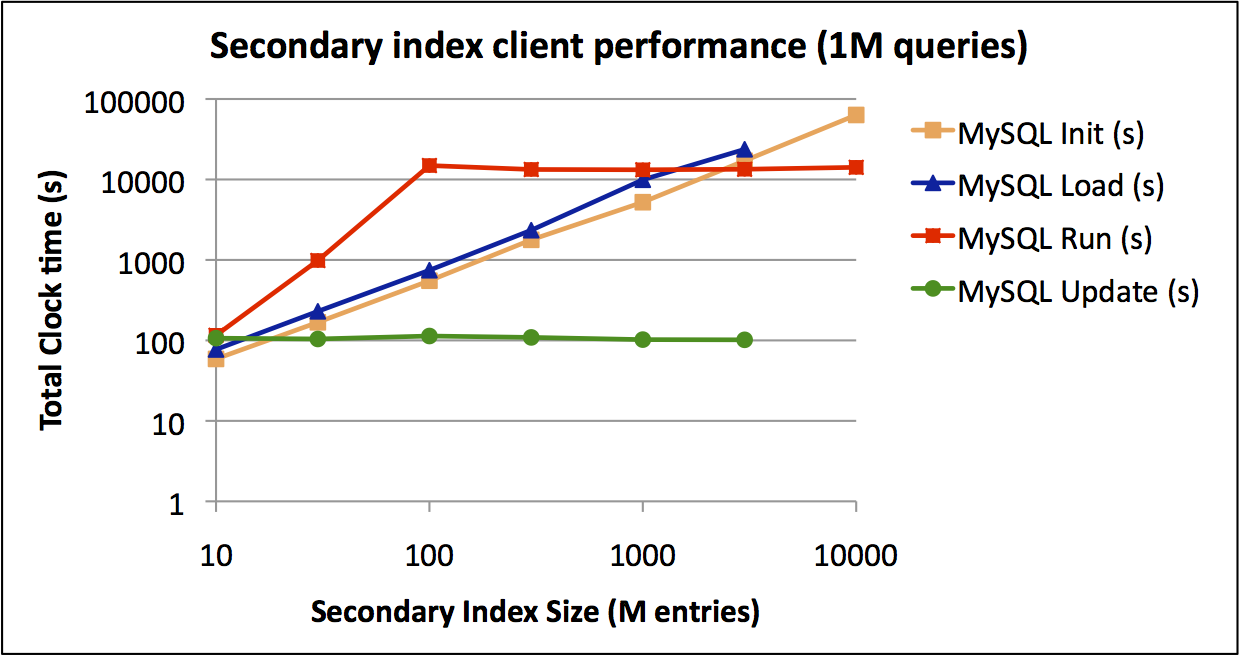
\includegraphics[width=\textwidth]{_static/indexing_tests.png}
\caption{Performance tests of MySQL-based secondary index.}
\end{figure}

To improve the performance of the InnoDB storage engine for queries, the
secondary index may be split across a small number (dozens) of tables,
each containing a contiguous range of keys. This splitting, if done,
will be independent of the partitioning of the database itself. The
contiguity of key ranges will allow the secondary index service to
identify the appropriate split table arithmetically via an in-memory
lookup.

\subsubsection{Secondary Index
Structure}\label{secondary-index-structure}

The secondary index consists of three columns: the key (objectId), the
chunk where all data with that key are located (chunkId), and the
subchunk within that chunk where data with the key are located
(subChunkId). The objectId is assigned by the science pipelines as a
64-bit integer value; the chunkId and subChunkId are both 16-bit
integers which identify spatial regions on the sky.

\subsubsection{Secondary Index Loading}\label{secondary-index-loading}

The InnoDB storage engine loads tables most efficiently if it is
provided input data which has been presorted according to the table's
primary key. When the secondary index information is collected for
loading (from each worker node handling a collection of chunks), it is
sorted by objectId, and may be divided into roughly equal ``splits''.
Each of those splits is loaded into a table \emph{en masse}.

To fully optimize the loading and table splitting, the entire index
should be collected from all workers and pre-sorted in memory on the
czar. This is not reasonable for 40 billion entries (requiring a minimum
of 480 GB memory, plus overhead). Instead, the index data from a single
worker can be assumed to be a ``representative sample'' from the full
range of objectIds, so table splitting can be done using the first
worker's index data. The remaining workers will be split and loaded
according to those defined tables.

\subsection{Data Distribution}\label{data-distribution}

LSST will maintain the released data store both on tape media and on a
database cluster. The tape archive is used for long-term archival. Three
copies of the compressed catalog data will be kept. The database cluster
will maintain 3 online copies of the data. Because computer clusters of
reasonable size failure regularly, the cluster must maintain replicas in
order to provide continuous data access. A replication factor of 3 (r=3)
is needed in order to determine data integrity by majority rule when one
replica is corrupt.

If periodic unplanned downtime is acceptable, an on-tape replica may
function as one of the three. However, the use of tape dramatically
increases the cost of recovering from a failure. This may be acceptable
for some tables, particularly those that are large and lesser-used,
although allowing service disruption may make it difficult to make
progress on long-running analysis on those large tables.

\subsubsection{Database data
distribution}\label{database-data-distribution}

The baseline database system will provide access for two database
releases: latest and previous . Data for each release will be spread out
among all nodes in the cluster.

Data releases are partitioned spatially, and spatial pieces (chunks) are
distributed in a round-robin fashion across all nodes. This means that
area queries involving multiple chunks are almost guaranteed to involve
resources on multiple nodes.

Each node should maintain at least 20\% free space of its data storage
allocation. The remaining free space is then available to be
``borrowed'' when another node fails. This will a temporary use of
storage capacity until more server resources can be put online, until
the 80\% storage use is returned.

\subsubsection{Failure and integrity
maintenance}\label{failure-and-integrity-maintenance}

There will be failures in any large cluster of node, in the nodes
themselves, in data storage volumes, in networks access and so on. These
failures will remove access to data that is resident on those nodes, but
this loss of data access should not affect that ability of scientists to
analyze the dataset as a whole. We need to set a data availability time
over 99.5\% to ensure confidence of the community in the stability of
the system. To ensure this level of data access, and to allow acceptable
levels of node failures in a cluster, there will be replication of data
on a table level throughout the cluster.

The replication level will be that each table in the database will exist
3 times, each on separate nodes. A monitoring layer to the system will
check on the availability of each table every few hours, although this
time will be tuned in practice. When this layer sees that a table has
less than three replicas available, this will initiate a replication of
that table to another nodes, not currently hosting that table. The times
for the checking, and speed of replication will be tuned to the
stability of the cluster, such that about 5\% of all tables at any given
time will only have 1 or 2 replicas. Three replicas will ensure that
tables will be available even in cases of large failures, or when nodes
need to be migrated to new hardware in bulk.

Should an entire node fail, replicating that data to another single node
would be fairly expensive in terms of time. As of July 2013, a 3TB drive
will have a write speed of 60/150/100 MB/s (min/max/avg),
{[}\url{http://www.legitreviews.com/article/2092/3/}{]} and refilling
this single drive would remove access to that replica of the data for
about 8 hours. We plan on having free space on each node, and only fill
local storage to 80\%. The free space will be used for temporary storage
of tables on failures, where replicas can take place in parallel between
nodes into this free space. When new nodes with free storage are added
to the cluster, then this data can be copied off this free space into
the drive, taking the full 8 hours, but there will still be 3 replicas
of data during this time. Once this is complete, this data will have 4
replicas for the short period of time while these tables can be removed
from the temporary storage, returning each node to 80\% usage.

\subsection{Metadata}\label{metadata}

Qserv needs to track various metadata information, static (not changing
or changing very infrequently), and dynamic (run-time) in order to
maintain schema and data integrity and optimize the cluster usage.

\subsubsection{Static metadata}\label{static-metadata}

Qserv typically works with databases and tables distributed across many
different machines: it breaks individual large tables into smaller
chunks and distributes them across many nodes. All chunks that belong to
the same logical table must have the same schema and partitioning
parameters. Different tables often need to be partitioned differently,
for example some tables might be partitioned with overlap (such as the
Object table), some might be partitioned with no overlap (for example
the Source table), and some might not need partitioning at all (e.g., a
tiny Filter table). Further, there might be different partitioning
strategies, such as spherical-box based, or HTM-based. All this
information about schema and partitioning for all Qserv-managed
databases and tables needs to be tracked and kept consistent across the
entire Qserv cluster.

Implementation of the static metadata in Qserv is based on hierarchical
key-value storage which uses a regular MySQL database as a storage
backend. This database is shared between multiple masters and it must be
served by a fault-taulerant MySQL server instance, e.g. using a
master-master replication solution like MariaDB Galera cluster. Database
consistency is critical for metadata and it should be implemented using
one of the transactional database engines in MySQL.

Static metadata may contain following information:

\begin{itemize}
\item
  Per-database and per-table partitioning and scan scheduling
  parameters.
\item
  Table schema for each table, used to create database tables in all
  worker and master instances; the schema in the master MySQL instance
  can be used to obtain the same information when a table is already
  created.
\item
  Database and table state information, used primarily by the process of
  database and table creation or deletion.
\item
  Definitions for the set of worker and master nodes in a cluster
  including their availability status.
\end{itemize}

The main clients of the static metadata are:

\begin{itemize}
\item
  Administration tools (command-line utilities and modules) which allow
  one to define or modify metadata structures.
\item
  Qserv master(s), mostly querying partitioning parameters but also
  allowed to modify table/database status when deleting/creating new
  tables and databases. Master(s) should not depend on node definitions
  in metadata, the xrootd facility is used to communicate with workers.
\item
  Special ``watcher'' service which implements distributed process of
  database and table management.
\item
  An initial implementation of the data loading application which will
  use the node definitions and will create/update database and table
  definitions. This initial implementation will eventually be replaced
  by a distributed loading mechanism which may be based on separate
  mechanisms.
\end{itemize}

\subsubsection{Dynamic metadata}\label{dynamic-metadata}

In addition to static metadata, a Qserv cluster also needs to track its
current state, and keep various statistics about query execution. This
sort of data is udated frequently, several times per query execution,
and is called dynamic metadata.

Prototype implementation of the dynamic metadata is based on MySQL
database. Like static metadata it needs to be shared between all master
instances and will be served via a single fault-talerant MySQL instance
which will be shared with static metadata database.

Dynamic metadata will contain the following information:

\begin{itemize}
\item
  Definition of every master instance in a Qserv cluster.
\item
  Record of every SELECT-type query processed by cluster. This record
  includes query processing state and some statistical/timing
  information.
\item
  Per-query list of table names used by the asynchronous queries, this
  information is used to delay table deletion while async queries are in
  progress.
\item
  Per-query worker information, which includes chunk id and identifying
  information for the worker processing that chunk id. This information
  will be used to transparently restart the master or migrate query
  processing to a different master in case of master failure.
\end{itemize}

The most significant use of the dynamic metadata is to track execution
of asyncronous queries. When an async query is submitted it is
registered in dynamic metadata and its ID is returned to the user
immediately. Later users can request status information for that query
ID which is obtained from dynamic metadata. When query processing is
finished users can request results from that query, and the master can
obtain the location of the result data from dynamic metadata.

Additionally dynamic metadata can be used to collect statistical
information about queries that were executed in the past which may be an
important tool in understanding and improving system performance.

\subsubsection{Architecture}\label{architecture}

The Qserv metadata system is implemented based on master/server
architecture: the metadata is centrally managed by a \emph{Qserv
Metadata Server} (qms). The information kept on each worker is kept to a
bare minimum: each worker only knows which databases it is supposed to
handle, all remaining information can be fetched from the qms (through
Qserv) as needed. This follows our philosophy of keeping the workers as
simple as possible.

The real-time metadata is managed inside qms in in-memory tables,
periodically synchronized with disk-based table. Such configuration
allows reducing qms latency---important to avoid delaying query
execution time. Should a qms failure occur, the in-flight queries for
which the information was lost will be restarted. Since the
synchronization to disk-based table will occur relatively frequently
(eg. at least 1 per minute), the lost time is insignificant. To avoid
overloading the qms with, only the high-level information available from
Qserv-master is stored in qms; all worker-based information is cached in
a scratch space locally to each worker in a simple, raw form (e.g,
key-value, ASCII file), and can be fetched on demand as needed.

At the moment we use xml-rpc as a message protocol to communicate with
qms. It was a natural choice given that this protocol is already in use
by Qserv master.

\subsubsection{Typical Data Flow}\label{typical-data-flow}

Static metadata:

\begin{enumerate}
\def\labelenumi{\arabic{enumi}.}
\item
  Parts of the static metadata known before data is partitioned/loaded
  are loaded by the administration scripts responsible for loading data
  into the database, then these scripts start data partitioner.
\item
  The data partitioner reads static metadata loaded by the
  administration scripts, loads remaining information.
\item
  When Qserv starts, it fetches all static metadata and caches it in
  memory in a special, in-memory optimized C++ structure.
\item
  The contents of the in-memory metadata cache inside Qserv can be
  refreshed on demand if the static metadata changes (for example, when
  a new database or a table is added).
\end{enumerate}

Dynamic-metadata:

\begin{enumerate}
\def\labelenumi{\arabic{enumi}.}
\item
  Master loads the information for each query (when it starts, when it
  completes).
\item
  Detailed statistics are dumped by each worker into a scratch space
  kept locally. This information can be requested from each worker on
  demand. A typical use case: if all chunk-queries except one completed,
  qms would fetch statistics for the still-running chunk-query to
  estimate when the query might finish, whether to restart this query
  etc.
\end{enumerate}

\subsection{Shared Scans}\label{shared-scans}

Arbitrary full-table scanning queries must be supported in LSST's
baseline catalog, and in order to provide this support cost-effectively
and efficiently, Qserv implements shared scans. Shared scans effectively
reduces the I/O cost of executing multiple scanning queries
concurrently, reducing the system hardware need and purchasing costs.

Shared scans reduce overall I/O costs by forcing incoming queries to
share. When multiple queries scan the same table, theoretically, they
can completely share I/O and incur only the I/O cost of a single query
rather than the sum of their individual costs. In general, it is
difficult for queries to share I/O because their arrival times are
random and uncorrelated. Each query begins scanning at different times,
and because LSST's catalog tables will be so large, general system
caching is ineffective. In Qserv, scanning queries are broken up into
many parts, and shared scanning forces each query to operate on the same
portion and thus share I/O cost, rather than allowing each to perform
its own ordered scan and incur costs individually.

\subsubsection{Background}\label{shared-scan-background}

Historically, shared scanning has been a research topic that has very
few real-world implementations. We know of only one implementation in
use (Teradata). Most database implementations assume OS or database
caching is sufficient, encouraging heavy use of indexing to reduce the
need of table scans. However, our experiments have shown that when
tables are large enough (by row count) and column access sufficiently
variable (cannot index enough columns when there are hundreds to choose
from), indexes are insufficient. With large tables, indexes no longer
fit in memory, and even when they do fit in memory, the seek cost to
retrieve each row is dominant when the index selects a percentage of
rows, rather than some finite number (thousands or less).

\subsubsection{Implementation}\label{shared-scan-implementation}

The implementation of shared scans in Qserv is in two parts. The first
part is a basic classification of incoming queries as scanning queries
or non-scanning queries. A query is considered to scan a table if it
depends on non-indexed column values and involves more than \emph{k}
chunks (where \emph{k} is a tunable constant). Note that involving
multiple chunks implies that the query selects from at least one
partitioned table. This classification is performed during query
analysis on the front-end and leveraging table metadata. The metadata
includes a ``scan rating'', which is set by hand. Higher scan ratings
indicate larger tables that take longer to read from disk. The
identified ``scan tables'' and their ratings are marked and passed along
to Qserv workers, which use the information in scheduling the fragments
of these scanning queries.

The second part of the shared scans implementation is a scheduling
algorithm that orders query fragment execution to optimize cache
effectiveness. Because Qserv relies on individual off-the-shelf DBMS
instances on worker nodes, it is not allowed to modify those instances
to implement shared scans. Instead, it issues query fragments ordered to
maximize locality of access in data and time, and tries to lock the
files associated with the tables in memory as much as possible. Using
the identified scan tables and their ratings, the worker places them on
the appropriate scheduler. There will be at least three schedulers. One
for queries expected to complete in under an hour, which are expected to
be related to the Object table. One for queries expected to take less
than eight hours, expected to be related to Object\_Extra. And one for
scans expected to take eight to twelve hours for ForcedSource and/or
Source tables. The reasoning being that a single slow query can impede
the progress of a shared scan and all the other user queries on that
scan. There may be a need for another scheduler to handle queries taking
more than 12 hours.

Each scheduler places incoming chunk queries into one of two priority
queues sorted by chunk id then scan rating of the individual tables. If
the query is for a chunk after the currently scanning chunk id, it is
placed on the active priority queue, otherwise it is placed on the
pending priority queue. After chunk id, the priority queue is sorted by
the table with highest scan rating to ensure that the largest tables in
the chunk are grouped together.

Once the query is on the appropriate scheduler, the algorithm proceeds
as follows. When a dispatch slot is available, it checks the highest
priority scheduler. If that scheduler has a query fragment, hereafter
called tasks, and it is not at its quota limit, it is allowed to start
its next task, otherwise the worker checks the next scheduler. It
continues doing this until a task has been started or all the schedulers
have been checked.

Each scheduler is only allowed to start a task under certain
circumstances. There must be enough threads available from the pool so
that none of the other schedulers are starved for threads as well as
enough memory available to lock all the tables for the task in memory.
If the scheduler has no tasks running, it may start one task and have
memory reserved for the tables in that task. This should prevent any
scheduler from hanging due to memory starvation without requiring
complicated logic but could incur extra disk I/O. More on locking tables
in memory later.

Schedulers check for tasks by first checking the top of the active
priority queue. If the active priority queue is empty, and the pending
priority queue is not, then the active and pending queues are swapped
with the task being taken from the top of the ``new'' active queue.

Since the queries are being run by a separate DBMS instance of which
there is little control of how it goes about running queries, the worker
can control when queries are sent to the DBMS and also lock files in
memory. Files in memory are among the most likely items to be paged out
when memory resources are low, which would increase disk I/O. Locking
files in memory prevents this from happening. However, care must taken
in choosing how much memory can be used for locking files. Use too much
and there will be a significant impact on DBMS performance. Set aside
too little, and schedulers will not make optimum use of the resources
available and may be forced to run tasks without actually locking the
files in memory.

The memory manager controls which files are locked in memory. When a
scheduler tries to run a task, the task asks the memory manager to lock
all the shared scan tables it needs. The memory manager determines which
files are associated with the tables. If the files are already locked in
memory and there is enough memory available to lock the files which are
not already locked, the task is given a handle and allowed to run. When
the task completes, it hands the handle back to the memory manager. If
it was the last task using any particular table, the memory for the
files used by that table is freed.

When the memory manager locks a file, it does not read the file. It only
sets aside memory for the file to occupy when it is read by the DBMS. In
the special case where a task can run even though there is not enough
memory available, those tables that cannot fit are put on a list of
reserved tables and their size is subtracted from the quota until they
can be locked or freed. When memory is freed, the memory manager will
try to lock the reserved tables.

Because Qserv processes interactive, short queries concurrently with
scanning queries, its query scheduler should be able to allow for those
queries to complete without waiting for a query scan. To achieve this,
Qserv worker nodes choose between the scan scheduler described above and
a simpler \emph{grouping} scheduler. Incoming queries with identified
scan tables are admitted to the scan scheduler, and all other queries
are admitted to the grouping scheduler. The grouping scheduler is a
simple scheduler that is a simple variant of a plain FIFO
(first-in-first-out) scheduler. Like a FIFO scheduler, it maintains a
queue of queries to execute, and operates identically to a FIFO
scheduler with one exception--queries are grouped by chunk id. Each
incoming query is inserted into the queue behind another query on the
same chunk, and at the back if no queued query matches. The grouping
scheduler assumes that the queue will never get very long, because it is
intended to only handle short interactive queries lasting fractions of
seconds, but groups its queue according to chunk id in order to provide
a minimal amount of access locality to improve throughput at a limited
cost to latency. Some longer queries will be admitted to the grouping
scheduler even though they are scanning queries, provided that they have
been determined to only scan a single chunk. Although these non-shared
scan query will disrupt performance of the overall scan on the
particular disk on a worker, the impact is thought to be small because
each of these represents all (or a large fraction of) the work for a
single user query, and the impact is amortized among all disks on all
workers.

For discussion about the performance of the existing prototype, refer to
demo-shared-scans.

\subsubsection{Memory management}\label{shared-scan-memory-management}

To minimize system paging when multiple threads are scanning the same
table, we implemented a memory manager called \href{}{memman}. When a
shared scan is about to commence, the shared scan scheduler informs
\href{}{memman} about the tables the query will be using and how
important it is to keep those tables in memory during the course of the
query. When directed to keep the tables in memory, \href{}{memman} opens
each data base table file, maps it into memory, and then locks the pages
to prevent the kernel from stealing the pages for other uses. Thus, once
a file page is faulted in, it stays in memory and allows other threads
to scan the contents of the page without incurring additional page
faults. Once the shared scan of the table completes, \href{}{memman} is
told that the tables no longer need to remain in memory. \href{}{memman}
frees up the pages by unlocking them and deleting the mapping.

This type of management is necessary to satisfy system paging
requirements because the prime paging pool is the set of unlocked file
system pages.

\subsubsection{\texorpdfstring{\href{http://xrootd.org}{XRootD}
scheduling
support}{XRootD scheduling support}}\label{shared-scan-xrootd-scheduling-support}

When the front-end dispatches a query, the
\href{http://xrootd.org}{XRootD} normally picks the least used server in
an attempt to spread the load across all of the nodes holding the
required table. While this works well for interactive queries, it is
hardly ideal for shared scan queries. In order to optimize memory and
I/O usage, queries for the same table in a shared scan should all be
targeted to the same node. A new scheduling mode was added to the
\href{http://xrootd.org}{XRootD} cmsd called affinity scheduling. The
front-end can tell \href{http://xrootd.org}{XRootD} whether or not a
particular query has affinity to other queries using the same table.
Queries that have affinity are always sent to the same node relative to
the table they will be using. This allows the back-end scheduler to
minimize paging by running the maximum number of queries against the
same table in parallel. Should that node fail,
\href{http://xrootd.org}{XRootD} assigns another working node that has
the table as the target node for queries that have affinity.

\subsubsection{Multiple tables support}\label{shared-scan-multiple-tables-support}

Handling multiple tables in shared scans requires an additional level of
management. The scheduler will aim to satisfy a throughput yielding
average scan latencies as follows:

\begin{itemize}
\item
  \texttt{Object} queries: 1 hour
\item
  \texttt{Object}, \texttt{Source} queries (join): 12 hours
\item
  \texttt{Object}, \texttt{ForcedSource} queries (join): 12 hours
\item
  \texttt{Object\_Extras}\footnote{This includes all
    \texttt{Object}-related tables, e.g., \texttt{Object\_Extra},
    \texttt{Object\_Periodic}, \texttt{Object\_NonPeriodic},
    \texttt{Object\_APMean}} queries (join): 8 hours.
\end{itemize}

As stated in 8.10.2, there will be schedulers for queries that are
expected to take one hour, eight hours, or twelve hours. The schedulers
group the the tasks by chunk id and then the highest scan rating of the
all tables in the task. The scan ratings are meant to be unique per
table and indicative of the size of the table, so that this sorting
places scans using the largest table from the same chunk next to each
other in the queue. Using scan rating allows flexibility to work with
data sets with schemas different than that of LSST.

Since scans are not limited to specific tables, complicated joins could
occur in user queries that could take more than twelve hours to process.
The worker may also need to be able to identify user queries that are
too slow for the current scheduler based on the time it takes to
complete tasks for that query. This indicates there may be a need for a
scheduler to handle queries with very long run times.

\subsection{Level 3: User Tables, External
Data}\label{level-3-user-tables-external-data}

Level 3 tables including tables generated by users, and data catalogs
brought from outside, depending on their type and size, will be either
partitioned and distributed across the production database servers, or
kept unpartitioned in one central location. While the partitioned and
distributed Level 3 data will share the nodes with Level 2 data, it will
be kept on dedicated disks, independent from the disks serving Level 2
data. This will simplify maintenance and recoverability from failures.

Level 3 tables will be tracked and managed through the Qserv Metadata
System (qms), described in the \emph{Metadata} chapter above. This
includes both the static, as well as the dynamic metadata.

\subsection{Cluster and Task
Management}\label{cluster-and-task-management}

Qserv delegates management of cluster nodes to
\href{http://xrootd.org}{XRootD}. The \href{http://xrootd.org}{XRootD}
system manages cluster membership, node registration/de-registration,
address lookup, replication, and communication. Its Scalable Service
Interface (\href{}{SSI}) API provides data-addressed communication
channels to the rest of Qserv, hiding details like node count, the
mapping of data to nodes, the existence of replicas, and node failure.
The Qserv manager focuses on dispatching queries to endpoints and Qserv
workers focus on receiving and executing queries on their local data.

Cluster management performed outside of \href{http://xrootd.org}{XRootD}
does not directly affect query execution, but include coordinating data
distribution, loading, nodes joining/leaving and is discussed in
qserve-admin. The \href{}{SSI} API includes methods that allow dynamic
updates to the data view of an \href{http://xrootd.org}{XRootD} cluster.
So that when new tables appear or disappear, the
\href{http://xrootd.org}{XRootD} system will incorporate that
information for future scheduling decisions. Thus, clusters can
dynamically change without the need to restart the
\href{http://xrootd.org}{XRootD} system.

\subsection{Fault Tolerance}\label{fault-tolerance}

Qserv approaches fault tolerance in several ways. The design exploits
the immutability of the underlying data by replicating and distributing
data chunks across a cluster such that in the event of a node failure,
the problem can be isolated and all subsequent queries re-routed to
nodes maintaining duplicate data. Moreover, this architecture is
fundamental to Qserv's incremental scalability and parallel performance.
Within individual nodes, Qserv is highly modularized with minimal
interdependence among its components, which are connected via narrow
interfaces. Finally, individual components contain specialized logic for
minimizing, handling, and recovering from errors.

The components that comprise Qserv include features that independently
provide failure-prevention and failure-recovery capabilities. The MySQL
proxy is designed to balance its load among several underlying MySQL
servers and provide automatic fail-over in the event a server fails. The
\href{http://xrootd.org}{XRootD} system provides multiple managers and
highly redundant servers to provide high bandwidth, contend with high
request rates, and cope with unreliable hardware. And the Qserv master
itself contains logic that works in conjunction with
\href{http://xrootd.org}{XRootD} to isolate and recover from
worker-level failures.

A worker-level failure denotes any failure mode that can be confined to
one or more worker nodes. In principle, all such failures are
recoverable given the problem nodes are identified and alternative nodes
containing duplicate data are available. Examples of such failures
include a disk failure, a worker process or machine crashing, or network
problems that render a worker unreachable.

Consider the event of a disk failure. Qserv's worker logic is not
equipped to manage such a failure on localized regions of disk and would
behave as if a software fault had occurred. The worker process would
therefore crash and all chunk queries belonging to that worker would be
lost. The in-flight queries on its local mysqld would be cleaned up and
have resources freed. The Qserv master's requests to retrieve these
chunk queries via \href{http://xrootd.org}{XRootD} would then return an
error code. The master responds by re-initializing the chunk queries and
re-submits them to \href{http://xrootd.org}{XRootD}. Ideally, duplicate
data associated with the chunk queries exists on other nodes. In this
case, \href{http://xrootd.org}{XRootD} silently re-routes the request(s)
to the surviving node(s) and all associated queries are completed as
usual. In the event that duplicate data does not exist for one or more
chunk queries, \href{http://xrootd.org}{XRootD} would again return an
error code. The master will re-initialize and re-submit a chunk query a
fixed number of times (determined by a parameter within Qserv) before
giving up, logging information about the failure, and returning an error
message to the user in response to the associated query.

Error handling in the event that an arbitrary hardware or software bug
(perhaps within the Qserv worker itself) causes a worker process or
machine to crash proceeds in the same manner described above. The same
is true in the event that network loss or transient
sluggishness/overload has the limited effect of preventing
\href{http://xrootd.org}{XRootD} from communicating with one or more
worker nodes. As long as such failures are limited to a finite number of
workers and do not extend to the Qserv master node,
\href{http://xrootd.org}{XRootD} is designed to record the failure and
return an error code. Moreover, if duplicate data exists on other nodes,
this will be registered within \href{http://xrootd.org}{XRootD}, which
will successfully route any subsequent chunk queries.

In the event of an unrecoverable error, the Qserv master is equipped
with a status/error messaging mechanism designed to both log detailed
information about the failure and to return a human-readable error
message to the user. This mechanism includes C++ exception handling
logic that encapsulates all of the master's interactions with
\href{http://xrootd.org}{XRootD}. If an unrecoverable exception occurs,
the master gracefully terminates the query, frees associated resources,
logs the event, and notifies the user. Qserv's internal status/error
messaging system also generates a status message and timestamp each time
an individual chunk query achieves a milestone. Such milestones include:
chunk query dispatch, written to \href{http://xrootd.org}{XRootD},
results read from \href{http://xrootd.org}{XRootD}, results merged, and
query finalized. This real-time status information provides useful
context in the event of an unrecoverable error.

Building upon the existing fault-tolerance and error handling features
described above, future work includes introducing a heart-beat mechanism
on worker nodes that periodically pings the worker process and will
restart it in the event it becomes unresponsive. Similarly, a master
monitoring process could periodically ping worker nodes and restart a
worker machine if necessary. We are also considering managing failure at
a per-disk level, but this would require research since
application-level treatment of disk failure is relatively rare. It
should also be possible to develop an interface for checking the
real-time status of queries currently being processed by Qserv by
leveraging its internally used status/error messaging mechanism.

\subsection{Next-to-database
Processing}\label{next-to-database-processing}

We expect some data analyses will be very difficult, or even impossible
to express through SQL language. This might be particularly useful for
time-series analysis. For this type of analyses, we will allow users to
execute their analysis algorithms in a procedural language, such as
Python. To do that, we will allow users to run their own code on their
own hardware resources co-located with production database servers.
Users then run queries on the production database which stream rows
directly from database cluster nodes to the user processing cluster,
where arbitrary code may run without endangering the production
database. This allows their incurred database I/O needs to be satisfied
using the database system's shared scanning infrastructure while
providing the full flexibility of running arbitrary code.

\subsection{Administration}\label{administration}

\subsubsection{Installation}\label{installation}

Qserv as a service requires a number of components that all need to be
running, and configured together. On the master node we require mysqld,
mysql-proxy, \href{http://xrootd.org}{XRootD}, cmsd, qserv metadata
service, and the qserv master process. On each of the worker nodes there
will also be the mysqld, cmsd, and \href{http://xrootd.org}{XRootD}
service. These major components come from the MySQL,
\href{http://xrootd.org}{XRootD}, and Qserv distributions. But to get
these to work together we will also require many more software package,
such as protobuf, lua, expat, libevent, python, zope, boost, java,
antlr, and so on. And many of these require more recent versions than
you are provided in most system distributions. We have an installation
layer, developed by SLAC, and LPC in Clermont-Ferrand, France in
collaboration, which will determine the packages, configure, compile and
install them in an automated process.

Currently, the Qserv installation procedure supports only the official
LSST platform--- RHEL6, and SL6 Linux distributions. Other UNIX-like
systems will be supported in the future as needed. The Qserv package
first can be downloaded from SLAC for install. In the initial README
there are basic install procedures, which start with a bootstrap script,
that will perform a yum install of needed packages distributed with
RHEL6, where the versions will support the Qserv install. Once that is
done an install script can be started. This will first download needed
packages not shipped with RHEL6 from SLAC, and get those installed
first. All software will be installed into a sandbox root path, and all
installed by the production username. Along with this is an install of
MySQL from source that will be configured for Qserv. These further
packages will be configured to run together, and then Qserv will be
complied and linked to these installed packages. All this runs without
user interaction, and usually completes within 15 to 20 minutes, to
provide a complete Qserv either master or worker node.

\subsubsection{Data loading}\label{data-loading}

As previously mentioned, Data Release Production will not write directly
to the database. Instead, the DRP pipelines will produce binary FITS
tables and image files that are reliably archived as they are produced.
Data will be loaded into Qserv in bulk for every table, so that tables
are either not available, or complete and immutable from the user query
access perspective.

For replicated tables, these FITS files are converted to CSV (e.g. by
harvesting FITS image header keyword value pairs, or by translating
binary tables to ASCII), and the resulting CSV files are loaded directly
into MySQL and indexed. For partitioned tables like Object and Source,
FITS tables are fed to the Qserv partitioner, which assigns partitions
based on sky coordinates and converts to CSV.

In particular, the partitioner divides the celestial sphere into
latitude angle ``stripes'' of fixed height H. For each stripe, a width W
is computed such that any two points in the stripe with longitudes
separated by at least W have angular separation of at least H. The
stripe is then broken into an integral number of chunks of width at
least W, so that each stripe contains a varying number of chunks (e.g.
polar stripes will contain just a single chunk). Chunk area varies by a
factor of about pi over the sphere. The same procedure is used to obtain
subchunks: each stripe is broken into a configurable number of
equal-height ``substripes'', and each substripe is broken into
equal-width subchunks. This scheme is preferred over the Hierarchical
Triangular Mesh for its speed (no trigonometry is required to locate the
partition of a point given in spherical coordinates), simplicity of
implementation, and the relatively fine control it offers over the area
of chunks and sub-chunks.

The boundaries of subchunks constructed as described are boxes in
longitude and latitude - the overlap region for a subchunk is defined as
the spherical box containing all points outside the subchunk but within
the overlap radius of its boundary.

The task of the partitioner is to find the IDs of the chunk and subchunk
containing the partitioning position of each row, and to store each row
in the output CSV file corresponding to its chunk. If the partitioning
parameters include overlap, then the row's partitioning position might
additionally fall inside the overlap regions of one or more subchunks.
In this case, a copy of the row is stored for each such subchunk (in
overlap CSV files).

Tables that are partitioned in Qserv must be partitioned identically
within a Qserv database. This means that chunk tables in a database
share identical partition boundaries and identical mappings of chunk id
to spatial partition. In order to facilitate table joining, a single
table's columns are chosen to define the partitioning space and all
partitioned tables (within a related set of tables) are either
partitioned according that pair of columns, or not partitioned at all.
Our current plan chooses the Object table's \texttt{ra\_PS} and
\texttt{decl\_PS} columns, meaning that rows in the Source and
ForcedSource tables will be partitioned according to the Objects they
reference.

There is one exception: we allow for pre-computed spatial match tables.
As an example, such a table might provide a many-to-many relationship
between the LSST Object catalog and a reference catalog from another
survey, listing all pairs of LSST Objects and reference objects
separated by less than some fixed angle. The reference catalog cannot be
partitioned by associated Object, as more than one Object might be
matched to a reference object. Instead, the reference catalog must be
partitioned by reference object position. This means that a row in the
match table might refer to an Object and reference object assigned to
different chunks stored on different Qserv worker nodes.

We avoid this complication by again exploiting overlap. We mandate (and
verify at partitioning time) that no match pair is separated by more
than the overlap radius. When partitioning match tables, we store a copy
of each match in the chunk of both positions referenced by that match.
When joining Objects to reference objects via the match table then, we
are guaranteed to find all matches to Objects in chunk C by joining with
all match records in C and all reference objects in C or in the overlap
region of C.

All Qserv worker nodes will partition subsets of the pipeline output
files in parallel -- we expect partitioning to achieve similar aggregate
I/O rates to those of full table scans for user query access, so that
partitioning should complete in a low factor (2-3x) of the table scan
time. Once it does, each Qserv worker will gather all output CSV files
for its chunks and load them into MySQL. The structure of the resulting
chunk tables is then optimized to maximize performance of user query
access (chunk tables will likely be sorted, and will certainly be
compressed), and appropriate indexes are built. Since chunks are sized
to fit in memory, all of these steps can be performed using an in-memory
file-system. I/O costs are incurred only when reading the CSV files
during the load and when copying finalized tables (i.e. .MYD/.MYI files)
to local disk.

The last phase of data loading is to replicate each chunk to one other
Qserv worker node. We will rely on table checksum verification rather
than a majority rule to determine whether a replica is corrupt or not.

The partitioner has been prototyped as a multi-threaded C++ program. It
uses an in-memory map-reduce implementation internally to scale across
cores, and can read blocks of one or more input CSV files in parallel.
It does not currently understand FITS table files. CSV file writes are
also parallelized - each output chunk is processed by a single reducer
thread and can be written to in parallel with no application level
locking. In preliminary testing, our partitioner was able to sustain
several hundred MB/s of both read and write bandwidth when processing a
CSV dump of the PT1.2 Source table.

We are investigating a pair of data loading optimizations. One is to
have pipeline processes either integrate the partitioning code or feed
data directly to the partitioner, rather than communicating via
persistent storage. The other is to write out tables in the native
database format (e.g. as .MYD files, ideally using the MySQL/MariaDB
server code to do so), allowing the CSV database loading step to be
bypassed.

\subsubsection{Administrative scripts}\label{administrative-scripts}

The administration of the qserv cluster will require a set of scripts,
all run from the one master machine, to control the large set of
workers. The main admin script, qserv-admin, will supply the base needs,
with starting all processes needed for the service, in order, and taking
down all processes to stop the service. Also base monitoring of service
is supplied here, to report on processes that are running, and
responding to base queries, to check on MySQL or
\href{http://xrootd.org}{XRootD} dying or locking up. Also is supplied
is the updating of the configuration definitions from the master out to
all workers, such that all machines need to have the same configurations
for the services.

The base data loading onto the nodes tends to be a slightly detailed
process, beyond the just the data preparation. Up to now, data
preparation produces text files in csv format, and then these will be
loaded into the MySQL layer as a MyISAM table. The schema for these
tables will need to have added to them the fields for chunk and subchunk
number needed for the Qserv service. The modification of the schema and
the control of the loading of the data, which can take hours, is done
with the qserv-load script. The loading of the data is also done without
index creation, and then that is done after the data loading. We are
also experimenting with the use of compressed read-only tables for the
data serving, and this is an option.

Another needed setup for the data service in qserv, is the creation of
the ``emptyChunks'' list. The data will be spatially partitioned into
``chunks'', as previously described, but the for the complete service,
the master process with need to know how many chunks exist in the data,
and which of these chunks contain no data. In queries which will involve
a complete table scan, which chunks to create query, or not, will need
to be known. Once the data is loaded, there is a another script which
will go out to nodes and see what chunks are there, and compile a list
of all possible chunks and which chunks do not contain data, or the
``emptyChunks'' lists. This is loaded by the qserv master process at
startup.

\subsection{Result Correctness}\label{result-correctness}

To verify Qserv does not introduce any unexpectedly alter results (e.g.,
does not show the same object twice or does not miss any objects on the
chunk boundaries), we developed an automated testbed, which allows us to
run pre-set queries on pre-set data sets both through plain MySQL and
through Qserv, and compare results.

\subsection{Current Status and Future
Plans}\label{current-status-and-future-plans}

As of now (June 2013) we have implemented a basic version of the system
end-to-end. Our prototype is capable of parsing a wide range of queries,
including queries executed by our QA system, ``PipeQA'', rewriting them
into sub-queries, executing these sub-queries in parallel and returning
results to the user. The implementation includes a generic parser, basic
query scheduler, job executor, query result collector. We demonstrated
running all query types (low, high, super-high such as large-area
near-neighbor) including aggregations, scalably on a 150-node cluster
using 30 TB data set; and a smaller subset of queries scalably on
300-node cluster (remaining tests in progress, expecting to complete in
the next 2-3 weeks) we also demonstrated the system performs well enough
to meet the LSST query response time requirements. We demonstrated the
system can handle high-level of concurrency (10 concurrent queries
simultaneously accessing 10,000 chunks each). We demonstrated the system
can recover from a variety of faults, or at minimum gracefully fail if
the error is unrecoverable. We extended SQL syntax coverage and ensured
the system is capable of supporting all types of queries executed over
the course of recent data challenges by PipeQA and users. We implemented
a core foundation for the metadata, currently used for managing static
metadata about Qserv-managed databases and tables, a set of
administrative tools, and scalable data partitioner. We made the system
easy to set up, resilient to typical failures and common user mistakes.
We implemented automated test bed. We consider the current prototype to
have a quality of a typical late-alpha / early-beta software.

Future work includes:

\begin{itemize}
\item
  extending metadata to support run-time statistics, implementing query
  management tools
\item
  implementing support for Level 3 data
\item
  completing initial shared scan implementation, testing and
  implementing concurrent and synchronized shared scans on multiple
  spindles
\item
  demonstrating cross-match with external catalogs
\item
  improving interfaces for users (eg hiding internal tables)
\item
  re-examining and improving query coverage, including more advanced SQL
  syntax, such as sub-queries as needed
\item
  improvements to administration scripts
\item
  support for HTM partitioning in Qserv
\item
  authentication and authorization
\item
  resource management
\item
  early partition results
\item
  performance improvements
\item
  partition granularity varying per table
\item
  security
\end{itemize}

\textbf{Extending metadata to support run-time statistics, implementing
query management tools}. Qserv currently does not maintain any explicit
run-time system state. Keeping such state would simplify managing Qserv
cluster, and building features such as query management: currently there
are no tools for inspecting and managing queries in-flight, and there
are no interfaces for halting queries except upon error detection. It is
clear that users and administrators will need to list running queries,
check query status and possibly abort queries.

\textbf{Implementing support for Level 3 data}. Qserv will need to
support level 3. That means users should be able to maintain their own
tables to store their own data or results from previous queries. They
should be able to create, drop, and update their own tables within the
system.

\textbf{Completing initial shared scan implementation, testing and
implementing concurrent and synchronized shared scans on multiple
spindles.} The first prototype implementation of shared scanning is
mostly complete, with the remaining work focused on basic analysis and
characterization of incoming user queries to determine scanning tables
and plumbing to convey the appropriate hints to worker nodes.

\textbf{Demonstrating cross-match with external catalogs}. One of the
use cases involves cross matching with external catalogs. In case the
catalogs to cross-match with is small, it will be treated as a small
table and replicated as metadata tables will be. For cross-matching with
larger catalogs, the catalog to cross-match with will need to be
partitioned and distributed on the worker nodes.

\textbf{Improving interfaces for users}. Many admin-type commands such
as ``list processes'' or ``explain'' are not ported to the distributed
Qserv architecture, and thus will not show correct result. At the moment
we have disabled these commands. Additionally, commands such as listing
tables in a given database will have to be overloaded, for example, we
should show user a table ``Object'' (even though in practice such table
does not exist in the Qserv system), instead of all the chunk
\texttt{Object\_XXX} tables, that are internal, and should not be
exposed to the end-user.

\textbf{Re-examining and improving query coverage, including more
advanced SQL syntax, such as sub-queries as needed}. We examined what
queries users and production processes execute, however we realize this
query set is far from the complete list of queries we will see in the
future. All needed syntax needs to be understood and fully supported.
Design and feasibility evaluation for sub-query support. Qserv does not
support SQL sub-queries. Since there is evidence that such a capability
might be useful to users, so we should formulate a few possible designs
and understand how easy/difficult they would be to implement. Note that
there are some alternative viable alternatives, such as splitting
sub-queries into multiple queries, and/or using session variables. A
naïve implementation that involves dumping all sub-query results to disk
and then reading these results from disk, similarly to how multiple
map/reduce stages are implemented, should be tractable to implement.

\textbf{Improvements to administration scripts}. To further automate
common tasks related to database management, table management, partition
management, data distribution, and others we need to implement many
improvements to the administration scripts.

\textbf{Support for HTM partitioning in Qserv}. HTM is an alternative to
the rectangular box form of spatial partitioning currently implemented
in Qserv. Since HTM allows for more advanced indexing and optimization,
it may eventually replace the current partitioning algorithm.

\textbf{Authentication and authorization}. The current Qserv does not
implement any form of security or privileges. All access is full access.
A production database system should provide some facility of user or
role-based access so that usage can be controlled and resources can be
shared. This is in particular needed for Level-3 data products.

\textbf{Resource management}. A production system should have some way
to manage/restrict resource usage and provide quality-of-service
controls. This includes a monitoring facility that can track each node's
load and per-user-query resource usage.

\textbf{Early partition results}. When performing interactive
exploration of an observational data set, users frequently issue
large-scale queries that produce undesired results, even after testing
such queries on small subsets of the data. We can ameliorate this
behavior by providing the investigator with early partial results from
the query, allowing the user to recognize that the returned values are
incorrect and permitting the query to be aborted without wasting
additional resources. There are two mechanisms we will implement in
Qserv for providing early results. First, for queries that retrieve a
filtered set of rows, matching rows can be returned as their query
fragments complete, well before all fragments finish. Second, for
queries that group, sort, or aggregate information and therefore perform
a global operation after any per-partition processing, the global
operation can be applied to increasingly large subsets of the
per-partition results, returning an early partial result each time.

\textbf{Performance improvements}. Significant performance gain can be
obtained by improving scheduler. These improvements pose interesting
state of the art computing challenges; more details are available in
Appendix D. In addition, some parts of Qserv are inefficient since they
were implemented under constraints of development time rather than
efficiency, or maintainability -- rewriting them would result in further
performance gains. Caching results for future queries is another example
of performance optimization that can yield significant speed
improvements.

\textbf{Partitioning granularity varying per table}. Since large tables
in LSST vary significantly in row count and row size, it may be
worthwhile to support partitioning with multiple granularities. For
execution management it is useful to have partitions sized so that query
fragments have similar execution cost. To achieve this, partitions may
need different spatial sizes.

\textbf{Security}. The system needs to be secure and resilient against
denial of service attacks.

\subsection{Open Issues}\label{open-issues}

What follows is a (non-exhaustive) list of issues, technical and
scientific, that are still being discussed and where changes are
possible.

\begin{itemize}
\item
  \textbf{Support for updates}. Size of Level 1 catalog is relatively
  small, and the expected query access patterns are relatively
  non-challenging, thus currently do not envision any need to deploy
  scalable Qserv-like architecture for Alert Production. Should this
  change, we will need to support updates in Qserv, which will likely
  have some non-trivial impact on the architecture.
\item
  \textbf{Very large objects}. Some objects (eg, large galaxies) are
  much larger than our overlap region, in some cases their footprint
  will span multiple chunks. Currently we are working with the object
  center, neglecting the actual footprint. While there are some science
  use cases that would benefit from a system that tracks objects based
  on their footprint, this is currently not a requirement. Potential
  solution would involve adding a custom index similar to the
  r-tree-based indexes such as the TOUCH {[}67{]}.
\item
  \textbf{Very large results}. Currently, the front-end that disptached
  the query is responsible for assembling the results. In general, this
  is not a scalable approach as the resources required to processes the
  results may be several orders of magnitude greater than those needed
  to dispatch the query. One solution is to replicate the front-end to
  the extent necessary to handle query results. Alternatively, the
  Scalable Service Interface can be augmented to allow running
  disconnected queries. That is, once a particular front-end dispatches
  a query it can get a handle to that query and disconnect from it.
  Another server can, using that handle, reconnect to the query and
  process the results. This is a more flexible model as it allows
  independent scaling of query dispatch and result processing. It also
  has the aded benefit of not cancelling in-progress queries dispatched
  by a particulr fron-end should that front-end die.
\end{itemize}

\section{Large-scale Testing}\label{large-scale-testing}

\subsection{Introduction}\label{introduction-1}

\subsubsection{Ideal environment}\label{ideal-environment}

Based on the detailed spreadsheet analysis, we expect the ultimate LSST
production system will be composed of few hundred database servers
{[}LDM-144{]}\_, so a realistic test should include a cluster of at
least 100 nodes.

Total database size of a single data release will vary from
\textasciitilde{}1.3 PB (DR1) to \textasciitilde{}15 PB
(DR11).\footnote{These numbers are for single copy, data and indices,
  compressed when appropriate.} Realistic testing requires at least
\textasciitilde{}20-30 TB of storage (across all nodes).

Note that \emph{a lot} of highly focused tests which are extremely
useful to fine tune different aspects of the system can be done on a
very small, 2-3 cluster, or even on a single machine. An example of that
can be measuring the effect of table size on the performance of
near-neighbor join: this type of join will be done per sub-partition,
and sub-partitions will be small (few K rows), thus almost all tests
involving a single sub-partition can be done on a single machine with
very little disk storage.

A significant amount of testing should be done where the dataset size
exceeds the system memory size by an order of magnitude. This testing is
important to reveal system performance in the presence of disk
performance characteristics.

It is essential to have at least two different types of catalogs: Object
and Source. Of course this data needs to be correlated, that is, the
objects should corresponds to the sources. Having these 2 tables will
allow us to measure speed of joins. It is not necessary to have other
types of source-like tables (DiaSource, ForcedSource) -- the tests done
with Source should be a good approximation.

The most important characteristic of the test data is its spatial
distribution. The data should reflect realistic densities: presence of
very crowded or very sparse regions have influence on how data is
partitioned and on performance of certain queries (e.g., speed of near
neighbor inside one partition). Other than realistic spatial
distribution, we need several fields to be valid (e.g., magnitudes) in
order to try some queries with predicates.

These tests are not only used to prove our system is capable of meeting
the requirements, but also as a mean to stress the system and uncover
potential problems and bottlenecks. In practice, whoever runs these
tests should well understand the internals of the scalable architecture
system and turning MySQL.

\subsubsection{Schedule of testing}\label{schedule-of-testing}

\begin{itemize}
\item
  Selecting the base technology -- Q2 2009
\item
  Determining the architecture -- Q3 2009
\item
  Pre-alpha tests focused on parallel distributed query execution
  engine, tests at small scale (\textasciitilde{}20 nodes) -- Q4 2009
\item
  Most major features in (except shared scan, user tables), performance
  tests on mid-size cluster (\textasciitilde{}100 nodes) -- Q4 2010
\item
  Scalability and performance improvements and tests on a large cluster
  (150-250 nodes) -- Q4 2011
\item
  Large scale tests, performance tests on a large cluster (250-300
  nodes) -- Q2 2013
\item
  Shared scans -- Q3 2013
\item
  Fault tolerance -- Q4 2013
\end{itemize}

\subsubsection{Current status of tests}\label{current-status-of-tests}

We have run several large scale tests

\begin{enumerate}
\def\labelenumi{\arabic{enumi}.}
\item
  (10/2009) A test with the ``pre-alpha'' version of our software
  written on top of MySQL, using the \emph{Tuson} cluster at LLNL (160
  nodes, each node: two Intel Xeon 2.4 GHz GPUs with 4 GB RAM and 1
  local hard disk of 80 Gbs)
\item
  (2010) several 100-node tests run at SLAC {[}58{]}. These tests helped
  us uncover many bottlenecks and prompted rewriting parts of our
  software, as well as implementing several missing features in
  \href{http://xrootd.org}{XRootD}.
\item
  (4/2011) A 30 TB test on 150-node SLAC cluster using Qserv in
  40/100/150 node configurations, using 2 billion row Object and 32
  billion row Source tables, total of 30 TB data set.
\item
  (12/2012) A 100-terabyte test on JHU's \emph{Datascope} 20-node
  cluster. Due to high instability of the cluster this test turned into
  testing resilience to faults of Qserv and the associated
  administrative tools.
\item
  (05/2013) A 10,000-chunk test on a 120-node SLAC cluster to reproduce
  and understand subtle issues with concurrency at scale.
\item
  (07/2013) A test on 300-node IN2P3 cluster to re-test scalability,
  performance, concurrency, and uncover unexpected issues and
  bottlenecks.
\item
  (08/2013) A demonstration of shared scans.
\end{enumerate}

The tests 3-6 listed above are described in further details below.

\subsection{150-node Scalability Test}\label{node-scalability-test}

\subsubsection{Hardware}\label{hardware}

We configured a cluster of 150 nodes interconnected via gigabit
Ethernet. Each node had 2 quad-core Intel Xeon X5355 processors with
16GB memory and one 500GB 7200RPM SATA disk. Tests were conducted with
Qserv SVN r21589, MySQL 5.1.45 and \href{http://xrootd.org}{XRootD}
3.0.2 with Qserv patches.

\subsubsection{Data}\label{data}

We tested using a dataset synthesized by spatially replicating the
dataset from the LSST data challenge (``PT1.1''). We used two tables:
Object and Source.\footnote{The schema may be browsed online at
  \url{http://lsst1.ncsa.uiuc.edu/schema/index.php?sVer=PT1_1}} These
two tables are among the largest expected in LSST. Of these two, the
Object table is expected to be the most frequently used. The Source
table will have 50-200X the rows of the Object table, and its use is
primarily confined to time series analyses that generally involve joins
with the Object table.

The PT1.1 dataset covers a spherical patch with right-ascension between
358˚ and 5˚ and declination between -7˚ and 7˚. This patch was treated
as a spherical rectangle and replicated over the sky by transforming
duplicate rows' RA and declination columns, taking care to maintain
spatial distance and density by a non-linear transformation of
right-ascension as a function of declination. This resulted in an Object
table of 1.7 billion rows (2TB) and a Source table of 55 billion rows
(30 TB).\footnote{Source for the duplicator is available at
  \url{http://dev.lsstcorp.org/trac/browser/DMS/qserv/master/trunk/examples}}
The Source table included only data between -54˚ and +54˚ in
declination. The polar portions were clipped due to limited disk space
on the test cluster. Partitioning was set for 85 stripes each with 12
sub-stripes giving a $\phi$ height of \textasciitilde{}2.11˚ for stripes and
0.176˚ for sub-stripes. Each chunk thus spanned an area of approximately
4.5deg\textsuperscript{2}, and each sub-chunk,
0.031deg\textsuperscript{2}. This yielded 8,983 chunks. Overlap was set
to 0.01667˚ (1 arc-minute).

\subsubsection{Queries}\label{queries}

The current Qserv development focus is on features for scalability. We
have chosen a set of test queries that demonstrate performance for both
cheap queries (interactive latency), and expensive queries (hour, day
latency). Runs of low volume queries ranged from 15 to 20 queries, while
runs of high volume queries and super high volume queries consisted of
only a few or even one query due to their expense. All reported query
times are according to the command-line MySQL client (\emph{MySQL}).

\paragraph{Low-volume 1 -- object
retrieval}\label{low-volume-1-object-retrieval}

\begin{lstlisting}[language=SQL]
SELECT * FROM Object WHERE objectId = <objId>
\end{lstlisting}

In fig-150-node-low-vol-object-retrieval we can see that performance of
this query is roughly constant, taking about 4 seconds. Each run
consisted of 20 queries. The slower performance of Runs 1 and 4, where
each execution took 9 seconds, were probably the result of competing
tasks in the cluster. We attribute the initial 8 second execution time
in Run 5 and beyond to cold cache conditions (likely the objectId index)
in the cluster.

\begin{figure}[H]
\centering
\includegraphics{_static/150_node_low_vol_object_retrieval.png}
\caption{Low-volume object retrival.}
\end{figure}

\paragraph{Low-volume 2 -- time series}\label{low-volume-2-time-series}

\begin{lstlisting}[language=SQL]
SELECT taiMidPoint, fluxToAbMag(psfFlux), fluxToAbMag(psfFluxErr), ra, decl
FROM Source
WHERE objectId = <objId>
\end{lstlisting}

This query retrieves information from all detections of a particular
astronomical object, effectively providing a time-series of measurements
on a desired object. For testing, the objectId was randomized as for the
Low Volume 1 query, which meant that null results were retrieved where
the Source data was missing due to available space on the test cluster.

In fig-low-volume-time-series we see that performance is roughly
constant at about 4 seconds per query. Run 1 was done after Low Volume
1's Run 1 and we discount its 9 second execution times similarly as
anomalous.

\begin{figure}[H]
\centering
\includegraphics{_static/low_volume_time_series.png}
\caption{Low-volume time series.}
\end{figure}

\paragraph{Low-volume 3 -- spatially-restricted
filter}\label{low-volume-3-spatially-restricted-filter}

\begin{lstlisting}[language=SQL]
SELECT COUNT(*)
FROM Object
WHERE ra_PS BETWEEN 1 AND 2
AND decl_PS BETWEEN 3 AND 4
AND fluxToAbMag(zFlux_PS) BETWEEN 21 AND 21.5
AND fluxToAbMag(gFlux_PS)-fluxToAbMag(rFlux_PS) BETWEEN 0.3 AND 0.4
AND fluxToAbMag(iFlux_PS)-fluxToAbMag(zFlux_PS) BETWEEN 0.1 AND 0.12;
\end{lstlisting}

In fig-low-volume-spatial-filter we see the same 4 second performance
that was seen for the other low volume queries. Again, the
\textasciitilde{}9 second performance in Run 2 could not be reproduced
so we discount it as resulting from competing processes on the cluster.

\begin{figure}[H]
\centering
\includegraphics{_static/low_volume_spatial_filter.png}
\caption{Low-volume spatially-restricted filter.}
\end{figure}

\paragraph{High volume 1 -- count}\label{high-volume-1-count}

\begin{lstlisting}[language=SQL]
SELECT COUNT(*) FROM Object
\end{lstlisting}

\begin{figure}[H]
\centering
\includegraphics{_static/150_node_high_volume_count.png}
\caption{High volume count.}
\end{figure}

\paragraph{High-volume 2 -- full-sky
filter}\label{high-volume-2-full-sky-filter}

\begin{lstlisting}[language=SQL]
SELECT objectId, ra_PS, decl_PS, uFlux_PS, gFlux_PS,
       rFlux_PS, iFlux_PS, zFlux_PS, yFlux_PS
FROM Object
WHERE fluxToAbMag(iFlux_PS) - fluxToAbMag(zFlux_PS) > 4
\end{lstlisting}

Using the on-disk data footprint (MySQL's MyISAM .MYD, without indexes
or metadata) of the Object table (1.824x10\textsuperscript{12} bytes),
we can compute the aggregate effective table scanning bandwidth. Run 3's
7 minute execution yields 4.0GB/s in aggregate, or 27MB/s per node,
while the other runs yield approximately 11GB/s in aggregate, or 76MB/s
per node. Since each node was configured to execute up to 4 queries in
parallel, Run 3's bandwidth is more realistic, given seek activity from
competing queries and the disk manufacturer's reported theoretical
transfer rate of 98MB/s.

\begin{figure}[H]
\centering
\includegraphics{_static/150_node_high_volume_full_sky.png}
\caption{High volume full-sky filter.}
\end{figure}

\paragraph{High-volume 3 -- density}\label{high-volume-3-density}

\begin{lstlisting}[language=SQL]
SELECT COUNT(*) AS n, AVG(ra_PS), AVG(decl_PS), chunkId
FROM Object
GROUP BY chunkId
\end{lstlisting}

\begin{figure}[H]
\centering
\includegraphics{_static/150_node_high_volume_density.png}
\caption{High volume full-sky filter.}
\end{figure}

This query computes statistics for table fragments (which are roughly
equal in spatial area), giving a rough estimate of object density over
the sky. It illustrates more complex aggregation query support in Qserv.
This query is of similar complexity to High Volume 2, but
fig-150-node-high-volume-density illustrates measured times
significantly faster, which is probably due to reduced results
transmission time. As mentioned for HV2, cache behavior was not
controlled, but the 4 minute time in Run 3 may be close.

\paragraph{Super-high-volume 1 -- near
neighbor}\label{super-high-volume-1-near-neighbor}

\begin{lstlisting}[language=SQL]
SELECT COUNT(*)
FROM Object o1, Object o2
WHERE qserv_areaspec_box(-5,-5,5,-5)
AND qserv_angSep(o1.ra_PS, o1.decl_PS,
                 o2.ra_PS, o2.decl_PS) < 0.1
\end{lstlisting}

This query finds pairs of objects within a specified spherical distance
which lie within a particular part of the sky. Over two randomly
selected 100 deg\textsuperscript{2} areas, the execution times were
about 10 minutes (667.19 seconds and 660.25 seconds). The resultant row
counts ranged between 3 to 5 billion. Since execution uses on-the-fly
generated tables, the tables do not fit in memory, and Qserv does not
yet implement caching, we expect caching effects to be negligible.

\paragraph{Super-high-volume 2 -- sources not near
objects}\label{super-high-volume-2-sources-not-near-objects}

\begin{lstlisting}[language=SQL]
SELECT o.objectId, s.sourceId, s.ra, s.decl,
       o.ra_PS, o.decl_PS
FROM Object o, Source s
WHERE qserv_areaspec_box(224.1, -7.5, 237.1, 5.5)
AND o.objectId = s.objectId
AND qserv_angSep(s.ra, s.decl, o.ra_PS, o.decl_PS) > 0.0045
\end{lstlisting}

This is an expensive query -- an \(O(kn)\) join over 150 square degrees
between a 2TB table and a 30TB table. Each objectId is unique in Object,
but is shared by 41 rows (on average) in Source, so \(k
\sim 41\). We recorded times of a few hours (5:20:38.00, 2:06:56.33, and
2:41:03.45). The variance is presumed to be caused by varying spatial
object density over the three random areas selected.

\subsubsection{Scaling}\label{scaling}

We tested Qserv's scalability by measuring its performance while varying
the number of nodes in the cluster. To simulate different cluster sizes,
the frontend was configured to only dispatch queries for partitions
belonging to the desired set of cluster nodes. This varies the overall
data size proportionally without changing the data size per node
(200-300GB). We measured performance at 40, 100, and 150 nodes to
demonstrate weak scaling.

\paragraph{Scaling with small queries}\label{scaling-with-small-queries}

From fig-150-node-scaling-small-1 --- fig-150-node-scaling-small-3, we
see that execution time is unaffected by node count given that the data
per node is constant. The spike in the 40-node configuration in
fig-150-node-scaling-small-3 is caused by 2 slow queries (23s and 57s);
the other 28 executed in times ranging from 4.09 to 4.11 seconds.

\begin{figure}[H]
\centering
\includegraphics{_static/150_node_scaling_small_1.png}
\caption{Scaling with node count (1).}
\end{figure}

\begin{figure}[H]
\centering
\includegraphics{_static/150_node_scaling_small_2.png}
\caption{Scaling with node count (2).}
\end{figure}

\begin{figure}[H]
\centering
\includegraphics{_static/150_node_scaling_small_3.png}
\caption{Scaling with node count (3).}
\end{figure}

\paragraph{Scaling with expensive
queries}\label{scaling-with-expensive-queries}

\textbf{High Volume}

If Qserv scaled perfectly linearly, the execution time should be
constant when the data per node is constant. In
fig-150-node-scaling-high-volume the times for high volume queries show
a slight increase. HV1 is a primarily a test of dispatch and result
collection overhead and its time increases linearly with the number of
chunks since the front-end has a fixed amount of work to do per chunk.
Since we varied the set of chunks in order to vary the cluster size, the
execution time of HV1 should thus vary linearly with cluster size. HV3
seems to have a similar trend since due to cache effects -- its result
was cached so execution became more dominated by overhead.

The High Volume 2 query approximately exhibits the flat behavior that
would indicate perfect scalability. Caching effects may have clouded the
results, but they did not dominate. If the query results were perfectly
cached, we expect the overall execution time to be dominated by overhead
as in HV1, and this is clearly not the case.

\begin{figure}[H]
\centering
\includegraphics{_static/150_node_scaling_high_volume.png}
\caption{Scaling with high volume queries.}
\end{figure}

\textbf{Super High Volume}

The tests on expensive queries did not show perfect scalability, but
nevertheless, the measurements did show some amount of parallelism. It
is unclear why execution in the 100-node configuration was the slowest
for both SHV1 and SHV2. Our time-limited access to the cluster did not
allow us to repeat executions of these expensive queries and study their
performance in better detail.

\begin{figure}[H]
\centering
\includegraphics{_static/150_node_super_high_volume.png}
\caption{Scaling with super high volume queries.}
\end{figure}

\subsubsection{Concurrency}\label{concurrency}

\begin{figure}[H]
\centering
\includegraphics{_static/150_node_concurrency.png}
\caption{Concurrency test.}
\end{figure}

We were able to test Qserv with multiple queries in flight. We ran 4
``streams'' of queries: two parallel invocations of HV2, one of LV1, and
one of LV2. Each low volume stream paused for 1 second between queries.
Figure 12 illustrates concurrent performance. We see that the HV2
queries take about twice the time (5:53.75 and 5:53.71) as they would if
running alone. This makes sense since each is a full table scan that is
competing for resources and shared scanning has not been implemented.
The first queries in the low volume streams execute in about 30 seconds,
but each of their second queries seems to get ``stuck'' in queues. Later
queries in the streams finish faster. Since the worker nodes maintain
first- in-first-out queues for queries and do not implement any concept
of query cost, long queries can easily hog the system. The slowness of
low volume queries after the second queries may be curious at first
glance, since they should be queued at the end on their assigned worker
nodes and thus complete near the end of the HV2 queries. In that case,
subsequent queries would land on workers with nearly empty queues and
execute immediately. This slowness can be explained by query skew --
short queries may land on workers that have or have not finished their
work on the high volume queries.

\subsubsection{Discussion}\label{discussion-1}

\paragraph{Latency}\label{latency}

LSST's data access needs include supporting both small, frequent,
interactive queries and longer, hour/day-scale queries. We designed
Qserv to operate efficiently in both cases to avoid needing multiple
systems, which would be costly in development, maintenance, and
hardware. Indexing was implemented in order to reduce latency for cheap
queries that only touch a small part of the data.

The current Qserv implementation incurs significant overhead in
dispatching queries and collecting results. In early development we
decided to minimize the intelligence on each worker, so the front-end
master became responsible for preparing the SQL queries so that workers
did not need to perform parsing or variable substitution. Results
collection is somewhat heavyweight as well. MySQL does not provide a
method to transfer tables between server instances, so tables are dumped
to SQL statements using \emph{mysqldump} and reloaded on the front-end.
This method was chosen to speed prototyping, but its costs in speed,
disk, network, and database transactions are strong motivations to
explore a more efficient method.

\paragraph{Solid-state storage}\label{solid-state-storage}

Some of Qserv's design choices (e.g., shared scanning) are motivated by
the need to work around poor seek performance characteristics of disks.
Solid-state storage has now become a practical alternative to mechanical
disk in many applications. While it may be useful for indexes, its
current cost differential per unit capacity means that it is still
impractical to store bulk data. In the case of flash storage, the most
popular solid-state storage technology, shared scanning is still
effective in optimizing performance since DRAM is much faster than flash
storage and flash still has ``seek'' penalty characteristics (though it
is much better than spinning disk).

\paragraph{Many core}\label{many-core}

We expect the performance to be I/O constrained, since the workload is
data, not CPU performance limited. It is unlikely that many cores can be
leveraged on a single node since they will be sized with only the number
of disk spindles that saturate the north bridge, but shared scanning
should increase CPU utilization efficiency.

\paragraph{Alternate partitioning}\label{alternate-partitioning}

The rectangular fragmentation in right ascension and declination, while
convenient to visualize physically for humans, is problematic due to
severe distortion near the poles. We are exploring the use of a
hierarchical scheme, such as the hierarchical triangular mesh
{[}Kunszt{]}\_ for partitioning and spatial indexing. These schemes can
produce partitions with less variation in area, and map spherical points
to integer identifiers encoding the points' partitions at many
subdivision levels. Interactive queries with very small spatial extent
can then be rewritten to operate over a small set of fine partition IDs.
If chunks are stored in partition ID order, this may allow I/O to occur
at below sub-chunk granularity without incurring excessive seeks.
Another bonus is that mature, well tested, and high-performance open
source libraries exist for computing the partition IDs of points and
mapping spherical regions to partition ID sets.

\paragraph{Distributed management}\label{distributed-management}

The Qserv system is implemented as a single master with many workers.
This approach is reasonable and has performed adequately in testing, but
the bottlenecks are clear. A Qserv instance at LSST's planned scale may
have a million fragment queries in flight, and while we have plans to
optimize the query management code path, managing millions from a single
point is likely to be problematic. The test data set described in this
paper is partitioned into about 9,000 chunks, which means that a launch
of even the most trivial full-sky query launches about 9,000 chunk
queries.

One way to distribute the management load is to launch multiple master
instances. This is simple and requires no code changes other than some
logic in the MySQL Proxy to load-balance between different Qserv
masters. Another way is to implement tree-based query management.
Instead of managing individual chunk queries, the master would dispatch
groups of them to lower-level masters which would could either subdivide
and dispatch subgroups or manage the individual chunk queries
themselves.

\subsection{100-TB Scalability Test (JHU 20-node
cluster)}\label{tb-scalability-test-jhu-20-node-cluster}

In the fall of 2012, we were provided the opportunity to use a cluster
of computers at John Hopkins University (JHU), that were large memory,
multi-processor computers, each with very large storage attached, to
setup as a Qserv service. There were 21 nodes provided for us, and the
nodes had two processors with 12 cores each of Intel Xeon X5650 CPUs at
2.67GHz. But mounted as a data volume, were 22TB raid arrays, to provide
a possible 450TB of storage. This would provide a high volume storage
test, but with a low number of compute nodes, with one master node, and
20 worker nodes.

The data used would be produced on each node, starting with a test
dataset called ``pt12''. This test dataset was 220GB, but high density
data in one particular spot in the sky, a few degrees wide. We chose a
high density spot of this data, and then duplicated with across the
whole sphere, to provide a high density dataset over the whole sky,
yielding an estimated 100TB of data.

The production of this large amount of data proved to have problems. The
production was rather slow, taking many weeks for a full production on
each node. At first long processes were setup, and the stability of the
cluster was an issue, with processes dying after days of running, and
many smaller production processes were setup to get past stability
issues. This produced over 100TB of csv text files, into about 7000
chunks worth of data. Once that was done, then this data was loaded into
MySQL MyISAM tables, and with the large data sizes this also took days.

Over the course of this time, often nodes would go out with problems,
and be down for some amount of time, before coming back. Often this
would be with the data still on the mounted volumes, but the loss of
computing nodes would set back the time until the data would be
complete. But this was a small problem, than the problem of data
stability. Once all the nodes were up and running, the data service was
still having problems. This was found to be either loss or corruption of
a few of the thousands of tables on the various nodes. With loss of
data, either data would be re-created or just blocked for testing. Over
the course of testing, dealing with data corruption was constant issue,
but still a large percentage would be accessible at least. Also a
problem was file corruption on the install software, and a few nodes
needed to be reinstalled over the course of the testing. A full 100TB of
data was generated, but only about 85TB could ever be served, before the
resources had to be given back.

But some testing was able to get done on this cluster. A full table scan
was performed on the Object data, although this was only on the aprox,
85TB of data was served, not the complete 100TB of data that was
generated. The query was performed:

\begin{lstlisting}[language=SQL]
SELECT count(*) FROM Object
\end{lstlisting}

\begin{verbatim}
+------------+
| count(*)   |
+------------+
| 2059335968 |
+------------+

1 row in set (19.26 sec)
\end{verbatim}

Showing 2B objects in the table. The result here was after the query was
performed a few times, and the cache had been stabilized. This is
similar to the times found from previous testing.

The low volume test from access to a small portion of the sky was also
performed. Using the query:

\begin{lstlisting}[language=SQL]
SELECT count(*)
FROM Object
WHERE qserv_areaspec_box(1,3,2,4)
AND scisql_fluxToAbMag(zFlux_PS) BETWEEN 21 AND 21.5
\end{lstlisting}

\begin{verbatim}
+----------+
| count(*) |
+----------+
| 748      |
+----------+

1 row in set (4.45 sec)
\end{verbatim}

This time for access is also similar to previous testing, looking for
the number of object in a small part of the sky of a certain color. The
\textasciitilde{}4.5 sec. overhead here is a baseline overhead for data
access in this version of the qserv software.

A high volume data test was performed, looking for color information on
records within a certain range of color. This will scan over all
objects, to return certain number of records. The test query was:

\begin{lstlisting}[language=SQL]
SELECT objectId, ra_PS, decl_PS, uFlux_PS, gFlux_PS,
       rFlux_PS,iFlux_PS, zFlux_PS, yFlux_PS
FROM Object
WHERE scisql_fluxToAbMag(iFlux_PS) -
      scisql_fluxToAbMag(zFlux_PS) > 4
\end{lstlisting}

This query returned 15695 records in 6 min 33.50 sec. Again this query
was performed a number of times, and this time is the average time after
the caches had stabilized. This query was performed again, this time
looking at a lower number of records, looking for the difference between
\emph{i} and \emph{z} flux of 5 this time. This query returned 2967
records, in 6 min 14.0 sec. The time was a little lower this time, which
was mostly the time to print the records to the screen, where the rest
of the time was the over-head in scanning the available object data to
return these records. The previous tests were done on 30TB of data, but
using 150 nodes, although these nodes had many less cores. But this test
would return in about 180 sec there, where here it is about 375 sec. The
extra time here will come from the access of larger amounts of data per
node, and amount of data in general, and the access rate of the data
storage.

\subsection{Concurrency Tests (SLAC 100,000
chunk-queries)}\label{concurrency-tests-slac-100000-chunk-queries}

A previous version of the Qserv master code had dedicated two fixed size
thread pools to each query, one for dispatching chunk queries, and the
other for reading back results. The dispatch pool was sized at a quite
high 500 threads for two reasons. Firstly, one goal was to dispatch work
as quickly as possible, allowing the Qserv workers to prioritize as they
know best. Secondly, the first query dispatch against a chunk takes
\textasciitilde{}5s, so that cluster cold start latency on a full table
scan of \textasciitilde{}10,000 chunks takes approximately 100s with
this many dispatch threads. Subsequently,
\href{http://xrootd.org}{XRootD} caching allows for near instantaneous
dispatches in comparison.

The thread pool for result reads was given a much smaller size: just 20
threads per query. This is because the Qserv master process can only
exploit limited amounts of parallelism when merging worker results for a
single query. In fact, the main benefit of using a number as high as 20
threads is that it reduces result merge latency when chunk query
execution times (and hence result availability times) are skewed.

An unfortunate consequence of this simple design was that running too
many concurrent queries would cause thread creation failures in the
Qserv master process. We therefore changed to a unified query dispatch
and result reader thread pool model.

To test our ability to handle many concurrent full-table scan queries
without running out of threads, we partitioned the PT1.2 Object table
into \textasciitilde{}8,000 chunks, and distributed them across an 80
node cluster at SLAC. The nodes in this cluster were quite old and had
limited quantities of RAM, making them the perfect workhorses for this
sort of test. In particular, asking for more than \textasciitilde{}1000
threads would cause Qserv master failure on this platform. Using the new
unified thread-pool design we were able to successfully run between 2
and 12 concurrent Object table scans each involving
\textasciitilde{}8,000 chunk queries, requiring a total execution time
of 2 to 8 minutes, thus demonstrating that the Qserv master can handle
loads of \textasciitilde{}100,000 in-flight chunk queries, even on very
old hardware.

Note that using a unified thread pool for result reads requires special
measures to avoid query starvation. A single query can easily require
10,000 result reads and there will be far fewer total threads in the
pool. As a result, we must be careful to avoid assigning all threads to
a single query, or queries that should be interactive can easily become
decidedly non-interactive as they wait for a table scan to finish. Our
unified thread pool implementation therefore assigns available threads
to the query using the fewest worker threads, and makes sure to create
new threads when a new query is encountered (up to some hard limit).

To test this, we setup Qserv with a single master node and a single
worker node. The worker was configured with \textasciitilde{}12,000
empty chunk tables. We then submitted both full-table scans
(\texttt{SELECT\ COUNT(*)\ FROM\ Object}), and an interactive query
(\texttt{SELECT\ COUNT(*)\ FROM\ Object\ WHERE\ objectId\ IN\ (1)})
requiring just a single chunk query to answer. Though we were able to
demonstrate that the master immediately allocated threads to dispatch
the lone interactive chunk query and read back its results, the
execution time of the interactive query was still far higher than it
should have been. It turns out this is because the Qserv worker uses a
FIFO chunk query scheduling policy, and the single chunk query
corresponding to the interactive user query was being queued up behind a
multitude of chunk queries from the full table scan on the worker side.
We are currently working to address this deficiency as part of ongoing
work on shared scans.

\subsection{300-node Scalability Test (IN2P3 300-node
cluster)}\label{node-scalability-test-in2p3-300-node-cluster}

The largest test we run to-date was run during July-September of 2013 on
a 300-node cluster at the IN2P3 center in France. The main purpose of
the test was to test Qserv scalability and performance beyond 150 nodes,
and re-check concurrency at scale.

\subsubsection{Hardware}\label{hardware-1}

Test machines were quad-core Intel(R) Xeon L5430 running at 2.66GHz
speed, with small local spinning disks (120GB of usable space), and 16GB
of RAM per machine. We received an allocation of 320 nodes, which was
intended to allow for a 300 node test in spite of some failed nodes (and
indeed, 17 nodes failed during the tests!)

\subsubsection{Data}\label{data-1}

With only 120GB of available storage per node, only a limited amount of
data could get produced. We tuned our data synthesizer to produce 50GB
of table data per node, giving 15TB of aggregate data. 220GB of LSST
PT1.2 data was synthesized into a dense stripe covering the declination
range -9˚ to +9˚, setting the partitioning to 120 stripes and 9
substripes (1.5˚ x 1.5˚ chunks and 10 arc-minute-sided subchunks). This
yielded 3,000 chunks of data, with 9 to 11 chunks of data on each node.
The Object table had 0.4 billion rows, and the Source table had 14
billion rows. Data partitions for the Source table averaged 4GB.

Data synthesis took a couple hours for the Object table and overnight
for the Source table. Recent work on the installation software enabled
data loading ingest to happen within a couple hours (comparing to
\textasciitilde{}6 days for the 150-node test we run two years earlier.)

\subsubsection{Software stability issues
identified}\label{software-stability-issues-identified}

The initial Qserv installation did not function for queries involving
300 nodes, even though subsets involving 10, 50, 100, and 150 nodes
functioned properly. The first culprit was the use of an older
\href{http://xrootd.org}{XRootD} release that was missing recent patches
for a particular client race condition. Another culprit was instability
exacerbated by excessive use of threads in the original threading model
that the testing in section 9.5 was to address. This was addressed by
re-tuning relevant threading constants. The new
\href{http://xrootd.org}{XRootD} client has alleviated this problem.

\subsubsection{Queries}\label{queries-1}

\paragraph{Low volume -- object
retrieval}\label{low-volume-object-retrieval}

\begin{lstlisting}[language=SQL]
SELECT * FROM Object WHERE objectId = <id>
\end{lstlisting}

End-to-end user execution time averaged at 1.1 seconds.

\paragraph{Low volume -- small area
search}\label{low-volume-small-area-search}

\begin{lstlisting}[language=SQL]
SELECT count(*)
FROM Object
WHERE qserv_areaspec_box(1,3,2,4) AND
      scisql_fluxToAbMag(zFlux_PS) BETWEEN 21 AND 21.5
\end{lstlisting}

This average query response time was 1.3 sec. This is roughly the
minimum end-to-end execution time for query that selects small region
for this version of Qserv.

\paragraph{Low volume -- small area search with additional
conditions}\label{low-volume-small-area-search-with-additional-conditions}

\begin{lstlisting}[language=SQL]
SELECT count(*) FROM Object
WHERE qserv_areaspec_box(1,2,3,4)
AND scisql_fluxToAbMag(zFlux_PS) BETWEEN 21 AND 21.5
AND scisql_fluxToAbMag(gFlux_PS)-
    scisql_fluxToAbMag(rFlux_PS) BETWEEN 0.3 AND 0.4
AND scisql_fluxToAbMag(iFlux_PS)-
    scisql_fluxToAbMag(zFlux_PS) BETWEEN 0.1 AND 0.12
\end{lstlisting}

This average query response time was 1.3 sec. The extra CPU expense of
the conditions was insignificant.

\paragraph{Low volume -- simple join}\label{low-volume-simple-join}

\begin{lstlisting}[language=SQL]
SELECT s.ra, s.decl
FROM Object o
JOIN Source s USING (objectId)
WHERE o.objectId = 142367243760566706
AND o.latestObsTime = s.taiMidPoint
\end{lstlisting}

This returned in an average time of 11.2 sec.

\paragraph{High volume -- object count}\label{high-volume-object-count}

\begin{lstlisting}[language=SQL]
SELECT COUNT(*) FROM Object
\end{lstlisting}

End-to-end user execution time averaged 7.8 seconds. This is the minimum
overhead to dispatch queries for all 3,000 chunks to all 300 nodes and
retrieve their results. A condition-less \texttt{COUNT(*)} is executed
as a metadata lookup by MySQL when using MyISAM tables, involving almost
no disk I/O.

Similar query executed on the Source table returned in 11.9 seconds.

\paragraph{High volume -- full Object
scans}\label{high-volume-full-object-scans}

\begin{lstlisting}[language=SQL]
SELECT COUNT(*) FROM LSST.Object WHERE gFlux_PS>1e-25
\end{lstlisting}

This query was repeated with different constants in the filtering
condition, and the execution time did not vary significantly -- it
returned in an average time of 8.45 sec -- or less than 1 second longer
than the condition-less \texttt{COUNT(*)} query.

\begin{lstlisting}[language=SQL]
SELECT objectId, ra_PS, decl_PS, uFlux_PS, gFlux_PS,
       rFlux_PS,iFlux_PS, zFlux_PS, yFlux_PS
FROM Object
WHERE scisql_fluxToAbMag(iFlux_PS)-
      scisql_fluxToAbMag(zFlux_PS)>4
\end{lstlisting}

Varying the flux difference filter in a range of 4-5, the execution time
ranged between 7-9 seconds.

\begin{lstlisting}[language=SQL]
SELECT objectId, ra_PS, decl_PS,
       scisql_fluxToAbMag(zFlux_PS)
FROM LSST.Object
WHERE scisql_fluxToAbMag(zFlux_PS) BETWEEN 25 AND 26
\end{lstlisting}

End-to-end execution time ranged from 7.7 to 8.4 seconds.

\paragraph{High volume -- Source table
scan}\label{high-volume-source-table-scan}

\begin{lstlisting}[language=SQL]
SELECT objectId
FROM Source
JOIN Object USING(objectId)
WHERE qserv_areaspec_box(1,3,2,4)
\end{lstlisting}

This returned in 9 min 42.9 sec. Some portion of this time was spent
printing the results to the screen (this test utilized a standard MySQL
command-line client).

\paragraph{Super-high volume -- near
neighbor}\label{super-high-volume-near-neighbor}

\begin{lstlisting}[language=SQL]
SELECT COUNT(*) FROM Object o1, Object o2
WHERE qserv_areaspec_box(-5,-5,5,5)
AND scisql_angSep(o1.ra_PS, o1.decl_PS,
o2.ra_PS, o2.decl_PS) < 0.1
\end{lstlisting}

This query finds pairs of objects within a specified spherical distance
which lie within a large part of the sky (100 deg\textsuperscript{2}
area). The execution times was 4 min 50 sec. The resultant row counts
was \textasciitilde{}7 billion.

\subsubsection{Scaling}\label{scaling-1}

We run a subset of the above queries on different number nodes (50, 100,
250, 200, 250, 300), in ``week scaling'' configuration, to determine how
our software scales.

\begin{figure}[H]
\centering
\includegraphics{_static/in2p3_dispatch_overhead.png}
\caption{Dispatch overhead.}
\end{figure}

\begin{figure}[H]
\centering
\includegraphics{_static/in2p3_simple_object_selection.png}
\caption{Simple object selection.}
\end{figure}

\begin{figure}[H]
\centering
\includegraphics{_static/in2p3_mid_size_area.png}
\caption{Select from a mid-size area.}
\end{figure}

\subsubsection{Discussion}\label{discussion-2}

We showed linear scalability of the dispatch -- see
fig-in2p3-dispatch-overhead, achieving below 10 sec (12 for Source
catalog) times when run on the entire, 300 node cluster. Queries that
touch all chunks on all clusters are required to complete under an hour,
so 10-12 sec overhead is very low. During previous large scale tests we
run on 150 nodes 2 years ago, we were getting \textasciitilde{}4 sec
overhead. During this test, we measured 3.3 sec on 150-node
configuration, which indicates we reduced the overhead, however since
hardware used for these two tests was not the same, direct comparison
would not be entirely fair.

We showed the overhead for simple, interactive queries was on the order
of 1.8 sec when dispatching a query on one of the 300-nodes (see
fig-in2p3-simple-object-selection). Yes, we can observe a non linearity
starting from \textasciitilde{}200 nodes, however that non-linearity is
on the order of 0.03 second when going from 200 to 300 nodes. Since we
are required to answer interactive queries under 10 sec, the
\textless{}20\% overhead is already acceptable, though we are planning
to reduce it further in the future.

We were able to run all interactive-type queries well under required 10
second, with the exception of simple Object-Source join, which tool 11.2
sec. The longer-than-ideal time is attributed to unnecessary
materialization of subchunks for every query that involves a join --
this is expected to be optimized and alleviated in the near future.

More complex queries, such as a query that selects from a mid-size
region showed linear scalability as well (fig-in2p3-mid-size-area). The
one time 6-sec ``jump'' between 100 and 150 node test is attributed to
switching to different number of chunks: as we reduced the size of the
cluster from 150 to 100 nodes, we excluded some chunks that were
previously falling inside searched region.

We were also able to run complex queries, such as full table scans and
near neighbor queries, and did not observe any anomalies.

It is important to note that due to the ratio of data size to RAM, a
large fraction of the data, in particular for the ``small'' Object
catalog was cached in memory. Such environment was particularly good for
testing dispatch and result returning overheads, however it would be
unfair to approximate observed performance to production-size data sets,
especially given that we also had a smaller number of chunks (3,000 in
the test vs expected 20,000 in production).

\section{Other Demonstrations}\label{other-demonstrations}

\subsection{Shared Scans}\label{shared-scans-1}

We have conducted preliminary empirical evaluation of our basic shared
scan implementation. The software worked exactly as expected, and we
have not discovered any unforeseen challenges. For the tests we used a
mix of queries with a variety of filters, different CPU load, different
result sizes, some with grouping, some with aggregations, some with
complex math. Specifically, we have measured the following:

\begin{itemize}
\item
  A single full table scan through the Object table took
  \textasciitilde{}3 minutes. Running a mix 30 such queries using our
  shared scan code took 5 min 27 sec (instead of expected
  \textasciitilde{}1.5 hour it'd take if we didn't use the shared scan
  code.)
\item
  A single full table scan through Source table took between
  \textasciitilde{}14 min 26 sec and 14 min 36 sec depending on query
  complexity. Running a mix of 30 such queries using shares scan code
  took 25 min 30 sec. (instead of over 7 hours).
\end{itemize}

In both cases the extra time it took comparing to the timing of a single
query was related to (expected) CPU contention: we have run 30
simultaneous queries on a slow, 4-core machine.

In addition, we demonstrated running simultaneously a shared scan plus
short, interactive queries. The interactive queries completed as
expected, in some cases with a small (1-2 sec) delay.

\subsection{Fault Tolerance}\label{fault-tolerance-1}

To prove Qserv can gracefully handle faults, we artificially triggered
different error conditions, such as corrupting random parts of a
internal MySQL files while Qserv is reading them, or corrupting data
sent between various components of the Qserv (e.g., from the
\href{http://xrootd.org}{XRootD} to the master process).

\subsubsection{Worker failure}\label{worker-failure}

These tests are meant to simulate worker failure in general, including
spontaneous termination of a worker process and/or inability to
communicate with a worker node.

When a relevant worker (i.e. one managing relevant data) has failed
prior to query execution, either 1) duplicate data exists on another
worker node, in which case \href{http://xrootd.org}{XRootD} silently
routes requests from the master to this other node, or 2) the data is
unavailable elsewhere, in which case \href{http://xrootd.org}{XRootD}
returns an error code in response to the master's request to open for
write. The former scenario has been successfully demonstrated during
multi-node cluster tests. In the latter scenario, Qserv gracefully
terminates the query and returns an error to the user. The error
handling of the latter scenario involves recently developed logic and
has been successfully demonstrated on a single-node, multi-worker
process setup.

Worker failure during query execution can, in principle, have several
manifestations.

\begin{enumerate}
\def\labelenumi{\arabic{enumi}.}
\item
  If \href{http://xrootd.org}{XRootD} returns an error to the Qserv
  master in response to a request to open for write, Qserv will repeat
  request for open a fixed number (e.g. 5) of times. This has been
  demonstrated.
\item
  If \href{http://xrootd.org}{XRootD} returns an error to the Qserv
  master in response to a write, Qserv immediately terminates the query
  gracefully and returns an error to the user. This has been
  demonstrated. Note that this may be considered acceptable behavior (as
  opposed to attempting to recover from the error) since it is an
  unlikely failure-mode.
\item
  If \href{http://xrootd.org}{XRootD} returns an error to the Qserv
  master in response to a request to open for read, Qserv will attempt
  to recover by re-initializing the associated chunk query in
  preparation for a subsequent write. This is considered the most likely
  manifestation of worker failure and has been successfully demonstrated
  on a single-node, multi-worker process setup.
\item
  If \href{http://xrootd.org}{XRootD} returns an error to the Qserv
  master in response to a read, Qserv immediately terminates the query
  gracefully and returns an error to the user. This has been
  demonstrated. Note that this may be considered acceptable behavior (as
  opposed to attempting to recover from the error) since it is an
  unlikely failure-mode.
\end{enumerate}

\subsubsection{Data corruption}\label{data-corruption}

These tests are meant to simulate data corruption that might occur on
disk, during disk I/O, or during communication over the network. We
simulate these scenarios in one of two ways. 1) Truncate data read via
\href{http://xrootd.org}{XRootD} by the Qserv master to an arbitrary
length. 2) Randomly choose a single byte within a data stream read via
\href{http://xrootd.org}{XRootD} and change it to a random value. The
first test necessarily triggers an exception within Qserv. Qserv
responds by gracefully terminating the query and returning an error
message to the user indicating the point of failure (e.g. failed while
merging query results). The second test intermittently triggers an
exception depending on which portion of the query result is corrupted.
This is to be expected since Qserv verifies the format but not the
content of query results. Importantly, for all tests, regardless of
which portion of the query result was corrupted, the error was isolated
to the present query and Qserv remained stable.

\subsubsection{Future tests}\label{future-tests}

Much of the Qserv-specific fault tolerance logic was recently developed
and requires additional testing. In particular, all worker failure
simulations described above must be replicated within a multi-cluster
setup.

\subsection{Multiple Qserv Installations on a Single
Machine}\label{multiple-qserv-installations-on-a-single-machine}

Once in operations, it will be important to allow multiple qserv
instances to coexist on a single machine. This will be necessary when
deploying new Data Release, or for testing new version of the software
(e.g., MySQL, or Qserv). In the short term, it is useful for shared code
development and testing on a limited number of development machines we
have access to. We have successfully demonstrated Qserv have no
architectural issues or hardcoded values such as ports or paths that
would prevent us from running multiple instances on a single machine.

\section{References}\label{references}

\section{Appendix A -- Map/Reduce
Solutions}\label{appendix-a-mapreduce-solutions}

\subsection{Hadoop}\label{hadoop}

Hadoop is a Lucene sub-project hosted by Apache. It is open source. It
tries to re-create the Google MR technology {[}Dean04{]}\_ to provide a
framework in which parallel searches/projections/transformations (the
\emph{Map} phase) and aggregations/groupings/sorts/joins (the Reduce
phase) using key-value pairs can be reliably performed over extremely
large amounts of data. The framework is written in Java though the
actual tasks executing the map and reduce phases can be written in any
language as these are scheduled external jobs. The framework is
currently supported for GNU/Linux platforms though there is on-going
work for Windows support. It requires that ssh be uniformly available in
order to provide daemon control.

Hadoop consists of over 550 Java classes implementing multiple
components used in the framework:

\begin{itemize}
\item
  The Hadoop Distributed File System (HDFS), a custom POSIX-like file
  system that is geared for a write-once-read-many access model. HDFS is
  used to distribute blocks of a file, optionally replicated, across
  multiple nodes. HDFS is implemented with a single Namenode that
  maintains all of the meta-data (i.e., file paths, block maps, etc.)
  managed by one or more Datanodes (i.e., a data server running on each
  compute node). The Namenode is responsible for all meta-data
  operations (e.g., renames and deletes) as well as file allocations. It
  uses a rather complicated distribution algorithm to maximize the
  probability that all of the data is available should hardware failures
  occur. In general, HDFS always tries to satisfy read requests with
  data blocks that are closest to the reader. To that extent, HDFS also
  provides mechanisms, used by the framework, to co-locate jobs and
  data. The HDFS file space is layered on top of any existing native
  file system.
\item
  A single JobTracker, essentially a job scheduler responsible for
  submitting and tracking map/reduce jobs across all of the nodes.
\item
  A TaskTracker co-located with each HDFS DataNode daemon which is
  responsible for actually running a job on a node and reporting its
  status.
\item
  DistributedCache to distribute program images as well as other
  required read-only files to all nodes that will run a map/reduce
  program.
\item
  A client API consisting of JobConf, JobClient, Partitioner,
  OutputCollector, Reporter, InputFormat, OutputFormat among others that
  is used to submit and run map/reduce jobs and retrieve the output.
\end{itemize}

Hadoop is optimized for applications that perform a streaming search
over large amounts of data. By splitting the search across multiple
nodes, co-locating each with the relevant data, wherever possible, and
executing all the sub-tasks in parallel, results can be obtained
(relatively) quickly. However, such co-ordination comes with a price.
Job setup is a rather lengthy process and the authors recommend that the
map phase take at least a minute to execute to prevent job-setup from
dominating the process. Since all of the output is scattered across many
nodes, the map phase must also be careful to not produce so much output
as to overwhelm the network during the reduce phase, though the
framework provides controls for load balancing this operation and has a
library of generally useful mappers and reducers to simplify the task.
Even so, running ad hoc map/reduce jobs can be problematic. The latest
workaround used by many Hadoop users involves running Hadoop services
continuously (and jobs are attached to these services very fast). By
default, joining tables in MR involves transferring data for all the
joined tables into the \emph{reducer}, and performing the join in the
\emph{reduce} stage, which can easily overwhelm the network. To avoid
this, data must be partitioned, and data chunked joined together must be
placed together (on the same node), in order to allow performing the
join in the \emph{map} stage.

Today's implementation of Hadoop requires full data scan even for
simplest queries. To avoid this, indices are needed. Implementing
indices has been planned by the community for several years, and
according to the latest estimates they will be implemented in one or two
years. In the meantime, those who need indices must implement and
maintain them themselves, the index files can be stored e.g. as files in
the Hadoop File System (HDFS).

One of the ``features'' of MR systems is lack of official catalog
(schema); instead, knowledge about schema in part of the code. While
this dramatically improves flexibility and speeds up prototyping, it
makes it harder to manage such data store in the long term, in
particular if multi-decade projects with large number of developers are
involved.

Lack of some features that are at the core of every database system
should not be a surprise -- MR systems are simply built with different
needs in mind, and even
\href{http://wiki.apache.org/hadoop/HadoopIsNot}{the Hadoop website
officially states that \emph{Hadoop is not a substitute for a
database}}. Nethertheless, many have attempted to compare Hadoop
performance with databases. According to some publications and feedback
from Hadoop users we talked to, Hadoop is about an order of magnitude
more wasteful of hardware than a e.g. DB2 {[}databasecolumn{]}\_.

Hadoop has a large community supporting it; e.g., over 300 people
attended the first Hadoop summit (in 2008). It is used in production by
many organizations, including Facebook, Yahoo!, and Amazon Facebook
{[}hadoop-users{]}\_. It is also commercially supported by Cloudera.
Hadoop Summit 2011 was attended by more than 1,600 people from more than
400 companies.

We evaluated Hadoop in 2008. The evaluation included discussions with
key developers, including Eric Baldeschwieler from Yahoo!, Jeff
Hammerbacher from Facebook, and later Cloudera, discussions with users
present at the 1\textsuperscript{st} Hadoop Summit, and a meeting with
the Cloudera team in September of 2010.

\subsection{Hive}\label{hive}

\href{http://wiki.apache.org/hadoop/Hive}{Hive} is a data warehouse
infrastructure developed by Facebook on top of Hadoop; it puts
structures on the data, and defines SQL-like query language. It inherits
Hadoop's deficiencies including high latency and expensive joins.
\href{http://wiki.apache.org/hadoop/Hive}{Hive} works on static data, it
particular it can't deal with changing data, as row-level updates are
not supported. Although it does support some database features, it is a
``state where databases were \textasciitilde{}1980: there are almost no
optimizations'' (based on Cloudera, meeting at SLAC Sept 2010). Typical
solutions involve implementing missing pieces in user code, for example
once can build their own indexes and interact directly with HDFS (and
skip the Hadoop layer).

\subsection{HBase}\label{hbase}

\href{http://hadoop.apache.org/hbase/}{HBase} is a column-oriented
structured storage modeled after Google's Bigtable {[}Bigtable06{]}\_,
and built on top of the Hadoop HDFS. It is good at incremental updates
and column key lookups, however, similarly to plain MR, it offers no
mechanism to do joins -- a typical solution used by most users is to
denormalize data. \href{http://hadoop.apache.org/hbase/}{HBase} is
becoming increasingly more popular at Facebook {[}nosqlpedia{]}\_. It is
supported commercially by Cloudera, Datameer and
\href{http://hadapt.com}{Hadapt}.

\subsection{Pig Latin}\label{pig-latin}

Pig Latin is a procedural data flow language for expressing data
analysis programs. It provides many useful primitives including filter,
foreach \ldots{} generate, group, join, cogroup, union, sort and
distinct, which greatly simplify writing Map/Reduce programs or gluing
multiple Map/Reduce programs together. It is targeted at large-scale
summarization of datasets that typically require full table scans, not
fast lookups of small numbers of rows. We have talked to the key
developer of Pig Latin -- Chris Olston.

\subsection{Other Hadoop-related
Systems}\label{other-hadoop-related-systems}

Other systems build for Hadoop include
\href{website:\%20http://zookeeper.sourceforge.net/}{Zookeeper} -- a
service for coordinating Hadoop's processes (ala Google's Chubby
{[}Chubby{]}\_) , and Simon -- a cluster and application monitoring
tool. Simon is similar to Ganglia, except it has more/better
aggregation.

\subsection{Dryad}\label{dryad}

\href{http://research.microsoft.com/en-us/projects/dryad/}{Dryad}
{[}Dryad07{]}\_ is a system developed by Microsoft Research for
executing distributed computations. It supports a more general
computation model than MR in that it can execute graphs of operations,
using so called Directed Acyclic Graph (DAG). It is somewhat analogous
to the MR model in that it can model MR itself, among others, more
complex flows. The graphs are similar to the query plans in a relational
database. The graph execution is optimized to take advantage of data
locality if possible, with computation moving to the data. If non-local
data is needed, it is transferred over the network.

\href{http://research.microsoft.com/en-us/projects/dryad/}{Dryad}
currently works on flat files. It is similar to Hadoop in this way.

The core execution engine in
\href{http://research.microsoft.com/en-us/projects/dryad/}{Dryad} has
been used in production for several years but not heavily. There are
several integration pieces we might want (loading data from databases
instead of files, tracking replicas of data) that do not yet exist.

Beyond the execution engine,
\href{http://research.microsoft.com/en-us/projects/dryad/}{Dryad} also
incorporates a simple per-node task scheduler inherited from elsewhere
in Microsoft. It runs prioritized jobs from a queue.
\href{http://research.microsoft.com/en-us/projects/dryad/}{Dryad} places
tasks on nodes based on the data available on the node and the state of
the task queue on the node. A centralized scheduler might improve
things, particularly when multiple simultaneous jobs are running; that
is an area that is being investigated.

\href{http://research.microsoft.com/en-us/projects/dryad/}{Dryad}
requires that the localization or partitioning of data be exposed to it.
It uses a relatively generic interface to obtain this metadata from an
underlying filesystem, enabling it to talk to either a proprietary
GFS-like filesystem or local disks.

\href{http://research.microsoft.com/en-us/projects/dryad/}{Dryad} runs
only on Windows .NET at present. Building the system outside of
Microsoft is difficult because of dependencies on internal libraries;
this situation is similar to the one with Google's GFS and Map/Reduce.
The core execution engine could conceivably be implemented within Hadoop
or another system, as its logic is not supposed to be terribly
complicated. The performance-critical aspect of the system is the
transfer of data between nodes, a task that Windows and Unix filesystems
have not been optimized for and which
\href{http://research.microsoft.com/en-us/projects/dryad/}{Dryad}
therefore provides.

\href{http://research.microsoft.com/en-us/projects/dryad/}{Dryad} has
been released as open source to academics/researchers in July 2009. This
release however does not include any distributed filesystem for use with
the system. Internally, Microsoft uses the
\href{http://www.goland.org/whatiscosmos/}{Cosmos file system}, but it
is not available in the academic release. Instead there are bindings for
NTFS and SQL Server.

Microsoft dropped supporting
\href{http://research.microsoft.com/en-us/projects/dryad/}{Dryad} back
in late 2011 {[}Zdnet{]}\_.

\subsection{Dremel}\label{dremel}

Dremel is a scalable, interactive ad-hoc query system for analysis of
read-only data, implemented as an internal project at Google
{[}Dremel{]}\_. Information about Dremel has been made available in July
2010. Dremel's architecture is in many ways similar to our baseline
architecture (executing query in parallel on many nodes in shared
nothing architecture, auto fail over, replicating hot spots). Having
said that, we do not have access to the source code, even though Google
is an LSST collaborator, and there is
\href{http://www.quora.com/How-will-Dremel-change-future-Hadoop-releases}{no
corresponding open source alternative to date}.

\subsection{Tenzing}\label{tenzing}

Tenzing is an SQL implementation on the MapReduce Framework
{[}Chattopadhyay11{]}\_ We managed to obtain access to pre-published
paper from Google through our \href{http://xldb.org}{XLDB} channels
several months before planned publication at the VLDB 2011 conference.

Tenzing is a query engine built on top of MR for ad hoc analysis of
Google data. It supports a mostly complete SQL implementation (with
several extensions) combined with several key characteristics such as
heterogeneity, high performance, scalability, reliability, metadata
awareness, low latency support for columnar storage and structured data,
and easy extensibility.

The Tenzing project underscores importance and need of database-like
features in any large scale system.

\subsection{\texorpdfstring{``NoSQL''}{NoSQL}}\label{nosql}

The popular term \emph{NoSQL} originally refered to systems that do not
expose SQL interface to the user, and it recently evolved and refers to
structured systems such as key-value stores or document stores. These
systems tend to provide high availability at the cost of relaxed
consistency (``eventual'' consistency). Today's key players include
\href{http://cassandra.apache.org/}{Cassandra} and
\href{http://www.mongodb.org/}{MongoDB}.

While a key/value store might come handy in several places in LSST,
these systems do not address many key needs of the project. Still, a
scalable distributed key-value store may be appropriate to integrate as
an indexing solution within a larger solution.

\section{Appendix B -- Database
Solutions}\label{appendix-b-database-solutions}

In alphabetical order.

\subsection{Actian}\label{actian}

Actian, formerly known as Ingres {[}Actian{]}\_ provides analytical
services through Vectorwise, acquired from CWI in 2010. Primary speed
ups rely on exploiting data level parallelism (rather than
tuple-at-a-time processing). Main disadvantage from LSST perspective: it
is a single-node system.

\subsection{Caché}\label{cachuxe9}

InterSystems Caché is a shared-nothing object database system, released
as an embedded engine since 1972. Internally it stores data as
multi-dimensional arrays, and interestingly, supports overlaps. We are
in discussions with the company---we have been discussing Caché with
Stephen Angevine since early 2007, and met with Steven McGlothlin in
June 2011. We also discussed Caché with William O'Mullane from the ESA's
Gaia mission, an astronomical survey that selected Caché as their
underlying database store in 2010 {[}25, 26{]}). InterSystems offers
free licensing for all development and research, for academic and
non-profit research, plus support contracts with competitive pricing.
However, their system does not support compression and stores data in
strings, which may not be efficient for LSST catalog data.

A large fraction of the code is already available as open source for
academia and non-profit organizations under the name ``Globals''
{[}Cache{]}\_.

\subsection{CitusDB}\label{citusdb}

CitusDB is a new commercial distributed database built on top on
PostgreSQL. It supports joins between one large and multiple small
tables {[}CitusDB{]}\_ (star schema) -- this is insufficient for LSST.

\subsection{DB2}\label{db2}

IBM's DB2 ``parallel edition'' implements a shared-nothing architecture
since mid-1990. Based on discussions with IBM representatives including
Guy Lohman (e.g., at the meeting in June 2007) as well as based on
various news, it appears that IBM's main focus is on supporting
unstructured data (XML), not large scale analytics. All their majors
projects announced in the last few years seem to confirm them, including
Viper, Viper2 and Cobra (XML) and pureScale (OLTP).

\subsection{Drizzle}\label{drizzle}

\href{http://drizzle.org/}{Drizzle} is a fork from the MySQL Database,
the fork was done shortly after the announcement of the acquisition of
MySQL by Oracle (April 2008). \href{http://drizzle.org/}{Drizzle} is
lighter than MySQL: most advanced features such as partitioning,
triggers and many others have been removed (the code base was trimmed
from over a million lines down to some 300K, it has also been well
modularized). \href{http://drizzle.org/}{Drizzle}'s main focus is on the
cloud market. It runs on a single server, and there are no plans to
implement shared-nothing architecture. To achieve shared-nothing
architecture, \href{http://drizzle.org/}{Drizzle} has hooks for an
opaque sharding key to be passed through client, proxy, server, and
storage layers, but this feature is still under development, and might
be limited to hash-based sharding.

Default engine is InnoDB. MyISAM engine is not part of
\href{http://drizzle.org/}{Drizzle}, it is likely MariaDB engine will
become a replacement for MyISAM.

\href{http://drizzle.org/}{Drizzle}'s first GA release occurred in March
2011.

We have discussed the details of \href{http://drizzle.org/}{Drizzle}
with key \href{http://drizzle.org/}{Drizzle} architects and developers,
including Brian Aker (the chief architect), and most developers and
users present at the \href{http://drizzle.org/}{Drizzle} developers
meeting in April 2008.

\subsection{Greenplum}\label{greenplum}

Greenplum is a commercial parallelization extension of PostgreSQL. It
utilizes a shared-nothing, MPP architecture. A single Greenplum database
image consists of an array of individual databases which can run on
different commodity machines. It uses a single Master as an entry point.
Failover is possible through mirroring database segments. According to
some, it works well with simple queries but has issues with more complex
queries. Things to watch out for: distributed transaction manager,
allegedly there are some issues with it.

Up until recently, Greenplum powered one of the largest (if not the
largest) database setups: eBay was using it to manage 6.5 petabytes of
data on a 96-node cluster {[}dbms209{]}\_. We are in close contact with
the key eBay developers of this system, including Oliver Ratzesberger.

We are in contact with the Greenplum CTO: Luke Lonergan.

08/28/2008: Greenplum announced supporting MapReduce {[}Greenplum{]}\_.

Acquired by EMC in July 2010.

\subsection{GridSQL}\label{gridsql}

GridSQL is an open source project sponsored by EnterpriseDB. GridSQL is
a thin layer written on top of postgres that implemented shared-nothing
clustered database system targeted at data warehousing. This system
initially looked very promising, so we evaluated it in more details,
including installing it on our 3-node cluster and testing its
capabilities. We determined that currently in GridSQL, the only way to
distribute a table across multiple nodes is via hash partitioning. We
can't simply hash partition individual objects, as this would totally
destroy data locality, which is essential for spatial joins. A
reasonable workaround is to hash partition entire declination zones
(hash partition on zoneId), this will insure all objects for a
particular zone end up on the same node. Further, we can ``chunk'' each
zone into smaller pieces by using a regular postgres range partitioning
(sub-tables) on each node.

The main unsolved problems are:

\begin{itemize}
\item
  near neighbor queries. Even though it is possible to slice a large
  table into pieces and distribute across multiple nodes, it is not
  possible to optimize a near neighbor query by taking advantage of data
  locality -- GridSQL will still need to do n2 correlations to complete
  the query. In practice a special layer on top of GridSQL is still
  needed to optimize near neighbor queries.
\item
  shared scans.
\end{itemize}

Another issue is stability, and lack of good documentation.

Also since GridSQL is based on PostgreSQL, it inherits the postgres
``cons'', such as the slow performance (comparing to MySQL) and having
to reload all data every year.

The above reasons greatly reduce the attractiveness of GridSQL.

We have discussed in details the GridSQL architecture with their key
developer, Mason Sharp, who confirmed the issues we identified are
unlikely to be fixed/implemented any time soon.

\subsubsection{Gridsql Tests}\label{gridsql-tests}

We installed GridSQL on a 3 node cluster at SLAC and run tests aimed to
uncover potential bottlenecks, scalability issues and understand
performance. For these tests we used simulated data generated by the
software built for LSST by the UW team.

Note that GridSQL uses PostgreSQL underneath, so these tests included
installing and testing PostgreSQL as well.

For these tests we used the USNO-B catalog. We run a set of
representative queries, ranging from low volume queries (selecting a
single row for a large catalog, a cone search), to high-volume queries
(such as near-neighbor search).

Our timing tests showed acceptable overheads in performance compared to
PostgreSQL standalone.

We examined all data partitioning options available in GridSQL. After
reading documentation, interacting with GridSQL developers, we
determined that currently in GridSQL, the only way to distribute a table
across multiple nodes is via hash partitioning. We can't simply hash
partition individual objects, as this would totally destroy data
locality, which is essential for spatial joins. A reasonable workaround
we found is to hash partition entire declination zones (hash partition
on zoneId), this will insure all objects for a particular zone end up on
the same node. Further, we can ``chunk'' each zone into smaller pieces
by using a regular PostgreSQL range partitioning (sub-tables) on each
node.

We were unable to find a clean solution for the near neighbor queries.
Even though it is possible to slice a large table into pieces and
distribute across multiple nodes, it is not possible to optimize a near
neighbor query by taking advantage of data locality, so in practice
GridSQL will still need to do n2 correlations to complete the query. In
practice a special layer on top of GridSQL is still needed to optimize
near neighbor queries. So in practice, we are not gaining much (if
anything) by introducing GridSQL into our architecture.

During the tests we uncovered various stability issues, and lack of good
documentation.

In addition, GridSQL is based on PostgreSQL, so it inherits the
PostgreSQL ``cons'', such as the slow performance (comparing to MySQL)
and having to reload all data every year, described separately.

\subsection{InfiniDB}\label{infinidb}

InfiniDB is an open source, columnar DBMS consisting of a MySQL front
end and a columnar storage engine, build and supported by Calpont.
Calpont introduced their system at the MySQL 2008 User Conference
{[}Calpont08{]}\_, and more officially announced it in late Oct 2009
{[}Calpont09{]}\_. It implements true MPP, shared nothing (or
shared-all, depending how it is configured) DBMS. It allows data to be
range-based horizontal partitioning, partitions can be distributed
across many nodes (overlapping partitions are not supported though). It
allows to run \emph{distributed} scans, filter aggregations and hash
joins, and offers both intra- and inter- server parallelism. During
cross-server joins: no direct communication is needed between workers.
Instead, they build 2 separate hash maps, distribute smaller one, or if
too expensive to distribute they can put it on the ``user'' node.

A single-server version of InfiniDB software is available through free
community edition. Multi-node, MPP version of InfiniDB is only available
through commercial, non-free edition, and is closed source.

We are in contact with Jim Tommaney, CTO of the Calpont Corporation
since April 2008. In late 2010 we run the most demanding query -- the
near neighbor tests using Calpont. Details of these tests are covered in
infinidb-tests.

\subsection{LucidDB}\label{luciddb}

LucidDB is an open source columnar DBMS. Early startup (version 0.8 as
of March 2009). They have no plans to do shared-nothing (at least there
is no mention of it, and on their main page they mention ``great
performance using only a single off-the-shelf Linux or Windows
server.''). Written mostly in java.

\subsection{MySQL}\label{mysql-1}

MySQL utilizes a shared-memory architecture. It is attractive primarily
because it is a well supported, open source database with a large
company (now Oracle) behind it and a big community supporting it. (Note,
however, that much of that community uses it for OLTP purposes that
differ from LSST's needs.) MySQL's optimizer used be below-average,
however it is slowly catching up, especially the MariaDB version.

We have run many, many performance tests with MySQL. These are
documented in trac in various places, many of them on these four pages:

\begin{itemize}
\item
  \url{http://dev.lsstcorp.org/trac/wiki/dbSpatialJoinPerf}
\item
  \url{http://dev.lsstcorp.org/trac/wiki/dbBuildSubPart}
\item
  \url{http://dev.lsstcorp.org/trac/wiki/dbSubPartOverhead}
\item
  \url{http://dev.lsstcorp.org/trac/wiki/DbStoringRefCat}
\end{itemize}

We are well plugged into the MySQL community, we attended all MySQL User
Conferences in the past 5 years, and talked to many MySQL developers,
including director of architecture (Brian Aker), the founders (Monty
Widenius, David Axmark), and theMySQL optimizer gurus.

There are several notable open-source forks of MySQL:

\begin{itemize}
\item
  The main one, supported by Oracle. After initial period when Oracle
  was pushing most new functionality into commercial version of MySQL
  only {[}Error: Reference source not found{]}, the company now appears
  fully committed to support MySQL, arguing MySQL is a critical
  component of web companies and it is one of the components of the full
  stack of products they offer. Oracle has doubled the number of MySQL
  engineers and tripled the number of MySQL QA staff over the past year
  {[}Ulin13{]}\_, and the community seems to believe Oracle is truly
  committed now to support MySQL. The main ``problem'' from LSST
  perspective is that Oracle is putting all the effort into InnoDB
  engine only (the engine used by web companies including Facebook and
  Google), while the MyISAM engine, the engine of choice for LSST,
  selected because of vastly different access pattern characteristics,
  remains neglected and Oracle currently has no plans to change that.
\item
  MontyProgram and SkySQL used to support two separate forks of MySQL,
  in April 2013 they joint efforts; the two founders of MySQL stand
  behind these two companies. MontyProgram is supporting a viable
  alternative to InnoDB, called MariaDB, and puts lots of efforts into
  improving and optimizing MyISAM. As an example, the mutli-core
  performance issues present in all MySQL engines in the past were fixed
  by Oracle for InnoDB, and in \emph{Aria}, the MontyProgram's version
  of MyISAM by MontyProgram.
\item
  Percona, which focuses on multi-core scaling
\item
  \href{http://drizzle.org/}{Drizzle}, which is aslimmed-down version,
  rewriten from scratch and no longer compatible with MySQL. Based on
  discussions with the users, the \href{http://drizzle.org/}{Drizzle}
  effort has not picked up, and is slowly dying.
\end{itemize}

Spatial indexes / GIS. As of version 5.6.1, MySQL has rewritten spatial
support, added support for spatial indexes (for MyISAM only) and
functions using the OpenGIS geometry model. We have not yet tested this
portion of MySQL, and have preferred using geometry functionality from
SciSQL, a MySQL plug-in written inhouse..

\subsubsection{MySQL -- Columnar Engines}\label{mysql-columnar-engines}

\paragraph{KickFire}\label{kickfire}

KickFire is a hardware appliance built for MySQL. It runs a proprietary
database kernel (a columnar data store with aggressive compression) with
operations performed on a custom dataflow SQL chip. An individual box
can handle up to a few terabytes of data. There are several factors that
reduce the attractiveness of this approach:

\begin{itemize}
\item
  it is a proprietary ``black box'', which makes it hard to debug, plus
  it locks us into a particular technology
\item
  it is an appliance, and custom hardware tends to get obsolete fairly
  rapidly
\item
  it can handle low numbers of terabytes; another level is still needed
  (on top?) to handle petabytes
\item
  there is no apparent way to extend it (not open source, all-in-one
  ``black box'')
\end{itemize}

We have been in contact with the key people since April of 2007, when
the team gave us a demo of their appliance under an NDA.

\paragraph{InfoBright}\label{infobright}

Infobright is a proprietary columnar engine for MySQL. Infobright
Community Edition is open-source, but lacks many features, like
parallelism and DML (INSERT, UPDATE, DELETE, etc). Infobright Enterprise
Edition is closed-source, but supports concurrent queries and DML.
Infobright's solution emphasizes single-node performance without
discussing distributed operation (except for data ingestion in the
enterprise edition).

\subsubsection{TokuDB}\label{tokudb}

Tokutek built a specialized engine, called TokuDB. The engine relies on
new indexing method, called Fractal Tree indexes {[}TokuDB{]}\_, this
new type of an index primarily increases speed of inserts and data
replication. While its benefits are not obvious for our data access
center, rapid inserts might be useful for Level 1 data sets (Alert
Production). We have been in touch with the Tokutek team for several
years, the key designers of the Fractal Tree index gave a detailed
tutorial at the \href{http://xldb.org}{XLDB}-2012 conference we
organized.

The engine was made open source in Apr 2013.

\subsection{Netezza}\label{netezza}

Netezza Performance Server (NPS) is a proprietary, network attached,
\emph{streaming} data warehousing appliance that can run in a
shared-nothing environment. It is built on PostgreSQL.

The architecture of NPS consists of two tiers: a SMP host and hundreds
of massively parallel blades, called Snippet Processing Units (SPU).
Each SPU consists of a CPU, memory, disk drive and an FPGA chip that
filters records as they stream off the disk. See
\url{http://www.netezza.com/products/index.cfm} for more information.

According to some rumours, see eg
\url{http://www.dbms2.com/2009/09/03/teradata-and-netezza-are-doing-mapreduce-too/},
Netezza is planning to support map/reduce.

Pros:

\begin{itemize}
\item
  It is a good, scalable solution
\item
  It has good price/performance ratio.
\end{itemize}

Cons:

\begin{itemize}
\item
  it is an appliance, and custom hardware tends to get obsolete fairly
  rapidly
\item
  high hardware cost
\item
  proprietary
\end{itemize}

Purchased by IBM.

\subsection{Oracle}\label{oracle}

Oracle provides scalability through Oracle Real Application Clusters
(RAC). It implements a shared-storage architecture.

Cons: proprietary, expensive. It ties users into specialized (expensive)
hardware (\emph{Oracle Clusterware}) in the form of storage area
networks to provide sufficient disk bandwidth to the cluster nodes; the
cluster nodes themselves are often expensive shared-memory machines as
well. It is very expensive to scale to very large data sets, partly due
to the licensing model. Also, the software is very monolithic, it is
therefore changing very, very slowly.

We have been approached several times by Oracle representatives, however
given we believe Oracle is not a good fit for LSST, we decided not to
invest our time in detailed investigation.

\subsection{ParAccel}\label{paraccel}

ParAccel Analytic Database is a proprietary RDBMS with a shared-nothing
MPP architecture using columnar data storage. They are big on
extensibility and are planning to support user-defined types, table
functions, user-defined indexes, user-defined operators, user-defined
compression algorithms, parallel stored procedures and more.

When we talked to ParAccel representatives (Rick Glick, in May 2008),
the company was still in startup mode.

\subsection{PostgreSQL}\label{postgresql}

PostgreSQL is an open source RDBMS running in a shared-memory
architecture.

PostgreSQL permits horizontal partitioning of tables. Some large-scale
PostgreSQL-based applications use that feature to scale. It works well
if cross-partition communication is not required.

The largest PostgreSQL setup we are aware of is AOL's 300 TB
installation (as of late 2007). Skype is planning to use PostgreSQL to
scale up to billions of users, by introducing a layer of proxy servers
which will hash SQL requests to an appropriate PostgreSQL database
server, but this is an OLTP usage that supports immense volumes of small
queries {[}HighScalability08{]}\_.

PostgreSQL also offers good GIS support {[}PostGIS{]}\_. We are
collaborating with the main authors of this extension.

One of the main weaknesses of PostgreSQL is a less-developed support
system. The companies that provide support contracts are less
well-established than Sun/MySQL. Unlike MySQL, but more like Hadoop, the
community is self-organized with no single central organization
representing the whole community, defining the roadmap and providing
long term support. Instead, mailing lists and multiple contributors
(people and organizations) manage the software development.

PostgreSQL is more amenable to modification than MySQL, which may be one
reason why it has been used as the basis for many other products,
including several mentioned below.

Based on the tests we run, PostgreSQL performance is 3.7x worse than
MySQL. We realize the difference is partly due to very different
characteristics of the engines used in these tests (fully ACID-compliant
PostgreSQL vs non-transactional MyISAM), however the non-transactional
solution is perfectly fine, and actually preferred for our immutable
data sets.

We are in touch with few most active PostgreSQL developers, including
the authors of Q3C mentioned above, and Josh Berkus.

\subsubsection{Tests}\label{tests}

We have run various performance tests with PostgreSQL to compare its
performance with MySQL. These tests are described in details in the
``Baseline architecture related'' section below. Based on these tests we
determined PostgreSQL is significantly (3.7x) slower than MySQL for most
common LSST queries.

We have also tried various partitioning schemes available in PostgreSQL.
In that respect, we determined PostgreSQL is much more advanced than
MySQL.

Also, during these tests we uncovered that PostgreSQL requires
dump/reload of all tables for each major data release (once per year),
see \url{http://www.postgresql.org/support/versioning}. The PostgreSQL
community believes this is unlikely to change in the near future. This
is probably the main show-stopper preventing us from adapting
PostgreSQL.

\subsection{SciDB}\label{scidb}

SciDB is a new open source system inspired by the needs of LSST15 and
built for scientific analytics. SciDB implements a shared nothing,
columnar MPP array database, user defined functions, overlapping
partitions, and many other features important for LSST. SciDB Release
11.06, the first production release, was published on June 15, 2011. We
are in the process of testing this release.

\subsection{SQLServer}\label{sqlserver}

Microsoft's SQLServer's architecture is shared-memory. The largest
SQLServer based setup we are aware of is the SDSS database (6 TB), and
the Pan-STARRS database.

In 2008 Microsoft bought DATAllegro and began an effort, codenamed
``Project Madison,'' to integrate it into SQLServer. Madison relies on
shared nothing \emph{computing}. Control servers are connected to
compute nodes via dual Infiniband links, and compute servers are
connected to a large SAN via dual Fiber Channel links. Fault tolerance
relies on (expensive) hardware redundancy. For example, servers tend to
have dual power supplies. However, servers are unable to recover from
\emph{storage} node failures, thought a different replica may be used.
The only way to distribute data across nodes is by hashing; the system
relies on replicating \emph{dimension} tables. {[}the above is based on
the talk we attended:
\url{http://wiki.esi.ac.uk/w/files/5/5c/Dyke-Details/_of/_Project/_Madison-1.pdf}{]}

Cons: It is proprietary, relies on expensive hardware (appliance), and
it ties users to the Microsoft OS.

\textbf{About DATAllegro}. DATAllegro was a company specializing in data
warehousing server appliances that are pre-configured with a version of
the Ingres database optimized to handle relatively large data sets
(allegedly up to hundreds of terabytes). The optimizations reduce search
space during joins by forcing hash joins. The appliances rely on high
speed interconnect(Infiniband).

\subsection{Sybase IQ}\label{sybase-iq}

\href{}{Sybase IQ} is a commercial columnar database product by Sybase
Corp. \href{}{Sybase IQ} utilizes a ``shared-everything'' approach that
designed to provide graceful load-balancing. We heard opinions that most
of the good talent has left the company; thus it is unlikely it will be
a major database player.

Cons: proprietary.

\subsection{Teradata}\label{teradata}

Teradata implements a shared-nothing architecture. The two largest
customers include eBay and WalMart. Ebay is managing multi petabyte
Teradata-based database.

The main disadvantage of Teradata is very high cost.

We are in close contact with Steve Brobst, acting as Teradata CTO, and
key database developers at eBay.

\subsection{Vertica}\label{vertica}

The Vertica Analytics Platform is a commercial product based on the open
source \emph{C-store} column-oriented database, and now owned by HP. It
utilizes a shared-nothing architecture. Its implementation is quite
innovative, but involves signficant complexity underneath.

It is built for star/snowflake schemas. It currently can not join
multiple fact tables; e.g. self-joins are not supported though this will
be fixed in future releases. Star joins in the MPP environment are made
possible by replicating dimension tables and partitioning the fact
table.

In 2009, a Vertica Hadoop connector was implemented. This allows Hadoop
developers to push down map operators to Vertica database, stream Reduce
operations into Vertica {[}Vertica{]}\_, and move data between the two
environments.

Cons:

\begin{itemize}
\item
  lack of support of self-joins
\item
  proprietary..
\end{itemize}

\subsection{Others}\label{others}

In addition to map/reduce and RDBMS systems, we also evaluation several
other software packages which could be used as part of our custom
software written on top of MySQL. The components needed include SQL
parser, cluster management and task management.

\subsubsection{Cluster and task and
management}\label{cluster-and-task-and-management}

Two primary candidates to use as cluster and task management we
identified so far are Gearman and \href{http://xrootd.org}{XRootD}.
Cluster management involves keeping track of available nodes, allowing
nodes to be added/removed dynamically. Task management involves
executing tasks on the nodes.

Detailed requirements what we need are captured at:
\url{http://dev.lsstcorp.org/trac/wiki/dbDistributedFrameworkRequirements}

\paragraph{Gearman}\label{gearman}

\href{http://gearman.org/}{Gearman} is a distributed job execution
system, available as open source. It provides task management functions,
e.g., cluster management is left out to be handled in application code.

During a meeting setup in June 2009 with Eric Day, the key developer
working on integration of \href{http://drizzle.org/}{Drizzle} with
\href{http://gearman.org/}{Gearman}, who also wrote the C++ version of
\href{http://gearman.org/}{Gearman}, we discussed details of
\href{http://gearman.org/}{Gearman} architecture and its applicability
for LSST.

\href{http://gearman.org/}{Gearman} manages workers as resources that
provide RPC execution capabilities. It is designed to provide scalable
access to many resources that can provide similar functionality (e.g.,
compress an image, retrieve a file, perform some expensive computation).
While we could imagine a scheme to use
\href{http://gearman.org/}{Gearman}'s dispatch system, its design did
not match LSST's needs well. One problem was its store-and-forward
approach to arguments and results, which would mean that the query
service would need to implement its own side transmission channel or
potentially flood the \href{http://gearman.org/}{Gearman} coordinator
with bulky results.

\section{Appendix C: Tests with
InfiniDB}\label{appendix-c-tests-with-infinidb}

\emph{In late 2010 we collaborated with the Calpont team on testing
their InfiniDB product. Testing involved executing the most complex
queries such as near neigbor on 1 billion row USNOB catalog. The tests
were run by Jim Tommaney, the final results are pasted below.}

\begin{center}\rule{0.5\linewidth}{\linethickness}\end{center}

Thank you for the chance to evaluate InfiniDB against the stellar data
set and the near neighbor problem. Towards that end I installed our 2.0
version on a Dell 610 server with 16GB memory, 8 physical cores (16
Hyper-Threaded Intel virtual cores), and a 4 disk raid 0 data mount
point with 7200 RPM disk drives.

As you know, the N-squared search space becomes problematic at scale, so
part of the solution involved a specialized query and the addition of 4
additional columns as shown below. These new columns defined two
overlapping grids on top of the search space such that any given object
existed in 2 grids. Note that these are abstract grids represented by
additional columns and the table is a single table with our standard
vertical + horizontal partitioning that happens with the basic create
table statement. So, this virtual `gridding' doesn't change other
characteristics of the table or prevent other such extensions.

Column additions:

\begin{lstlisting}[language=SQL]
alter table object add column ra_r2 decimal(5,2);
alter table object add column decl_r2 decimal(4,2);
alter table object add column ra_d2 decimal(5,2);
alter table object add column decl_d2 decimal(4,2);
\end{lstlisting}

Example update statements:

\begin{lstlisting}[language=SQL]
update object set ra_r2 = round(ra,2) where ra < 10;
update object set decl_r2 = round(decl,2) where ra < 10;
update object set ra_d2 = truncate(ra,2) where ra < 10;
update object set decl_d2 = truncate(decl,2) where ra < 10;
\end{lstlisting}

The query itself consist of 4 parts, the sum of which is the count of
near neighbors.

\begin{enumerate}
\def\labelenumi{\arabic{enumi}.}
\item
  Search within Grid D defined by \texttt{ra\_d2}, \texttt{decl\_d2}.~
\item
  Search within Grid R defined by \texttt{ra\_r2}, \texttt{decl\_r2},
  adding predicates to only include matches that span two D Grids.

\begin{lstlisting}[language=SQL]
and (( o1.ra_d2 <> o2.ra_d2 ) or (o1.decl_d2 <> o2.decl_d2))
\end{lstlisting}
\item
  There is the additional condition where a given pair of neighbors span
  both Grid D and Grid R. For this subset of the data, the neighboring
  objects share Grid R coordinates for RA, and Grid D coordinates for
  Decl.

\begin{lstlisting}[language=SQL]
FROM object o1 join object o2 on
     (o1.ra_r2 = o2.ra_r2 and o1.decl_d2 = o2.decl_d2)
\end{lstlisting}
\item
  The last case covers the same basic condition as 3, but includes a
  join that covers neighboring objects that share Grid D coordinates for
  RA, and Grid R coordinates for Decl.

\begin{lstlisting}[language=SQL]
FROM object o1 join object o2 on
     (o1.ra_d2 = o2.ra_d2 and o1.decl_r2 = o2.decl_r2)
\end{lstlisting}
\end{enumerate}

Anyway, the results appear very promising, and indicate that it may
satisfy arbitrarily large search spaces. I executed the query against
the full range of declination, and searched with the range of RA between
0 and \texttt{ra\_limit}. I then scaled \texttt{ra\_limit} between 0.01
through 20 and charted the results below, trending search space vs. rows
processed per second. The baseline numbers you provided appear to avg.
about 1000 rows/second, and capped out at about 80k search space. With
InfiniDB, the search rate is relatively flat after a ramp-up of a couple
seconds, running at about \textasciitilde{}800 K rows processed per
second through a search space of about 32 M x 32 M objects. At 32M
objects x 32M objects the query consumed about 6GB for the hash
structures, however extending the query logic above would allow for
running something like 33 of these queries serially to search through a
1B x 1B space. Running the 4 sections serially would reduce the memory
requirements if desired.

\begin{figure}[H]
\centering
\includegraphics{_static/infinidb_near_neighbors.png}
\caption{InfiniDB Near Neighbors Cluster Query (N x N).}
\end{figure}

There are a number of variations on the near neighbor problem that
provide a filter on one of the object tables, i.e. search for white
dwarf that I would characterize as M x N problems where M
\textless{}\textless{} N. To profile those queries I selected an
arbitrary filter \texttt{(\ o1.bMag\ \textgreater{}\ 24.9\ )} that
restricted 1 of the 2 sides of the join to at most \textasciitilde{}330
K objects. I then executed 12 queries with ra between 0 and
\texttt{ra\_limit}, varying \texttt{ra\_limit} from 30 to 360. Each
query was executed 3 times sequentially following a flush of the data
buffer cache, and the average of the three values charted.

With a bounded M, the processing rate went up significantly, approaching
4.5 M rows per second when the second and third executions of a query
were satisfied from cache, and running at nearly 3 M rows per second for
larger queries that did not fit in the data buffer cache ( which was
configured at 8 GB ). These queries only used about 6\% of memory for
temporary space and could be run against an arbitrarily large N as
desired.

\begin{figure}[H]
\centering
\includegraphics{_static/infinidb_m_n_selective_query.png}
\caption{InfiniDB M x N selective query.}
\end{figure}

There are more details regarding the load rate, options on other grid
sizes, limitation of this style grid analysis for larger definitions of
`near', etc. that can be shared and reviewed as desired, and I am more
than happy to profile additional queries as desired. For example, I can
take a look at getting an exact time for finding all of the
near-neighbors within a 1B x 1B search space if that is interesting
(should be something like 23-25 minutes), it is just a matter of
tweaking the query restrictions to allow proper handling of objects on
each side of these larger query boundary.

There are definitely some significant differences between InfiniDB and
MySQL in terms of best practices for a number of items. For example, our
fastest load capability is via cpimport rather than load data infile.
The near neighbors problem appears to be one example of many where we
handle large data analysis significantly better than MySQL, although
there are plenty of examples where MySQL shines relative to InfinDB
(individual row insertion, individual record access via index, etc). Any
external application that relies on individual row lookups with an
expected latency in the microseconds will run significantly slower with
InfiniDB.

\begin{lstlisting}[language=SQL]
select sum(cnt) from (
  SELECT count(*) cnt
  FROM object o1 join object o2 using(ra_d2, decl_d2)
  WHERE ABS(o1.ra - o2.ra) < 0.00083 / o2.cosRadDecl AND ABS(o1.decl -
        o2.decl) < 0.00083 and o1.objectid <> o2.objectid
        and o1.ra >= 0 and o1.ra < @ra_limit and o1.bMag > 24.9
        and o2.ra >= 0 and o2.ra < @ra_limit
  union all
  SELECT count(*) cnt
  FROM object o1 join object o2 using(ra_r2, decl_r2)
  WHERE ABS(o1.ra - o2.ra) < 0.00083 / o2.cosRadDecl
        and ABS(o1.decl - o2.decl) < 0.00083
        and o1.objectid <> o2.objectid
        and o1.ra >= 0 and o1.ra < @ra_limit and o1.bMag > 24.9
        and o2.ra >= 0 and o2.ra < @ra_limit
        and (( o1.ra_d2 <> o2.ra_d2 ) or (o1.decl_d2 <> o2.decl_d2))
  union all
  select count(*) cnt
  FROM object o1 join object o2 on (o1.ra_r2 = o2.ra_r2 and
       o1.decl_d2 = o2.decl_d2 )
  WHERE ABS(o1.ra - o2.ra) < 0.00083 / o2.cosRadDecl AND
        ABS(o1.decl - o2.decl) < 0.00083
        and o1.ra_d2 <> o2.ra_d2
        and o1.decl_r2 <> o2.decl_r2
        and abs(o1.ra - o1.ra_r2) * o1.cosRadDecl < 0.00083
        and abs(o2.ra - o2.ra_r2) * o2.cosRadDecl < 0.00083
        and abs(o1.decl - (o1.decl_d2 + 0.005)) < 0.00083
        and abs(o2.decl - (o2.decl_d2 + 0.005)) < 0.00083
        and o1.objectid <> o2.objectid
        and o1.ra >= 0 and o1.ra < @ra_limit and o1.bMag > 24.9
        and o2.ra >= 0 and o2.ra < @ra_limit
  union all
  select count(*) cnt
  FROM object o1 join object o2 on (o1.ra_d2 = o2.ra_d2 and
       o1.decl_r2 = o2.decl_r2 )
  WHERE ABS(o1.ra - o2.ra) < 0.00083 / o2.cosRadDecl AND
        ABS(o1.decl - o2.decl) < 0.00083
        and o1.ra_r2 <> o2.ra_r2
        and o1.decl_d2 <> o2.decl_d2
        and abs(o1.ra - (o1.ra_d2 + 0.005)) * o1.cosRadDecl < 0.00083
        and abs(o2.ra - (o2.ra_d2 + 0.005)) * o2.cosRadDecl < 0.00083
        and abs(o1.decl - o1.decl_r2 ) < 0.00083
        and abs(o2.decl - o2.decl_r2 ) < 0.00083
        and o1.objectid <> o2.objectid
        and o1.ra >= 0 and o1.ra < @ra_limit and o1.bMag > 24.9
        and o2.ra >= 0 and o2.ra < @ra_limit
) a;
\end{lstlisting}

\begin{verbatim}
mysql> set @ra_limit:= 0.01;

Query OK, 0 rows affected (0.00 sec)

mysql> . near_neighbors.sql

+----------+------------------------+--------------------------+
| count(*) | count(distinct(ra_d2)) | count(distinct(decl_d2)) |
+----------+------------------------+--------------------------+
| 16652    | 1                      | 8643                     |
+----------+------------------------+--------------------------+

1 row in set (0.07 sec)

+----------+
| sum(cnt) |
+----------+
| 2834     |
+----------+

1 row in set (0.60 sec)

+----------------------------------------------------------------------------------------------------+
| idb()                                                                                              |
+----------------------------------------------------------------------------------------------------+
| Query Stats: MaxMemPct-0; ApproxPhyI/O-0; CacheI/O-0; BlocksTouched-0; PartitionBlocksEliminated-0 |
+----------------------------------------------------------------------------------------------------+

1 row in set (0.00 sec)
\end{verbatim}

\begin{verbatim}
mysql> set @ra_limit:= 0.1;

Query OK, 0 rows affected (0.00 sec)

mysql> . near_neighbors.sql

+----------+------------------------+--------------------------+
| count(*) | count(distinct(ra_d2)) | count(distinct(decl_d2)) |
+----------+------------------------+--------------------------+
| 167632   | 10                     | 17048                    |
+----------+------------------------+--------------------------+

1 row in set (0.08 sec)

+----------+
| sum(cnt) |
+----------+
| 31757    |
+----------+

1 row in set (0.95 sec)

+----------------------------------------------------------------------------------------------------+
| idb()                                                                                              |
+----------------------------------------------------------------------------------------------------+
| Query Stats: MaxMemPct-6; ApproxPhyI/O-0; CacheI/O-0; BlocksTouched-0; PartitionBlocksEliminated-0 |
+----------------------------------------------------------------------------------------------------+

1 row in set (0.00 sec)
\end{verbatim}

\begin{verbatim}
mysql> set @ra_limit:= 0.5;

Query OK, 0 rows affected (0.00 sec)

mysql> . near_neighbors.sql

+----------+------------------------+--------------------------+
| count(*) | count(distinct(ra_d2)) | count(distinct(decl_d2)) |
+----------+------------------------+--------------------------+
| 833849   | 50                     | 17812                    |
+----------+------------------------+--------------------------+

1 row in set (0.16 sec)

+----------+
| sum(cnt) |
+----------+
| 155065   |
+----------+

1 row in set (2.07 sec)

+----------------------------------------------------------------------------------------------------+
| idb()                                                                                              |
+----------------------------------------------------------------------------------------------------+
| Query Stats: MaxMemPct-6; ApproxPhyI/O-0; CacheI/O-0; BlocksTouched-0; PartitionBlocksEliminated-0 |
+----------------------------------------------------------------------------------------------------+

1 row in set (0.00 sec)
\end{verbatim}

\begin{verbatim}
mysql> set @ra_limit:= 1;

Query OK, 0 rows affected (0.00 sec)

mysql> . near_neighbors.sql

+----------+------------------------+--------------------------+
| count(*) | count(distinct(ra_d2)) | count(distinct(decl_d2)) |
+----------+------------------------+--------------------------+
| 1638966  | 100                    | 17891                    |
+----------+------------------------+--------------------------+

1 row in set (0.21 sec)

+----------+
| sum(cnt) |
+----------+
| 290972   |
+----------+

1 row in set (2.22 sec)

+----------------------------------------------------------------------------------------------------+
| idb()                                                                                              |
+----------------------------------------------------------------------------------------------------+
| Query Stats: MaxMemPct-7; ApproxPhyI/O-0; CacheI/O-0; BlocksTouched-0; PartitionBlocksEliminated-0 |
+----------------------------------------------------------------------------------------------------+

1 row in set (0.00 sec)
\end{verbatim}

\begin{verbatim}
mysql> set @ra_limit:= 2;

Query OK, 0 rows affected (0.00 sec)

mysql> . near_neighbors.sql

+----------+------------------------+--------------------------+
| count(*) | count(distinct(ra_d2)) | count(distinct(decl_d2)) |
+----------+------------------------+--------------------------+
| 3153437  | 200                    | 17947                    |
+----------+------------------------+--------------------------+

1 row in set (0.25 sec)

+----------+
| sum(cnt) |
+----------+
| 516670   |
+----------+

1 row in set (3.79 sec)

+----------------------------------------------------------------------------------------------------+
| idb()                                                                                              |
+----------------------------------------------------------------------------------------------------+
| Query Stats: MaxMemPct-8; ApproxPhyI/O-0; CacheI/O-0; BlocksTouched-0; PartitionBlocksEliminated-0 |
+----------------------------------------------------------------------------------------------------+

1 row in set (0.00 sec)
\end{verbatim}

\begin{verbatim}
mysql> set @ra_limit:= 3;

Query OK, 0 rows affected (0.00 sec)

mysql> . near_neighbors.sql

+----------+------------------------+--------------------------+
| count(*) | count(distinct(ra_d2)) | count(distinct(decl_d2)) |
+----------+------------------------+--------------------------+
| 4675828  | 300                    | 17961                    |
+----------+------------------------+--------------------------+

1 row in set (0.28 sec)

+----------+
| sum(cnt) |
+----------+
| 734540   |
+----------+

1 row in set (6.51 sec)

+----------------------------------------------------------------------------------------------------+
| idb()                                                                                              |
+----------------------------------------------------------------------------------------------------+
| Query Stats: MaxMemPct-9; ApproxPhyI/O-0; CacheI/O-0; BlocksTouched-0; PartitionBlocksEliminated-0 |
+----------------------------------------------------------------------------------------------------+

1 row in set (0.01 sec)
\end{verbatim}

\begin{verbatim}
mysql> set @ra_limit:= 4;

Query OK, 0 rows affected (0.00 sec)

mysql> . near_neighbors.sql

+----------+------------------------+--------------------------+
| count(*) | count(distinct(ra_d2)) | count(distinct(decl_d2)) |
+----------+------------------------+--------------------------+
| 6356011  | 400                    | 17967                    |
+----------+------------------------+--------------------------+

1 row in set (0.40 sec)

+----------+
| sum(cnt) |
+----------+
| 1037556  |
+----------+

1 row in set (7.61 sec)

+-----------------------------------------------------------------------------------------------------+
| idb()                                                                                               |
+-----------------------------------------------------------------------------------------------------+
| Query Stats: MaxMemPct-13; ApproxPhyI/O-0; CacheI/O-0; BlocksTouched-0; PartitionBlocksEliminated-0 |
+-----------------------------------------------------------------------------------------------------+

1 row in set (0.00 sec)
\end{verbatim}

\begin{verbatim}
mysql> set @ra_limit:= 5;

Query OK, 0 rows affected (0.00 sec)

mysql> . near_neighbors.sql

+----------+------------------------+--------------------------+
| count(*) | count(distinct(ra_d2)) | count(distinct(decl_d2)) |
+----------+------------------------+--------------------------+
| 7989071  | 500                    | 17975                    |
+----------+------------------------+--------------------------+

1 row in set (0.46 sec)

+----------+
| sum(cnt) |
+----------+
| 1326087  |
+----------+

1 row in set (9.38 sec)

+-----------------------------------------------------------------------------------------------------+
| idb()                                                                                               |
+-----------------------------------------------------------------------------------------------------+
| Query Stats: MaxMemPct-14; ApproxPhyI/O-0; CacheI/O-0; BlocksTouched-0; PartitionBlocksEliminated-0 |
+-----------------------------------------------------------------------------------------------------+

1 row in set (0.00 sec)
\end{verbatim}

\begin{verbatim}
mysql> set @ra_limit:= 10;

Query OK, 0 rows affected (0.00 sec)

mysql> . near_neighbors.sql

+----------+------------------------+--------------------------+
| count(*) | count(distinct(ra_d2)) | count(distinct(decl_d2)) |
+----------+------------------------+--------------------------+
| 15896387 | 1000                   | 17986                    |
+----------+------------------------+--------------------------+

1 row in set (0.92 sec)

+----------+
| sum(cnt) |
+----------+
| 2609059  |
+----------+

1 row in set (19.71 sec)

+-----------------------------------------------------------------------------------------------------+
| idb()                                                                                               |
+-----------------------------------------------------------------------------------------------------+
| Query Stats: MaxMemPct-18; ApproxPhyI/O-0; CacheI/O-0; BlocksTouched-0; PartitionBlocksEliminated-0 |
+-----------------------------------------------------------------------------------------------------+

1 row in set (0.01 sec)
\end{verbatim}

\begin{verbatim}
mysql> set @ra_limit:= 15;

Query OK, 0 rows affected (0.00 sec)

mysql> . near_neighbors.sql

+----------+------------------------+--------------------------+
| count(*) | count(distinct(ra_d2)) | count(distinct(decl_d2)) |
+----------+------------------------+--------------------------+
| 24045205 | 1500                   | 17993                    |
+----------+------------------------+--------------------------+

1 row in set (1.34 sec)

+----------+
| sum(cnt) |
+----------+
| 3949531  |
+----------+

1 row in set (32.46 sec)

+-----------------------------------------------------------------------------------------------------+
| idb()                                                                                               |
+-----------------------------------------------------------------------------------------------------+
| Query Stats: MaxMemPct-28; ApproxPhyI/O-0; CacheI/O-0; BlocksTouched-0; PartitionBlocksEliminated-0 |
+-----------------------------------------------------------------------------------------------------+

1 row in set (0.01 sec)
\end{verbatim}

\begin{verbatim}
mysql> set @ra_limit:= 20;

Query OK, 0 rows affected (0.00 sec)

mysql> . near_neighbors.sql

+----------+------------------------+--------------------------+
| count(*) | count(distinct(ra_d2)) | count(distinct(decl_d2)) |
+----------+------------------------+--------------------------+
| 31841849 | 2000                   | 17996                    |
+----------+------------------------+--------------------------+

1 row in set (1.74 sec)

+----------+
| sum(cnt) |
+----------+
| 5247760  |
+----------+

1 row in set (40.48 sec)

+-----------------------------------------------------------------------------------------------------+
| idb()                                                                                               |
+-----------------------------------------------------------------------------------------------------+
| Query Stats: MaxMemPct-37; ApproxPhyI/O-0; CacheI/O-0; BlocksTouched-0; PartitionBlocksEliminated-0 |
+-----------------------------------------------------------------------------------------------------+

1 row in set (0.00 sec)
\end{verbatim}

\texttt{lsst\_near\_neighbors.sql}:

\begin{lstlisting}[language=SQL]
select sum(cnt) from (
  SELECT count(*) cnt
  FROM object o1 join object o2 using(ra_d2, decl_d2)
  WHERE ABS(o1.ra - o2.ra) < 0.00083 / o2.cosRadDecl AND ABS(o1.decl -
  o2.decl) < 0.00083 and o1.objectid < o2.objectid
  and o1.ra >= 0 and o1.ra < @ra_limit
  and o2.ra >= 0 and o2.ra < @ra_limit
  union all
  SELECT count(*) cnt
  FROM object o1 join object o2 using(ra_r2, decl_r2)
  WHERE ABS(o1.ra - o2.ra) < 0.00083 / o2.cosRadDecl
  and ABS(o1.decl - o2.decl) < 0.00083
  and o1.objectid < o2.objectid
  and o1.ra >= 0 and o1.ra < @ra_limit
  and o2.ra >= 0 and o2.ra < @ra_limit
  and (( o1.ra_d2 <> o2.ra_d2 ) or (o1.decl_d2 <> o2.decl_d2))
  union all
  select count(*) cnt
  FROM object o1 join object o2 on (o1.ra_r2 = o2.ra_r2 and
  o1.decl_d2 = o2.decl_d2 )
  WHERE ABS(o1.ra - o2.ra) < 0.00083 / o2.cosRadDecl AND
  ABS(o1.decl - o2.decl) < 0.00083
  and o1.ra_d2 <> o2.ra_d2
  and o1.decl_r2 <> o2.decl_r2
  and abs(o1.ra - o1.ra_r2) * o1.cosRadDecl < 0.00083
  and abs(o2.ra - o2.ra_r2) * o2.cosRadDecl < 0.00083
  and abs(o1.decl - (o1.decl_d2 + 0.005)) < 0.00083
  and abs(o2.decl - (o2.decl_d2 + 0.005)) < 0.00083
  and o1.objectid < o2.objectid
  and o1.ra >= 0 and o1.ra < @ra_limit
  and o2.ra >= 0 and o2.ra < @ra_limit
  union all
  select count(*) cnt
  FROM object o1 join object o2 on (o1.ra_d2 = o2.ra_d2 and
  o1.decl_r2 = o2.decl_r2 )
  WHERE ABS(o1.ra - o2.ra) < 0.00083 / o2.cosRadDecl AND
  ABS(o1.decl - o2.decl) < 0.00083
  and o1.ra_r2 <> o2.ra_r2
  and o1.decl_d2 <> o2.decl_d2
  and abs(o1.ra - (o1.ra_d2 + 0.005)) * o1.cosRadDecl < 0.00083
  and abs(o2.ra - (o2.ra_d2 + 0.005)) * o2.cosRadDecl < 0.00083
  and abs(o1.decl - o1.decl_r2 ) < 0.00083
  and abs(o2.decl - o2.decl_r2 ) < 0.00083
  and o1.objectid < o2.objectid
  and o1.ra >= 0 and o1.ra < @ra_limit
  and o2.ra >= 0 and o2.ra < @ra_limit
) a;
\end{lstlisting}

\section{Appendix D Qserv-related Research
Topics}\label{appendix-d-qserv-related-research-topics}

\textbf{Locality-efficient group scheduling:} Qserv breaks up a query
into a number of independent sub-queries with unique data dependencies.
When multiple high-level queries are in flight, it must schedule many
more sub-queries, trying to minimize the latency of each top-level query
while maximizing the total system hardware utilization and I/O
efficiency. We propose researching this problem of locality-efficient
group scheduling and implementing the solution in the context of Qserv.
We will characterize its performance and describe the trade-offs that
affect system performance.

\textbf{Windowed-mapping of distributed request queues on k-resources:}
Because Qserv queries can be split into thousands (or millions) of
independent sub-queries, the resulting task of assigning sub-queries to
nodes may be computationally expensive. We propose development of a
windowed-mapping algorithm that ensures \(O(k)\) assignment given a
sufficient window size, as well as heuristics for finding the window
size for a given system configuration. Successful development of the
algorithm and corresponding implementation will help Qserv scale beyond
thousands of nodes with near constant latency.

\textbf{Fault-tolerant sloppy-state task management:} In large clusters,
the task manager is often bottlenecked by the frequency and sheer number
of state updates from its numerous execution nodes. We propose
development of a scheduling algorithm that shifts part of the management
to the requesting clients and keeping only sloppy system state on the
centralized scheduler. We speculate that stale state information is
usually sufficient for the scheduler, and that client-reported
corrections in the remaining cases is low enough that keeping sloppy
state is a large net benefit. We believe this management model will
minimize the management messaging between the scheduler, clients, and
workers and enable extreme scaling in Qserv. Our successful
implementation should be useful for many other systems for scheduling
tasks on large numbers of execution nodes.

\section{Appendix E: People/Communities We Talked
To}\label{appendix-e-peoplecommunities-we-talked-to}

Solution providers of considered products:

\begin{itemize}
\item
  Map/Reduce -- key developers from Google
\item
  Hadoop -- key developers from Yahoo!, founders and key developers
  behind Cloudera and \href{http://www.hortonworks.com/}{Hortonworks},
  companyies supporting enterprise edition of Hadoop
\item
  \href{http://wiki.apache.org/hadoop/Hive}{Hive} -- key developers from
  Facebook.
\item
  \href{http://research.microsoft.com/en-us/projects/dryad/}{Dryad} --
  key developers from Microsoft
  (\href{http://research.microsoft.com/en-us/projects/dryad/}{Dryad} is
  Microsofts's version of map/reduce), including Michael Isard
\item
  \href{http://gearman.org/}{Gearman} -- key developers (gearman is a
  system which allows to run MySQL in a distributed fashion)
\item
  representatives from all major database vendors, including Teradata,
  Oracle, IBM/DB2, Greenplum, Postgres, MySQL, MonetDB, SciDB
\item
  representatives from promising startups including HadoopDB, ParAcell,
  EnterpriseDB, Calpont, Kickfire
\item
  Intersystem's Cache---Stephen Angevine, Steven McGlothlin
\item
  Metamarkets
\end{itemize}

User communities:

\begin{itemize}
\item
  Web companies, including Google, Yahoo, eBay, AOL
\item
  Social networks companies, including Facebook, LinkedIn, Twitter,
  Zynga and Quora
\item
  Retail companies, including Amazon, eBay and Sears,
\item
  Drug discovery (Novartis)
\item
  Oil \& gas companies (Chevron, Exxon)
\item
  telecom (Nokia, Comcast, ATT)
\item
  science users from HEP (LHC), astronomy (SDSS, Gaia, 2MASS, DES,
  Pan-STARRS, LOFAR), geoscience, biology
\end{itemize}

Leading database researchers

\begin{itemize}
\item
  M Stonebraker
\item
  D DeWitt
\item
  S Zdonik
\item
  D Maier
\item
  M Kersten
\end{itemize}

% Include all the relevant bib files.
% https://lsst-texmf.lsst.io/lsstdoc.html#bibliographies
\bibliography{lsst,lsst-dm,refs_ads,refs,books}

\end{document}
